\chapter{Spikes}
\label{chap:Spikes}
\ghtxt{\sout{If a neuroscientist is asked by a layman about what we have learned about brain networks from electrical recordings, there is a high chance she first highlights the studies of Hubel and Wiesel in the 1950s and 60s of neural representations in the primary visual cortex. In their pioneering studies, they measured spikes, the extracellular signatures of action potentials, of cortical cells in cat following visual stimulation by use of sharp recording electrodes.} 
If a neuroscientist is asked what we have learned about brain networks from electrical recordings, there is a high chance she first highlights the work done by Hubel and Wiesel in the 1950s and 60s. In their pioneering studies of neural representations in the cat primary visual cortex, Hubel and Wiesel used sharp electrodes to measure spikes, the extracellular signatures of action potentials, evoked by visual stimulation.} They found, for example, that many of the cells responded most vigorously, that is, with the highest number of spikes, to bar-like stimuli oriented in specific directions~\cite**{Hubel1959}. Later, the same approach has been used throughout the nervous system to map out how different neurons encode information on sensory stimuli, objects, spatial positions and more. Spike measurements did not start with Hubel and Wiesel, \sntxt{\sout{ however} see} \cite**{Adrian1928}, and the spike has arguably been the most important brain signal in systems neuroscience.\snnote{<- var 1 uke paa skrivekurs paa simula i 2017 og det som festa seg var at jeg ikke fikk lov til aa skrive "however" bak en fullstendig setning.=)}

%%%%%%%%%%
% Figure: Intracellular and extracellular action potentials
%%%%%%%%%%
%\begin{cnfigure}{Figures/mm/EP-spike-Henze-w100-r150}
\begin{figure}[!ht]
\begin{center}
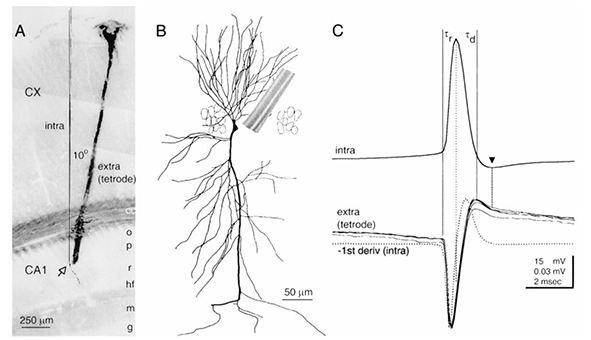
\includegraphics{Figures/Spikes/Spikes-Henze-w100-r150}
\end{center}
\caption[Intracellular and extracellular action potentials]{\textbf{Simultaneous recording of intracellular and extracellular action potentials (`spikes').}
Adapted from \citeasnoun**{Henze2000}.
\gen{Figure + caption to be updated}
}
\label{fig:Spikes:Henze}
\end{figure}
%%%%%%%%%%%

\ghnote{Avsnittet nedenfor var langt, og inneholdt veldig mye forskjellig. Jeg delte det opp. Foreslaar at vi ogsaa legger inn referanser til underkapitler hvor de ulike tema behandles.}

\gex{The amplitude of the membrane-potential deflection during an action potential is about 100~mV. The amplitude of \ghtxt{a }spike\sout{s}, a term which we in the present book restrict to the extracellular signature of action potentials,} \ghtxt{\sout{are} is} typically less than 1~mV. Also, the shape of the spike is very different from the shape of intracellularly recorded action potentials (\Fref{fig:Spikes:Henze}). \ghnote{La inn avsnitt: De to setn. over la opp til at naa skal vi sammenligne APs vs Spikes, men det som kom under handler om aa beskrive spikes. Kanskje en setning til her om sammenligning: F.eks. si at spike-shape utenfor soma er saann ca invertert jmf AP?}

The initial sharp negative peak is often referred to as the `sodium peak' as it mainly stems from sodium ions flowing into the soma (and axon hillock) during the initial phase of the action potential. The later blunter positive peak is likewise sometimes referred to as the `potassium peak', as it is dominated by potassium ions flowing out of the soma. \ghnote{Her er det vel implisitt at vaar spike er i naerheten av soma? Burde kanskje si dette eksplisitt?} 

\ghnote{Byttet avsnitt: Nytt tema: Detection:} When detecting spikes, the main issue is that the spike amplitude must be larger than the ambient noise level, typically some tens of \si{\micro\volt}. \ghnote{Har litt problemer med ansatsen: The main issue er noise - og saa snakker vi ikke mer om det...}
%\gen{Har vi et godt tall med medhoerende referanse her?} 
%\ehnote{Tja. Ambient noise er jo veldig avhengig av forskjellige faktorer, elektrode-type og impedans, in vivo vs. in vitro, vaaken vs. bedoevet tilstand osv, valg av filter, osv.}
%\tvnnote{Alessio sa de typisk ikke tar med spikes med amplitude under 30 uV, og det var dette vi brukte i Buccino et al., 2018, J Neurophysiol, men han hadde ikke noe god kilde ellers}
For the detection of spikes, the detailed spike shape is of less importance. However \ghnote{er dette et "men" til forrige paastand?}, an extracellular electrode will in general measure spikes from several neurons positioned in the vicinity of the electrode contact. To obtain spike trains from individual neurons, the recorded spikes must thus be sorted in a process referred to as spike sorting~\cite**{Quiroga2007}. In this process, the differences in spike shapes are crucial~\cite**{Einevoll2012}. Spike shapes are also used to distinguish spikes from different neuron types~\cite**{Bartho2004}. The temporal width of the spike is, for example, used to separate putative inhibitory neurons (narrow spikes) from excitatory neurons (broad spikes), but a more detailed separation into subgroups is also possible~\cite**{Buccino2018}. 

Detailed modeling of spikes are important for several reasons: for example, (i) to understand the relationship between single-neuron properties and spike shapes \cite**{Holt1999,Gold2006,Pettersen2008a,Anastassiou2013}, (ii) to estimate biases regarding which types of neurons that are most likely to generate the spikes recorded by electrodes \cite**{Pettersen2008a},
(iii) to provide benchmarking data for development and testing of methods for spike sorting or spike-based neuron identification \cite**{Einevoll2012,CamunasMesa2013,Hagen2015,MondragonGonzalez2017,Buccino2020}, and (iv) to fit model parameters in multicompartment neuron models \cite**{Gold2007}.


%%%%
\section{\blue{Recording of spikes: GH - nytt forslag}}
\label{sec:Spikes:recording}
\ghnote{Skrev et nytt forslag til dette delkapittelet basert paa kommentarer til forrige versjon.}
Spike recordings are typically done in living brains. 
As we have seen, an action potential is a rapid deflection in the neuronal membrane potential
taking place within a time window of just a few milliseconds.
As its extracellular signature, the spike, will have a similarly fast time coarse, 
it is common to study it by concentrating on the high frequencies of the extracellular potential.
Accordingly, the signal used for analyzing spiking activity is 
typically obtained by high-pass filtering the extracellular potential using a lower cut-off set at some hundred hertz. 
In contrast, the low-frequency part, the local field potential (LFP), 
is thought to mostly reflect synaptic inputs onto populations neurons around the contact~\cite**{Einevoll2013}, 
see \Fref{chap:LFP}.

The above does not imply that the spike is built up exclusively of high-frequency components.
This is a common misunderstanding, and the reasoning behind it is that, 
since a spike typically lasts only a couple of milliseconds and an oscillation with a period of, say, 
2 milliseconds corresponds to a frequency of 500 hertz, 
frequencies lower that this should be absent or at least very weak. 
However, this is not generally true for spikes ~\cite**{Pettersen2008,Schomburg2012,Ray2011,Scheffer-Teixeira2013},
and the main reason is that spikes are not single frequency oscillations.
In general, one can not deduce the frequency content of a signal merely from its briefness. 
This is perhaps best illustrated by the so-called Dirac $\delta$ function 
which essentially is infinitely sharp and has zero width, 
but is built up of equal amounts of frequency components for all frequencies (\Fref{fig:Spikes:freq_dep_delta}). 

%%%%%%%%%
% Figure
%%%%%%%%%
\begin{figure}[!ht]
\begin{center}
%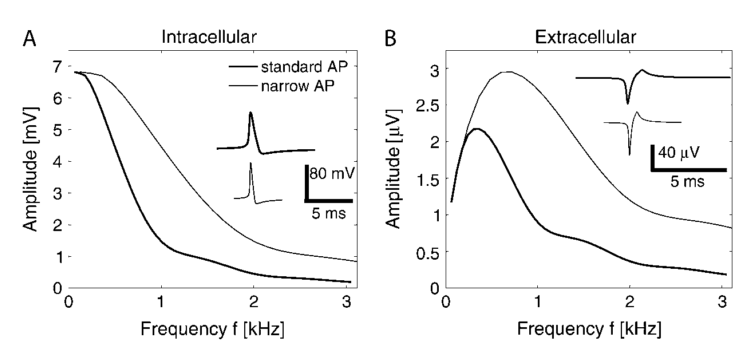
\includegraphics[width=0.6\textwidth]{Figures/Spikes/Spikes-eap_illustration.png}
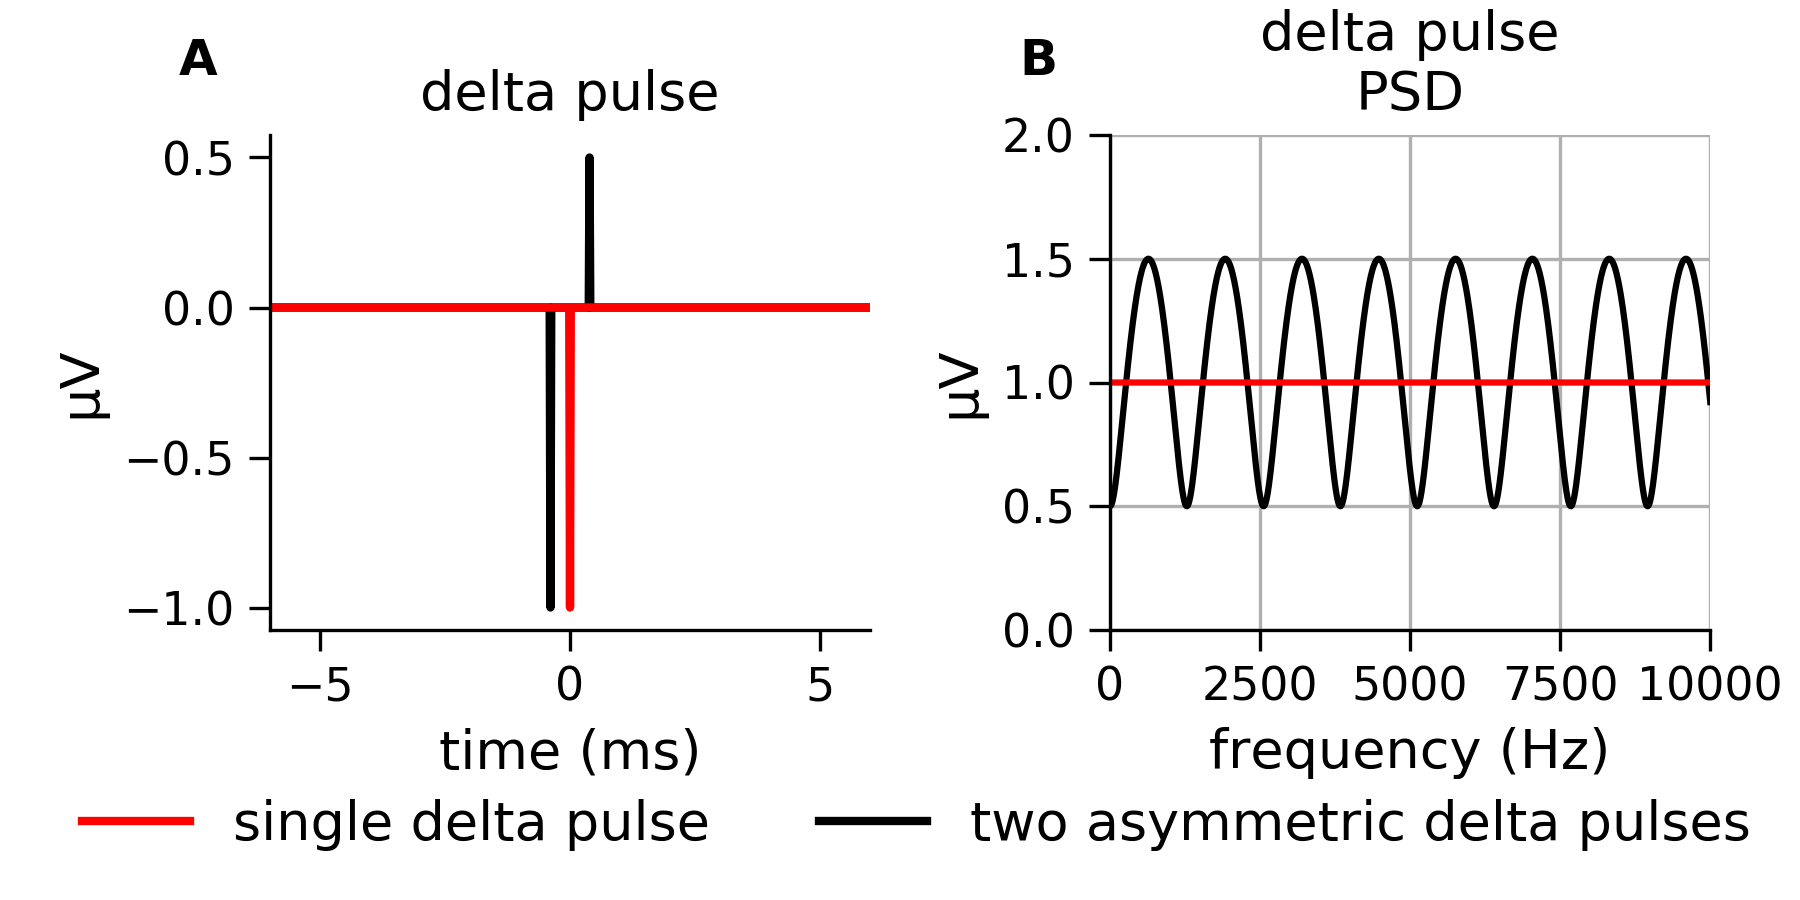
\includegraphics[width=1.0\textwidth]{Figures/Spikes/Spikes-fig_delta_pulse_freq_content.png}
\end{center}
\caption{\textbf{Delta pulses and frequency content.}
A single delta-pulse (panel A, red) has frequency components with equal contributions for all frequencies (panel B, red).
An asymmetric pair of delta-pulses, caricaturing the spike in \Fref{fig:Spikes:freq_dep}B with a negative sodium peak followed by a weaker positive potassium peak (panel A, black), instead has an oscillating frequency spectrum (panel B, black). This spectrum has its (first) maximum at 625 Hz, but also has substantial contributions from frequencies all the way down to zero.
\gen{Kanskje la x-aksen faa fra 0 till 2000 Hz som i Fig. 8.2B? Tar vel ogsaa bort bakgrunns-rutegrid i B? Enhet paa y-akse i B maa fikses. Kanskje vi kan velge -100 $mu$V som amplitude paa sodium-pulse i A slik at det ligner mer paa  Fig. 8.2?}
}
\label{fig:Spikes:freq_dep_delta}
\end{figure}
%%%

Even a fast sodium spike contains frequency components with frequencies as low as 100 Hz \cite**{Pettersen2008a}. 
This is illustrated in \Fref{fig:Spikes:freq_dep} showing that also very narrow spikes may contain low-frequency components. 
In addition, the sodium spike may coincide with slower spike-associated phenomena such as calcium spikes~\cite**{Stuart2007} and spike afterhyperpolarization \cite**{Buzsaki1988} which may further contribute to increased low-frequency components~\cite**{Buzsaki2012}.
\gex{\citeasnoun**{anastassiou2015b} found, for example, spike contributions to the LFPs for frequencies as low as 20 Hz for cortical pyramidal neurons, likely stemming from such spike afterhyperpolarization.}

%%%%%%%%%
% Figure
%%%%%%%%%
\begin{figure}[!ht]
\begin{center}
%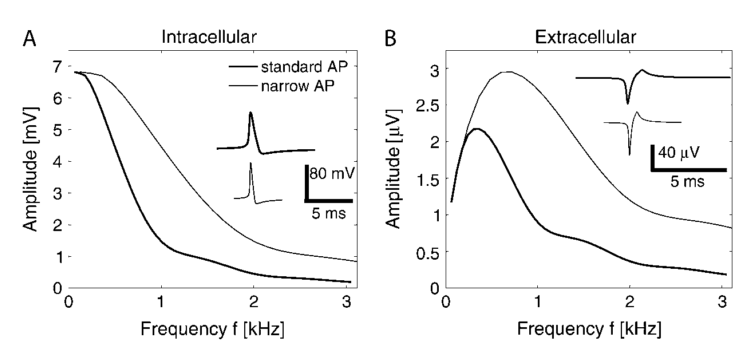
\includegraphics[width=0.6\textwidth]{Figures/Spikes/Spikes-eap_illustration.png}
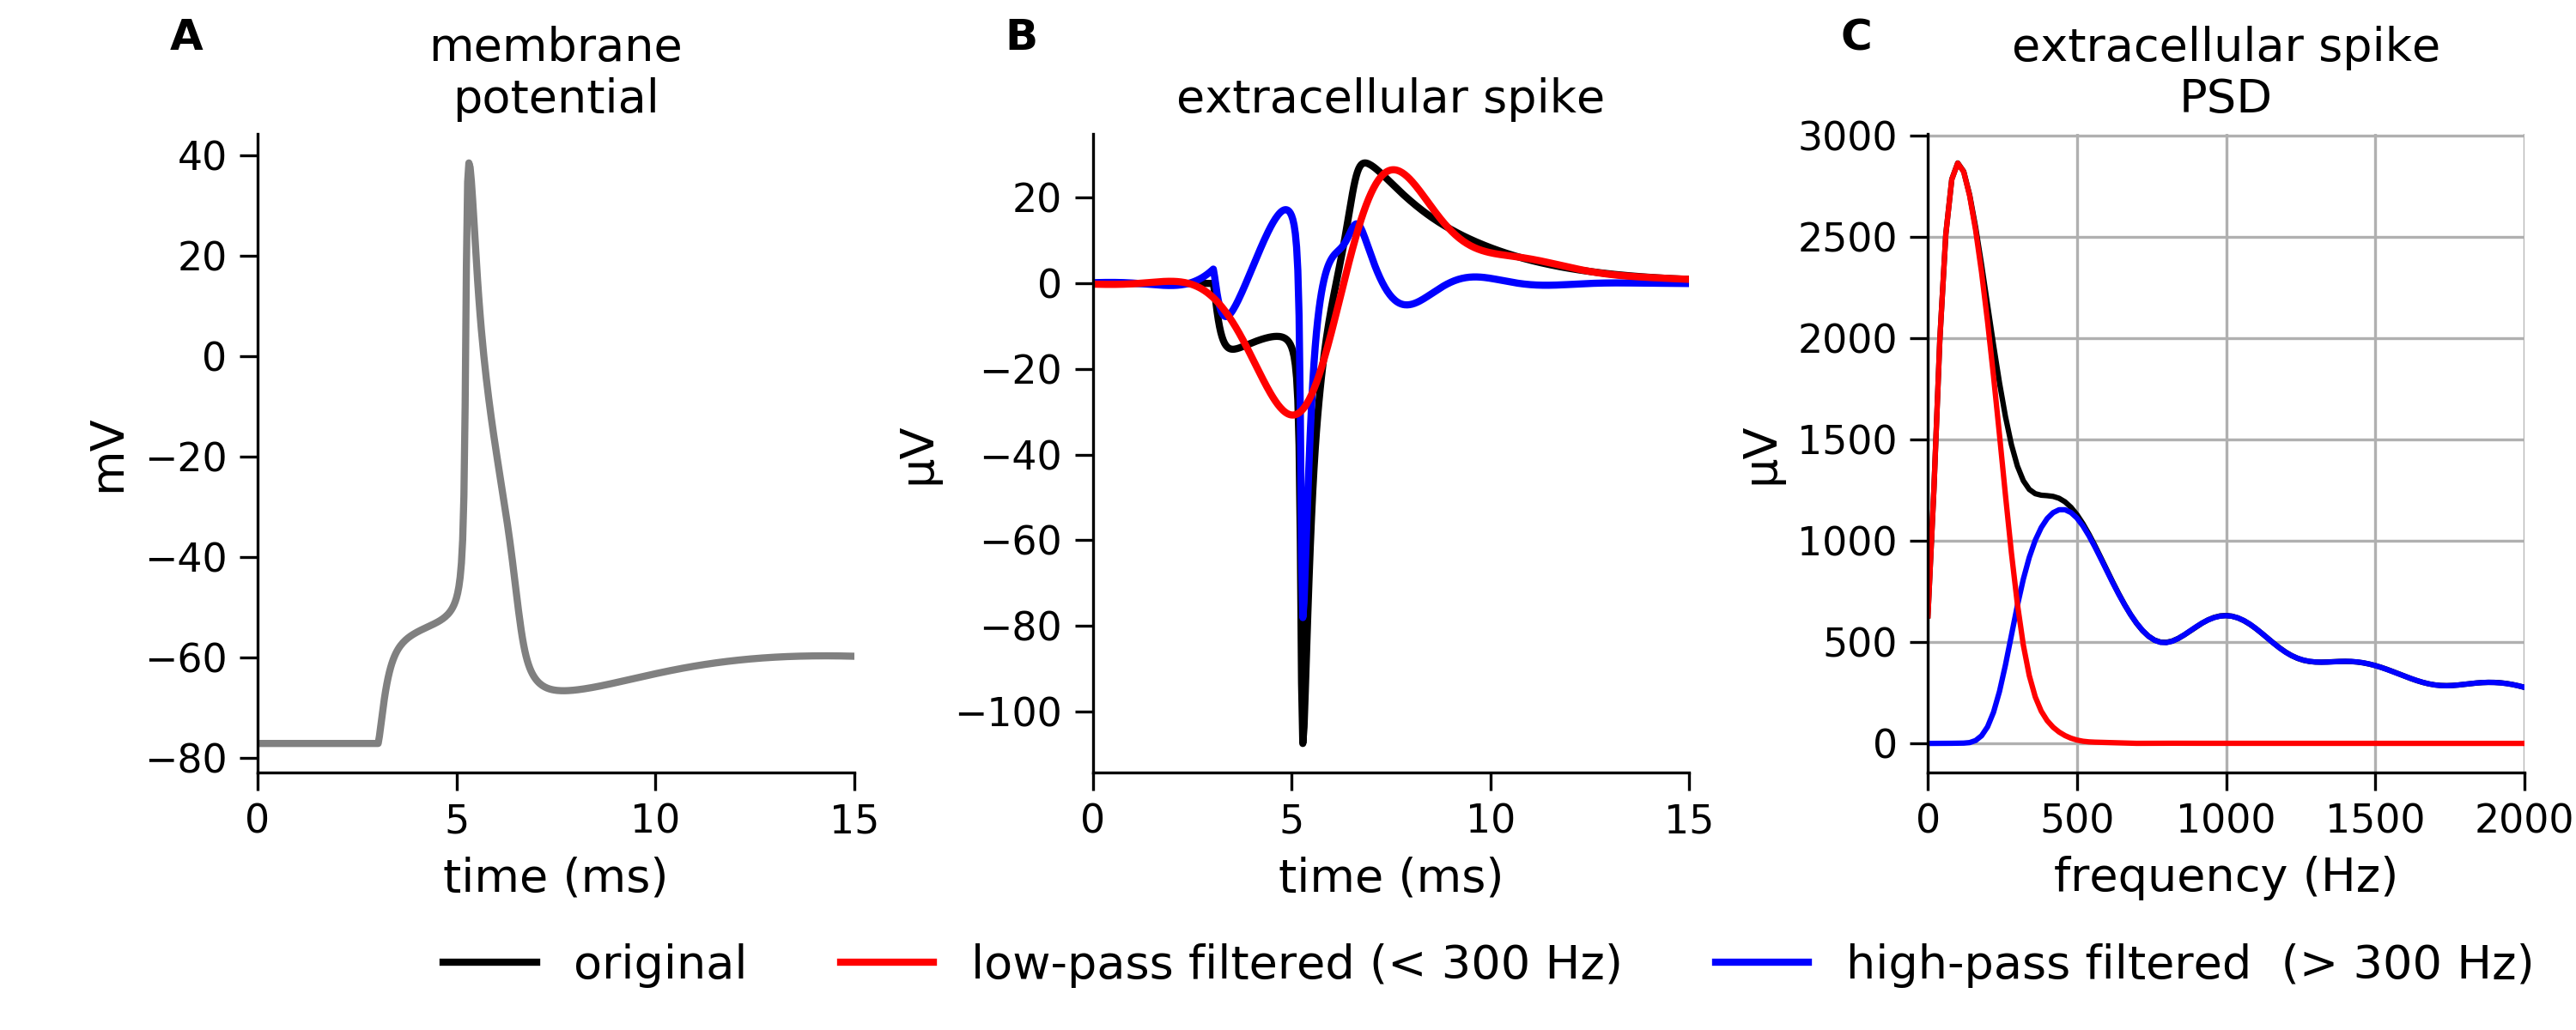
\includegraphics[width=1.0\textwidth]{Figures/Spikes/Spikes-fig_spike_freq_content_amp.png}
\end{center}
\caption[]{\textbf{Spike and frequency components.}
A: Membrane potential during firing of action potential of Hay neuron \cite**{Hay2011}. \ghnote{For aa sitere i figurtest, legg inn en klamme rett etter caption[].}
B: Corresponding extracellular spike measured \gex{XX $\mu$m} outside of soma neurons. Raw signal (black),
low-pass filtered signal (red), high-pass filtered signal (blue).
C: Frequency content of signals in B, that is, amplitudes for frequency components found by Fourier transformation.
\gen{Kanskje vi kunne legge til Fourier spektrum for intracellular action potentials ogsaa slik at vi kan kommentere
at ikke bare spike-formen i tid, men ogsaa i frekvens, er veldig forskjellig?}
\gen{Enhet paa y-akse i C maa fikses. Tar vel ogsaa bort bakgrunns-rutegrid i C?}
\ehnote{hvordan er den cella stimulert? Ser ut som en stroempuls som vil gi et stort bidrag i PSD. Jeg foreslaar DC input som gir persistent fyring med lav rate, saa kan du heller regne ut PSD fra en enkelt spike.}  
}
\label{fig:Spikes:freq_dep}
\end{figure}
%%%%%

The motivation for performing a high-pass filtering of extracellular potential when detecting spikes
is not that spikes do not contain frequency components below the cut-off, 
but rather that one in that way may hope to isolate the spike signal from other slower neural processes. 
While these other slower processes typically dominate the extracellular potential in terms of overall signal power, 
they have very little power above a few hundred hertz and can thus be removed with high-pass filtering ~\cite**{Pettersen2008,Einevoll2013}.

Overviews over the challenges when measuring spikes can be found in  \citeasnoun**{Anastassiou2013} and \citeasnoun**{Whittingstall2013}. \gen{Noen andre mulige referanser her?} 


 


%%%
\section{\blue{Recording of spikes}}
\label{sec:Spikes:recording}
Spike recordings are typically done in living brains, and the signal is obtained by high-pass filtering the extracellular potentials, with a lower cut-off set at some hundred hertz. In contrast, the low-frequency part, the local field potential (LFP), is thought to mostly reflect synaptic inputs onto populations neurons around the contact~\cite**{Einevoll2013},
see \Fref{chap:LFP}.

\snnote{Jeg lurte paa om det kanskje hadde vaert fint aa starte enda mer basic? Hva med aa forst forklare hva spikes har med high-pass filtering aa gjore, og videre motivere high-pass filtering ved aa flytte det nest siste avsnittet i denne seksjonen opp hit? Har et forslag, men det er kanskje litt too much:}

\sntxt{Since action potentials travel fast \ghnote{"travel" faar meg til aa tenke propagering opp akson, men det er vel ikke det som er poenget?)}, the resulting spikes picked up by electrodes in brain tissue represent rapid changes in the electric potential. The suddenness of spikes implies that these signals contain high frequencies. When studying spiking activity, we can concentrate on the high frequencies by \textit{high-pass filtering} the electric potentials. The lower cutoff is typically set at a few hundred hertz.}

\snnote{Og saa legge til avsnittet "The high-pass filtering of the extracellular potential..."?}

A common misunderstanding is that a spike is built up only of high-frequency components. The reasoning is that, since a spike typically lasts only a couple of milliseconds and an oscillation with a period of, say, 2 milliseconds corresponds to a frequency of 500 hertz, lower frequencies will be absent or at least very weak. However, this is not generally true~\cite**{Pettersen2008,Schomburg2012,Ray2011,Scheffer-Teixeira2013}. Even a fast sodium spike contains frequency components with frequencies as low as 100 Hz \cite**{Pettersen2008a}. 
\ehnote{Edit: Artikkelen jeg hadde i tankene var Anastassiou et al 2015: 10.1152/jn.00628.2014. Abstract: "... We found that spiking of excitatory neurons can significantly impact the LFP at frequencies as low as 20 Hz. Our results question the common assertion that the LFP acts as proxy for synaptic activity."} 
\gen{Nyttig tips: Men slik jeg leser artikkelen saa er tolkningen at dette skyldes spike "afterhypolarization". Har lagt inn en setning om det lenger ned.} 
This is illustrated in \Fref{fig:Spikes:freq_dep} showing that also very narrow spikes may contain low-frequency components. In fact, the so-called Dirac $\delta$ function which essentially is infinitely sharp and has zero width, is built up of equal amounts of frequency components for all frequencies. In addition, the sodium spike may coincide with slower spike-associated phenomena such as calcium spikes~\cite**{Stuart2007} and spike afterhyperpolarization \cite**{Buzsaki1988} which may further contribute to increased low-frequency components~\cite**{Buzsaki2012}.
\gex{\citeasnoun**{anastassiou2015b} found, for example, spike contributions to the LFPs for frequencies as low as 20 Hz for cortical pyramidal neurons, likely stemming from such spike afterhyperpolarization.}



%%%%%%%%%
% Figure
%%%%%%%%%
%\begin{figure}[!ht]
%\begin{center}
%%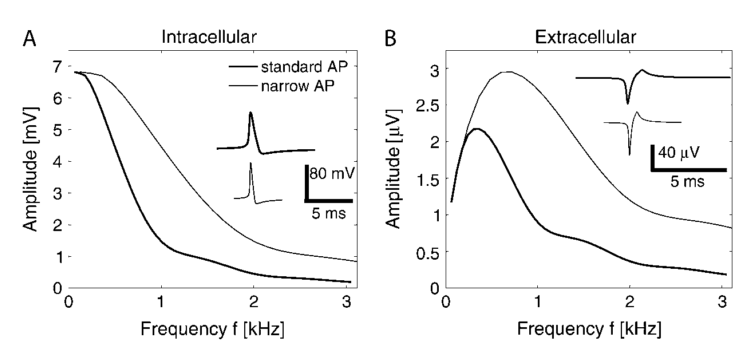
\includegraphics[width=0.6\textwidth]{Figures/Spikes/Spikes-eap_illustration.png}
%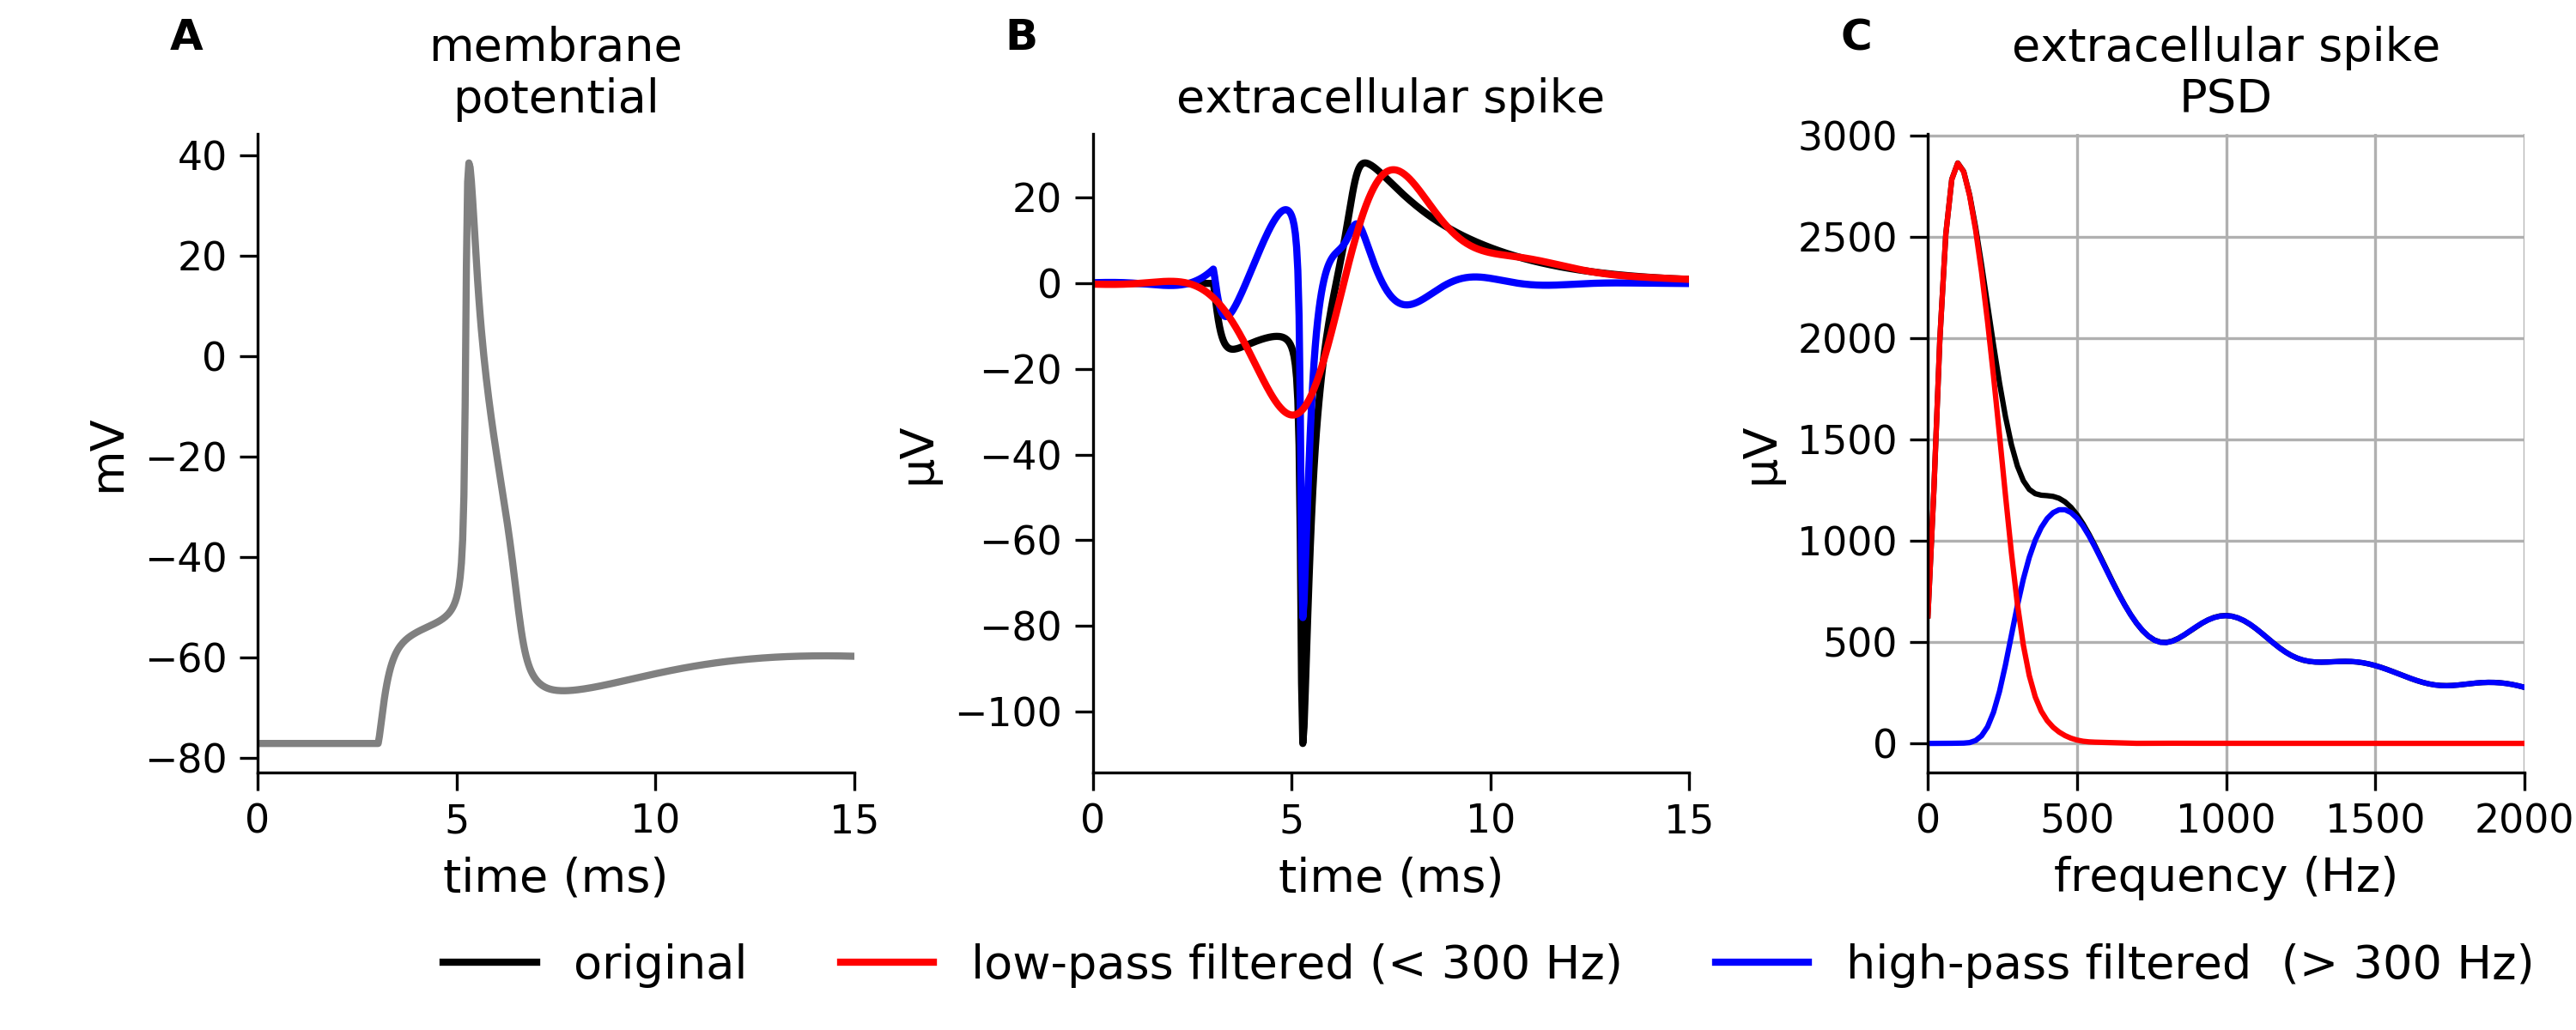
\includegraphics[width=1.0\textwidth]{Figures/Spikes/Spikes-fig_spike_freq_content_amp.png}
%\end{center}
%\caption[]{\textbf{Spike and frequency components.}
%A: Membrane potential during firing of action potential of Hay neuron \cite**{Hay2011}. \ghnote{For aa sitere i figurtest, legg inn en klamme rett etter caption[].}
%B: Corresponding extracellular spike measured \gex{XX $\mu$m} outside of soma neurons. Raw signal (black),
%low-pass filtered signal (red), high-pass filtered signal (blue).
%C: Frequency content of signals in B, that is, amplitudes for frequency components found by Fourier transformation.
%\gen{Kanskje vi kunne legge til Fourier spektrum for intracellular action potentials ogsaa slik at vi kan kommentere
%at ikke bare spike-formen i tid, men ogsaa i frekvens, er veldig forskjellig?}
%\gen{Enhet paa y-akse i C maa fikses. Tar vel ogsaa bort bakgrunns-rutegrid i C?}
%\ehnote{hvordan er den cella stimulert? Ser ut som en stroempuls som vil gi et stort bidrag i PSD. Jeg foreslaar DC input som gir persistent fyring med lav rate, saa kan du heller regne ut PSD fra en enkelt spike.}  
%}
%\label{fig:Spikes:freq_dep}
%\end{figure}
%%%%%

%%%%%%%%%
% Figure
%%%%%%%%%
%\begin{figure}[!ht]
%\begin{center}
%%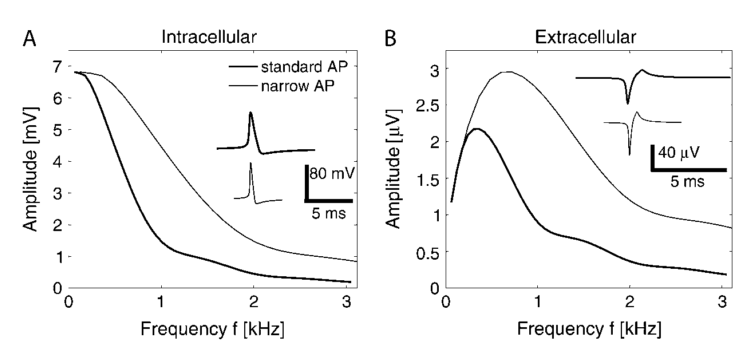
\includegraphics[width=0.6\textwidth]{Figures/Spikes/Spikes-eap_illustration.png}
%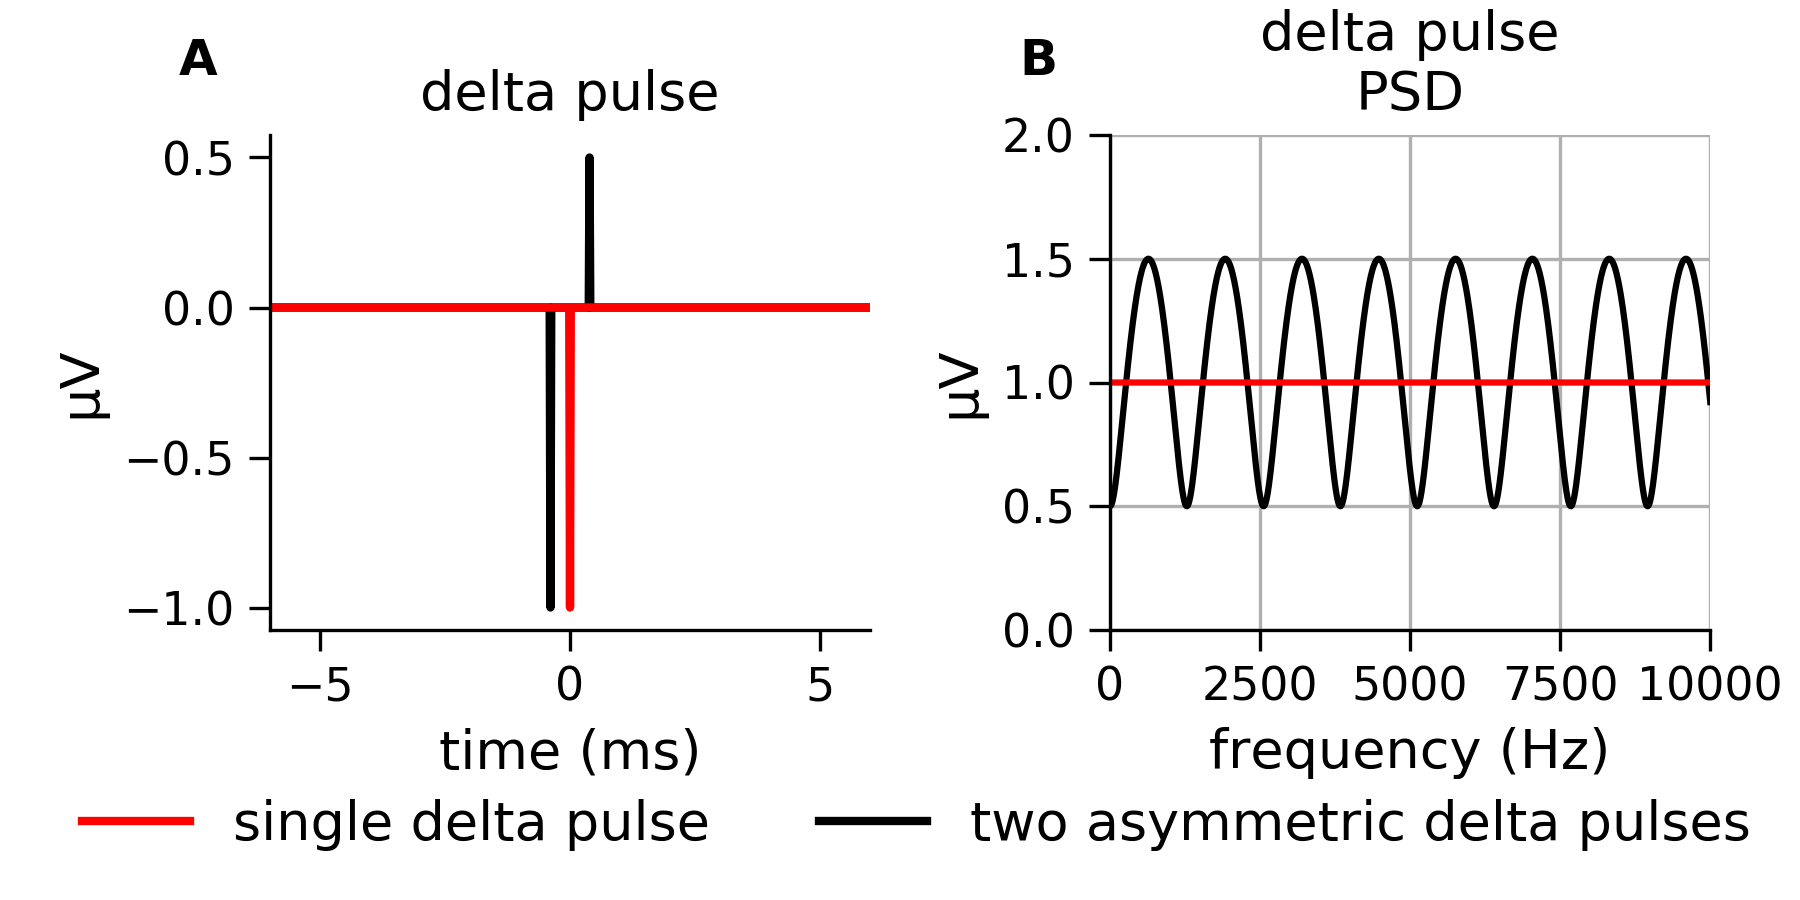
\includegraphics[width=1.0\textwidth]{Figures/Spikes/Spikes-fig_delta_pulse_freq_content.png}
%\end{center}
%\caption{\textbf{Delta pulses and frequency content.}
%A single delta-pulse (panel A, red) has frequency components with equal contributions for all frequencies (panel B, red).
%An asymmetric pair of delta-pulses, caricaturing the spike in \Fref{fig:Spikes:freq_dep}B with a negative sodium peak followed by a weaker positive potassium peak (panel A, black), instead has an oscillating frequency spectrum (panel B, black). This spectrum has its (first) maximum at 625 Hz, but also has substantial contributions from frequencies all the way down to zero.
%\gen{Kanskje la x-aksen faa fra 0 till 2000 Hz som i Fig. 8.2B? Tar vel ogsaa bort bakgrunns-rutegrid i B? Enhet paa y-akse i B maa fikses. Kanskje vi kan velge -100 $mu$V som amplitude paa sodium-pulse i A slik at det ligner mer paa  Fig. 8.2?}
%}
%\label{fig:Spikes:freq_dep_delta}
%\end{figure}
%%%%

\gex{The high-pass filtering of the extracellular signal typically used when detecting spikes in extracellular recordings, is done to isolate the spike signal from other slower neural processes. While the signals from these other slower processes typically
dominate in terms of overall signal power, they have very little power above a few hundred hertz and can thus be removed with high-pass filtering ~\cite**{Pettersen2008,Einevoll2013}.} 
%\ghnote{Er ikke dette en tautologi? The low-frequency part has little power in the high frequencies?}

Overviews over the challenges when measuring spikes can be found in  \citeasnoun**{Anastassiou2013} and \citeasnoun**{Whittingstall2013}.
\gen{Noen andre mulige referanser her?} 

 %%%%%%%%%%
% Figure: Spike from multi-compartment model
%%%%%%%%%%
%\begin{cnfigure}{Figures/mm/EP-spike-MultiCompartment-w100-r150}
%\begin{figure}[!ht]
%\begin{center}
%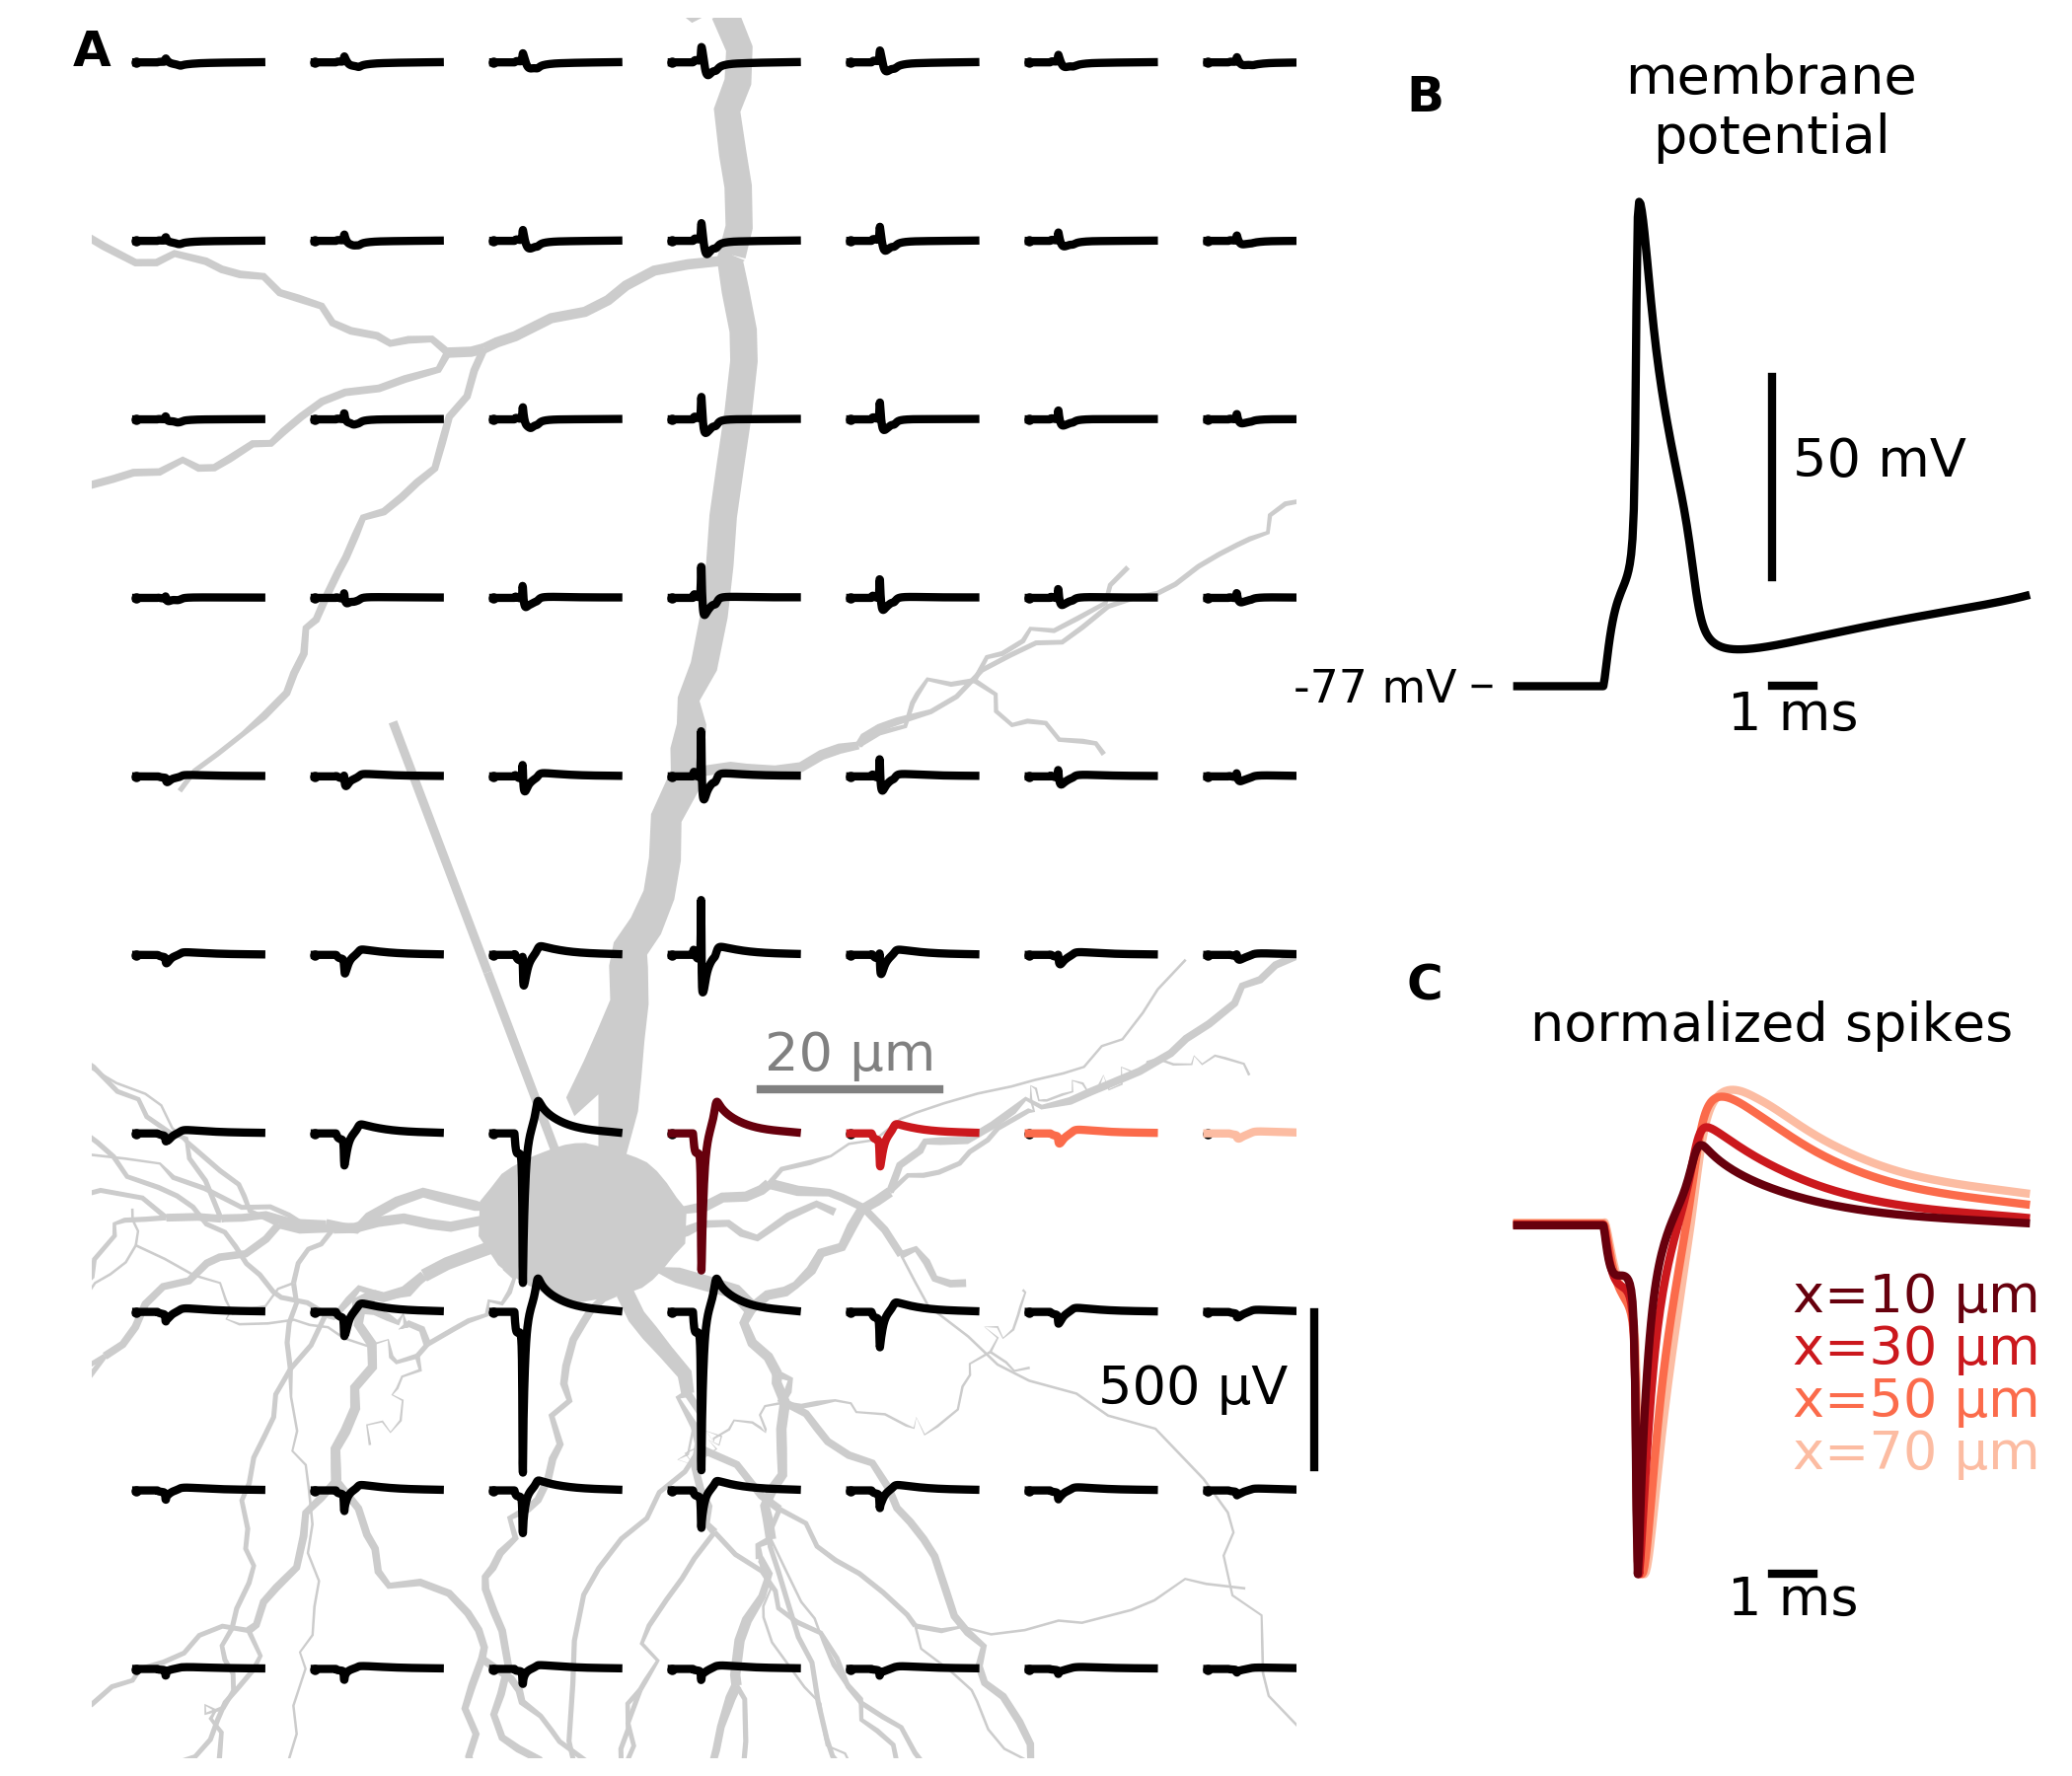
\includegraphics[width=1.0\textwidth]{Figures/Spikes/Spikes-fig_hay_eap_simpler}
%\end{center}
%\caption[]{\textbf{Spike from action potential for a multi-compartmental neuron model.}
%A: Spikes computed at different positions around example Hay-neuron \cite**{Hay2011} using \gex{Eq. XX}.
%B: Corresponding membrane potential. C: Spike shapes at different lateral positions in A as depicted by colouring. Spike shapes
%are normalized to have the same magnitude of the negative peak.
%The action potential was generated by injection of synaptic currents into the soma of the model neuron. 
%\ehnote{Figure adapted from Fig4. i Hagen2015 kanskje? Aksonet peker i "feil" retning ogsaa. 
%Det boer nevnes hva som driver depolariseringen, ser ut som en step current?}
%\tvnnote{Vi ville ha en litt enklere versjon enn Fig. 4 i Hagen2015, men enig i at vi kanskje boer vurdere aa fikse retningen til axonet. Har du koden for dette? Stimuli er foreloebig synaptisk input i soma} \ghnote{Denne figuren er panel A i neste figur. Foreslaar at den fjernes, og at vi refererer dit.} 
%\gen{Synes det er fint aa ha den her i stort format siden den paa en maate er "ground truth" i denne sammenheng.}
%}. 
%Active sodium
%and potassium conductances in the soma compartment and computed from 
%\Fref{XX:equation:Ve-multi-compartment}.
%Left panel shows the EP at different spatial positions, while right panel shows the corresponding
%soma membrane potential during the action potential. 
%\gen{Figure + caption to be updated. Change to Hay-model,}
%\label{fig:Spikes:MultiCompartment}
%%\figpermOurs
%\end{figure}

%%%

\section{\blue{Modeling spikes}}
\label{sec:Spikes:modeling spikes}
\subsection{\blue{Spikes from multi-compartment neuron models}}
\label{sec:Spikes:multi-compartment}
%%%
%\ghnote{Forslag: Sec 8.2, 8.3, 8.4.1 slaas sammen til delkapitler i 8.2. som heter modeling spikes eller noe. Formaal er aa vise eksempelsimuleringer for ulike morfologier. Analysen kommer senere i nytt 8.3. og er der for enkelhets skyld i stor grad basert paa ball-and-stick. 8.3. kan gjoeres litt mer up-front med tanke paa introdusering av Fourier-greier, og vi kan referere dit i 8.1 der vi viser Fourier-resultater uten aa ha introdusert teorien. Evt. kan vi introudsere Fourier tidligere et sted, feks. i VC-kapittelet eller som eget kapittel?}
The somatic intracellular action potential in a given neuron has a quite stereotypical waveform, 
i.e., all action potentials fired by the same neuron have more or less the same shape. 
The shape and amplitude of the extracellular spike that it generates will, however, 
depend strongly on the position where it is recorded. 
This is illustrated in \Fref{fig:Spikes:MultiCompartment} showing computed spikes at various positions around a neuron during the firing of an action potential. 
Here the scheme described in \Fref{sec:Schemes:LFPy} is used with a biophysically detailed neuron model for a layer-5 pyramidal cell. 
\ghnote{Mange schemes ble vel beskrevet i det kapittelet. Kanskje putte denne info inn i figurtekst og vaere mer presis?}
One striking feature is the rapid decay of spike amplitude with distance from the soma. 
Another is the changing shape of the spike highlighted in panel C: 
The sharpest spikes are seen for recording close to the soma. 
This blunting, or low-pass filtering, of the spike with distance stems from the cable properties of the neuron, 
and has been referred to as `intrinsic dendritic filtering' \cite**{Linden2010,Pettersen2012} 
(as opposed to, say, possible filtering by the extracellular medium itself~\cite**{Bedard2012}). 
The origin of this intrinsic dendritic filtering effect is described below in \Fref{sec:Spikes:ball-and-stick}.

%%%%%%%%%%
% Figure: Spike from multi-compartment model
%%%%%%%%%%
%\begin{cnfigure}{Figures/mm/EP-spike-MultiCompartment-w100-r150}
\begin{figure}[!ht]
\begin{center}
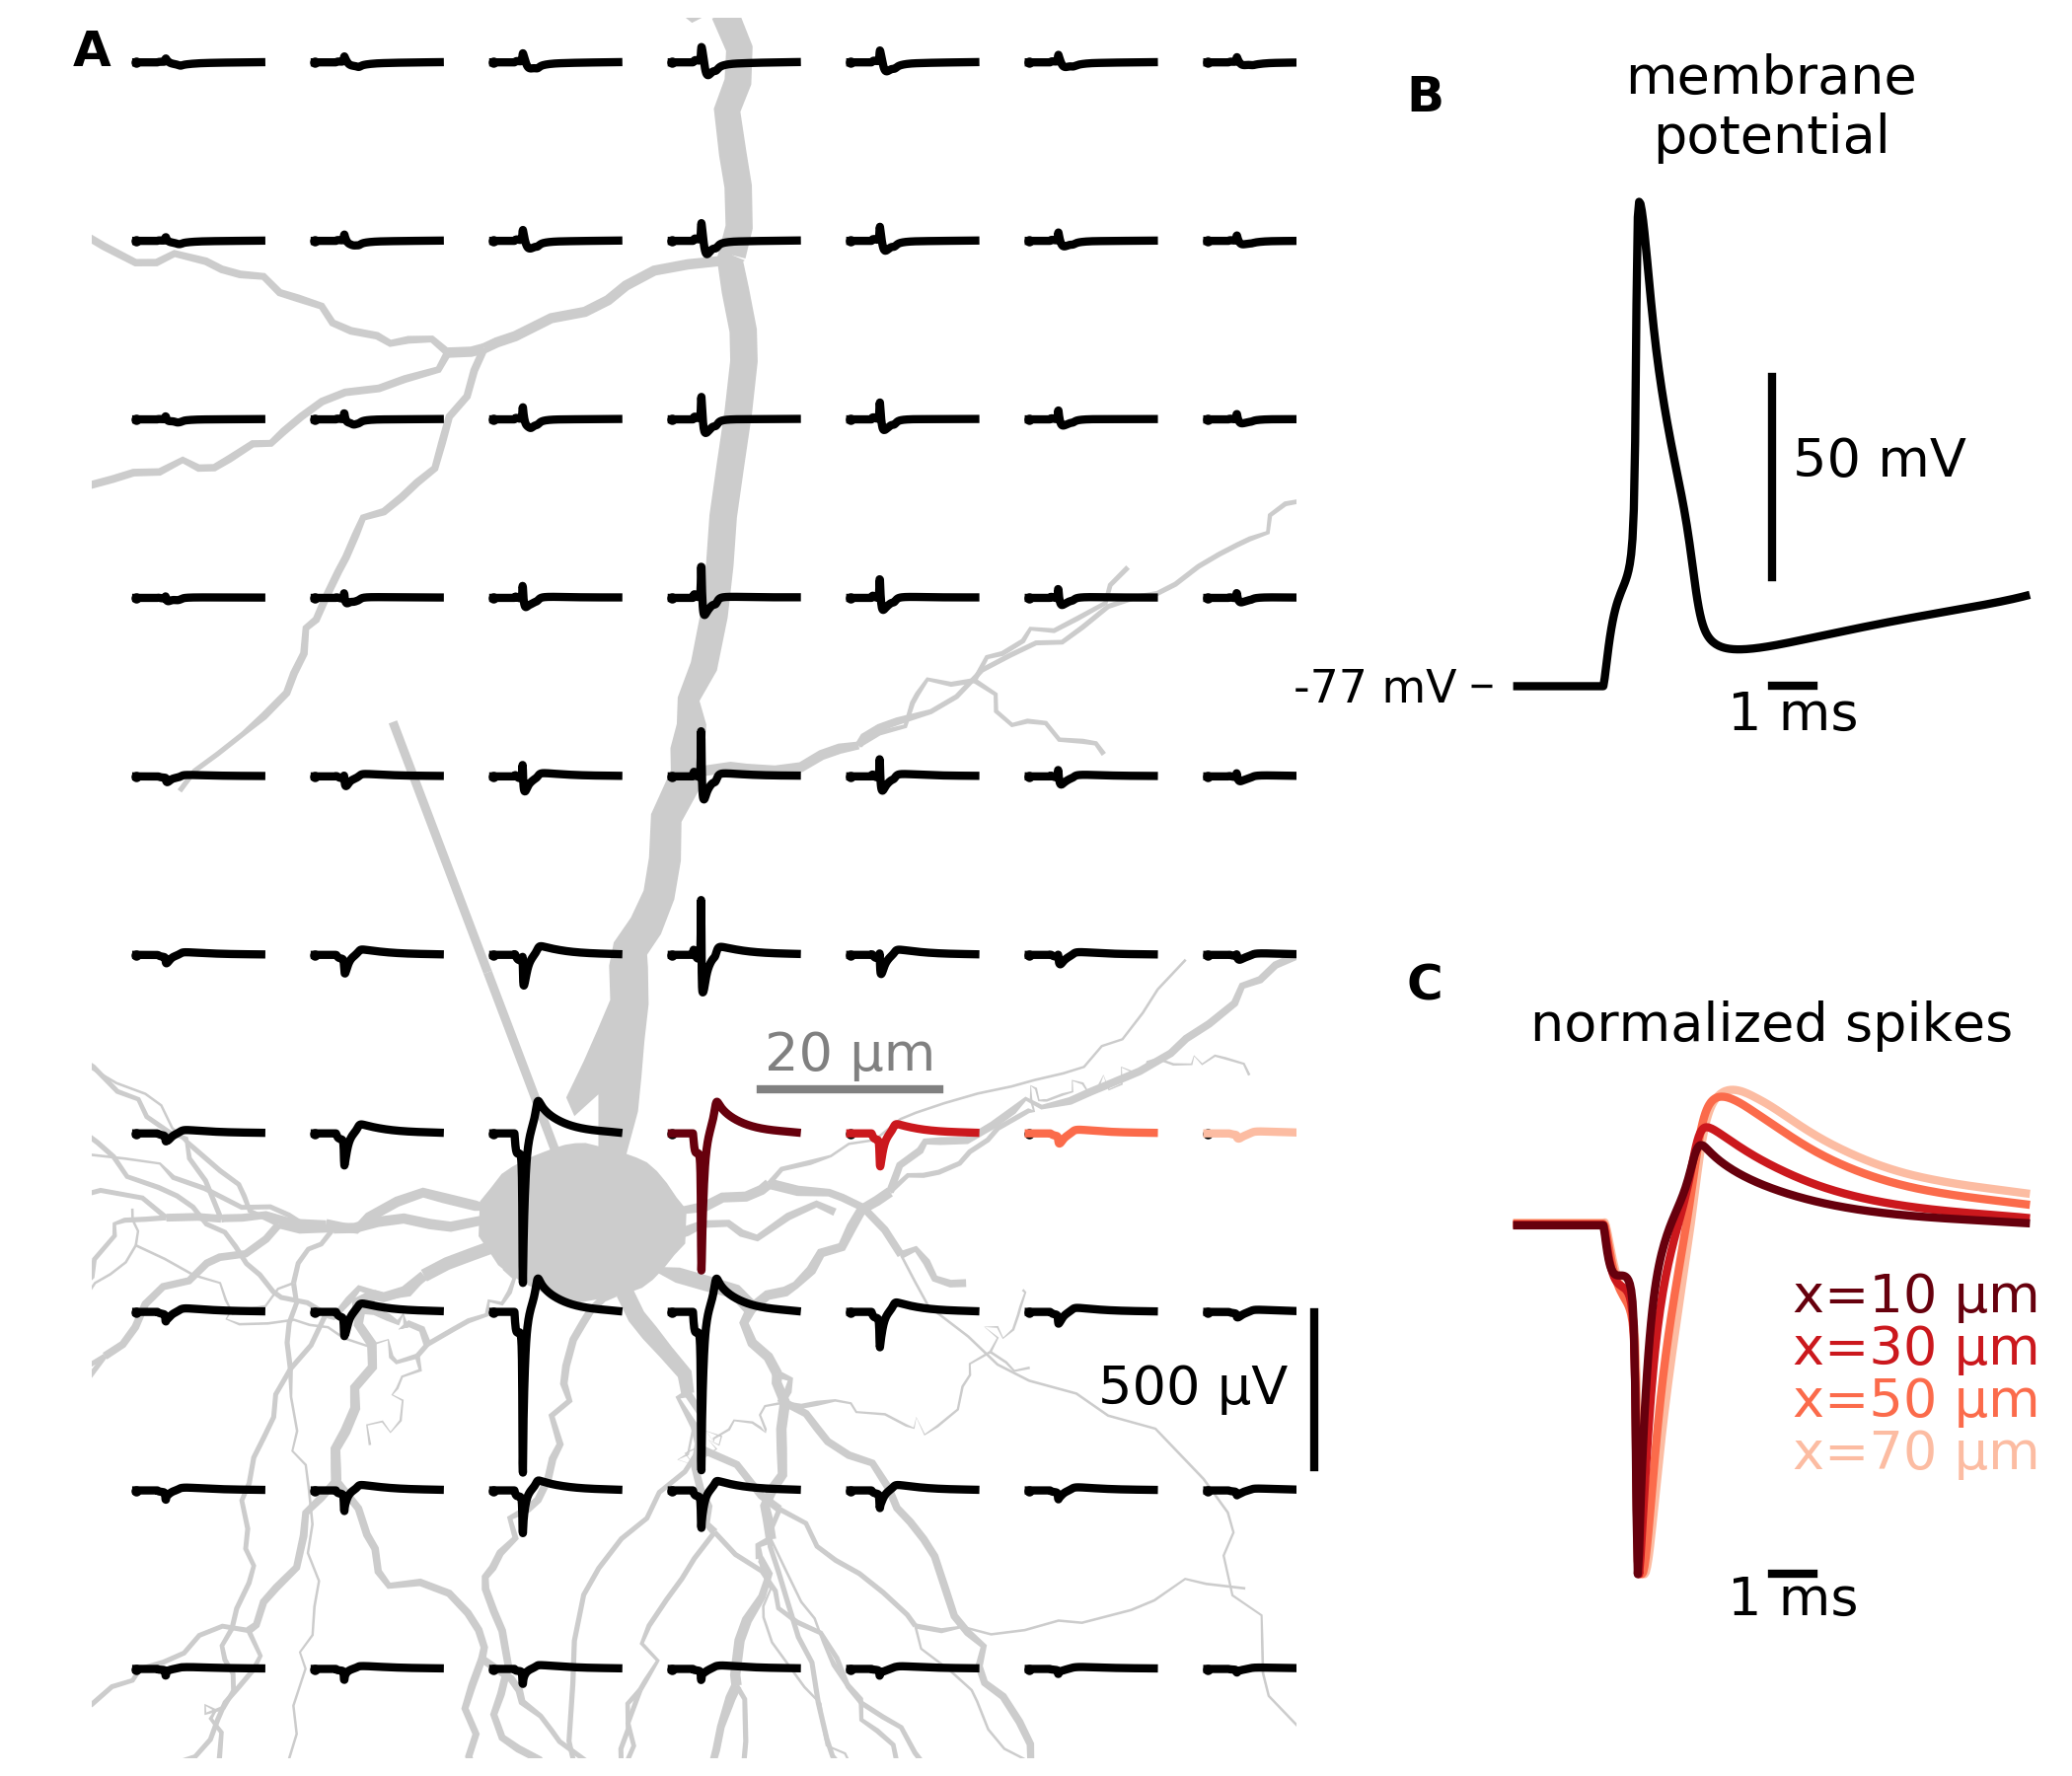
\includegraphics[width=1.0\textwidth]{Figures/Spikes/Spikes-fig_hay_eap_simpler}
\end{center}
\caption[]{\textbf{Spike from action potential for a multi-compartmental neuron model.}
A: Spikes computed at different positions around example Hay-neuron \cite**{Hay2011} using \gex{Eq. XX}.
B: Corresponding membrane potential. C: Spike shapes at different lateral positions in A as depicted by colouring. Spike shapes
are normalized to have the same magnitude of the negative peak.
The action potential was generated by injection of synaptic currents into the soma of the model neuron. 
\ehnote{Figure adapted from Fig4. i Hagen2015 kanskje? Aksonet peker i "feil" retning ogsaa. 
Det boer nevnes hva som driver depolariseringen, ser ut som en step current?}
\tvnnote{Vi ville ha en litt enklere versjon enn Fig. 4 i Hagen2015, men enig i at vi kanskje boer vurdere aa fikse retningen til axonet. Har du koden for dette? Stimuli er foreloebig synaptisk input i soma} \ghnote{Denne figuren er panel A i neste figur. Foreslaar at den fjernes, og at vi refererer dit.} 
\gen{Synes det er fint aa ha den her i stort format siden den paa en maate er "ground truth" i denne sammenheng.}
}. 
%Active sodium
%and potassium conductances in the soma compartment and computed from 
%\Fref{XX:equation:Ve-multi-compartment}.
%Left panel shows the EP at different spatial positions, while right panel shows the corresponding
%soma membrane potential during the action potential. 
%\gen{Figure + caption to be updated. Change to Hay-model,}
\label{fig:Spikes:MultiCompartment}
%\figpermOurs
\end{figure}



%A more detailed picture of spike shapes is obtained by considering a detailed multi-compartmental neuron model
%with a comprehensive branching structure typical for real neurons as in \Fref{fig:Spikes:MultiCompartment}.
%With this dendritic morphology the membrane currents through the dendrites are spread over a larger membrane area.
%As a result, \Fref{XX:equation:Ve-multi-compartment} predicts that the largest EP spikes will be seen
%around the soma for the example pyramidal neuron in \Fref{fig:Spikes:MultiCompartment}.  
%Around the apical dendrites, the spikes will still have an inverted shape compared to spikes close to the soma. 
%However, their amplitudes will be small, only a few microvolts, so they will not be seen in most experiments.
%
%As for the two-compartment spike model, the spike amplitude in \Fref{fig:Spikes:MultiCompartment} 
%decays sharply with distance from the neuron. In addition, the spike width increases
%with distance as demonstrated by the insets at two example positions. For the large spike recorded next to
%the soma the half-width of the spike is $\sim$0.6~ms, while at the position outside the dendrite, the half-width is increased to
%$\sim$0.7~ms. This corresponds to a low-pass filtering in the sense that the distant EP has lost some 
%high-frequency components compared to the EP close to the soma. This filtering effect is absent for the spike generated by the 
%two-compartment neuron model, and reflects that the cable properties of dendrites are important in determining 
%also the shape of recorded spikes.   
%
%*******



%%%
\subsection{\blue{Spikes from two-compartment neuron model}}
\label{sec:Spikes:two-compartment}
%%%
To what extent can the qualitative features regarding the position dependence of spikes seen 
in \Fref{fig:Spikes:MultiCompartment} be explained by simpler neuron models? 
While intracellular action potentials can be modelled with a single-compartment neuron model, 
the two-compartment model (\fref{sec:Neuron:2comp}) 
is the simplest neuron model that can provide an extracellular spike at all. 
An example of a spike generated by such a model is shown in \Fref{fig:Spikes:DifferentNeuronModels}D. 
Around the soma, characteristic spikes with a sharp negative peak followed by a slower positive hump are seen, 
in accordance with typical experimental spike recordings as exemplified in \Fref{fig:Spikes:Henze}. 
The same spikes with inverted form are observed outside the dendrite compartment. 
\ghtxt{As such inverted spikes are rarely, if ever, seen in experiments, 
this suggests that while the two-compartment model can account for large spikes recorded next to the soma, 
it is inadequate for predictions of the detailed spatial pattern of spike shapes 
that would be recorded by an electrode at different positions around a neuron. 
\sout{Such inverted spikes are rarely, if ever, seen in experiments, however. This suggests that while the two-compartment model can account for large spikes recorded next to the soma, it is inadequate for 
predictions of  the detailed spatial pattern of spike shapes that would be recorded by an electrode at different positions around a neuron.}}

Spike amplitudes in the two-compartment model are seen to decay with distance as in the multi-compartment model. 
However, the two-compartment predictions differ in that the shape of the spikes that they generate (panel D, bottom) 
does not depend on position (except for the complete inversion when crossing the lateral symmetry plane of the neuron). 
This can be readily understood from the two-compartment cable equation \ghtxt{(\fref{sec:Neuron:2comp}).} \ghtxt{\sout{circuit, \gex{see XX}.}} \ghnote{Vi har illustrert dette i tidligere figur, men ikke som kretsdiagram. La inn ref. til ligningene for kretsen.}
\ghtxt{Due to the symmetry axis in the two-compartment model (\fref{fig:Neuron:point_vs_multi}B),} \ghtxt{\sout{T}t}he transmembrane current (including the capacitive current) that enters the soma compartment must at all times equal the transmembrane current leaving the dendrite compartment. The spike will thus be set up by the sum of two monopolar contributions with the same magnitude and opposite signs, and the only feature that will vary with spike position is the net amplitude of the spike. The shape of the spike will thus always be the same \gex{when the extracellular conductivity is assumed constant as here}. \ghnote{Gjelder dette om vi beveger oss vertikalt? Er det aapenbart? Gjelder det 100 prosent? Ratio mellom distanse til kilde og distanse til sluk endrer seg jo hvis vi ikke er paa 0-aksen. Men kanskje betyr ikke det noe, ettersom kilde og sluk har identiske tidsforloep (bortsett fra at de er inverterte)? }

%%%%%%%%%%
% Figure: Spikes from two-compartment, ball-and-stick and multicompartment
%%%%%%%%%%
%\begin{cnfigure}{Figures/mm/EP-spike-TwoCompartment-w100-r150}
\begin{figure}[!ht]
\begin{center}
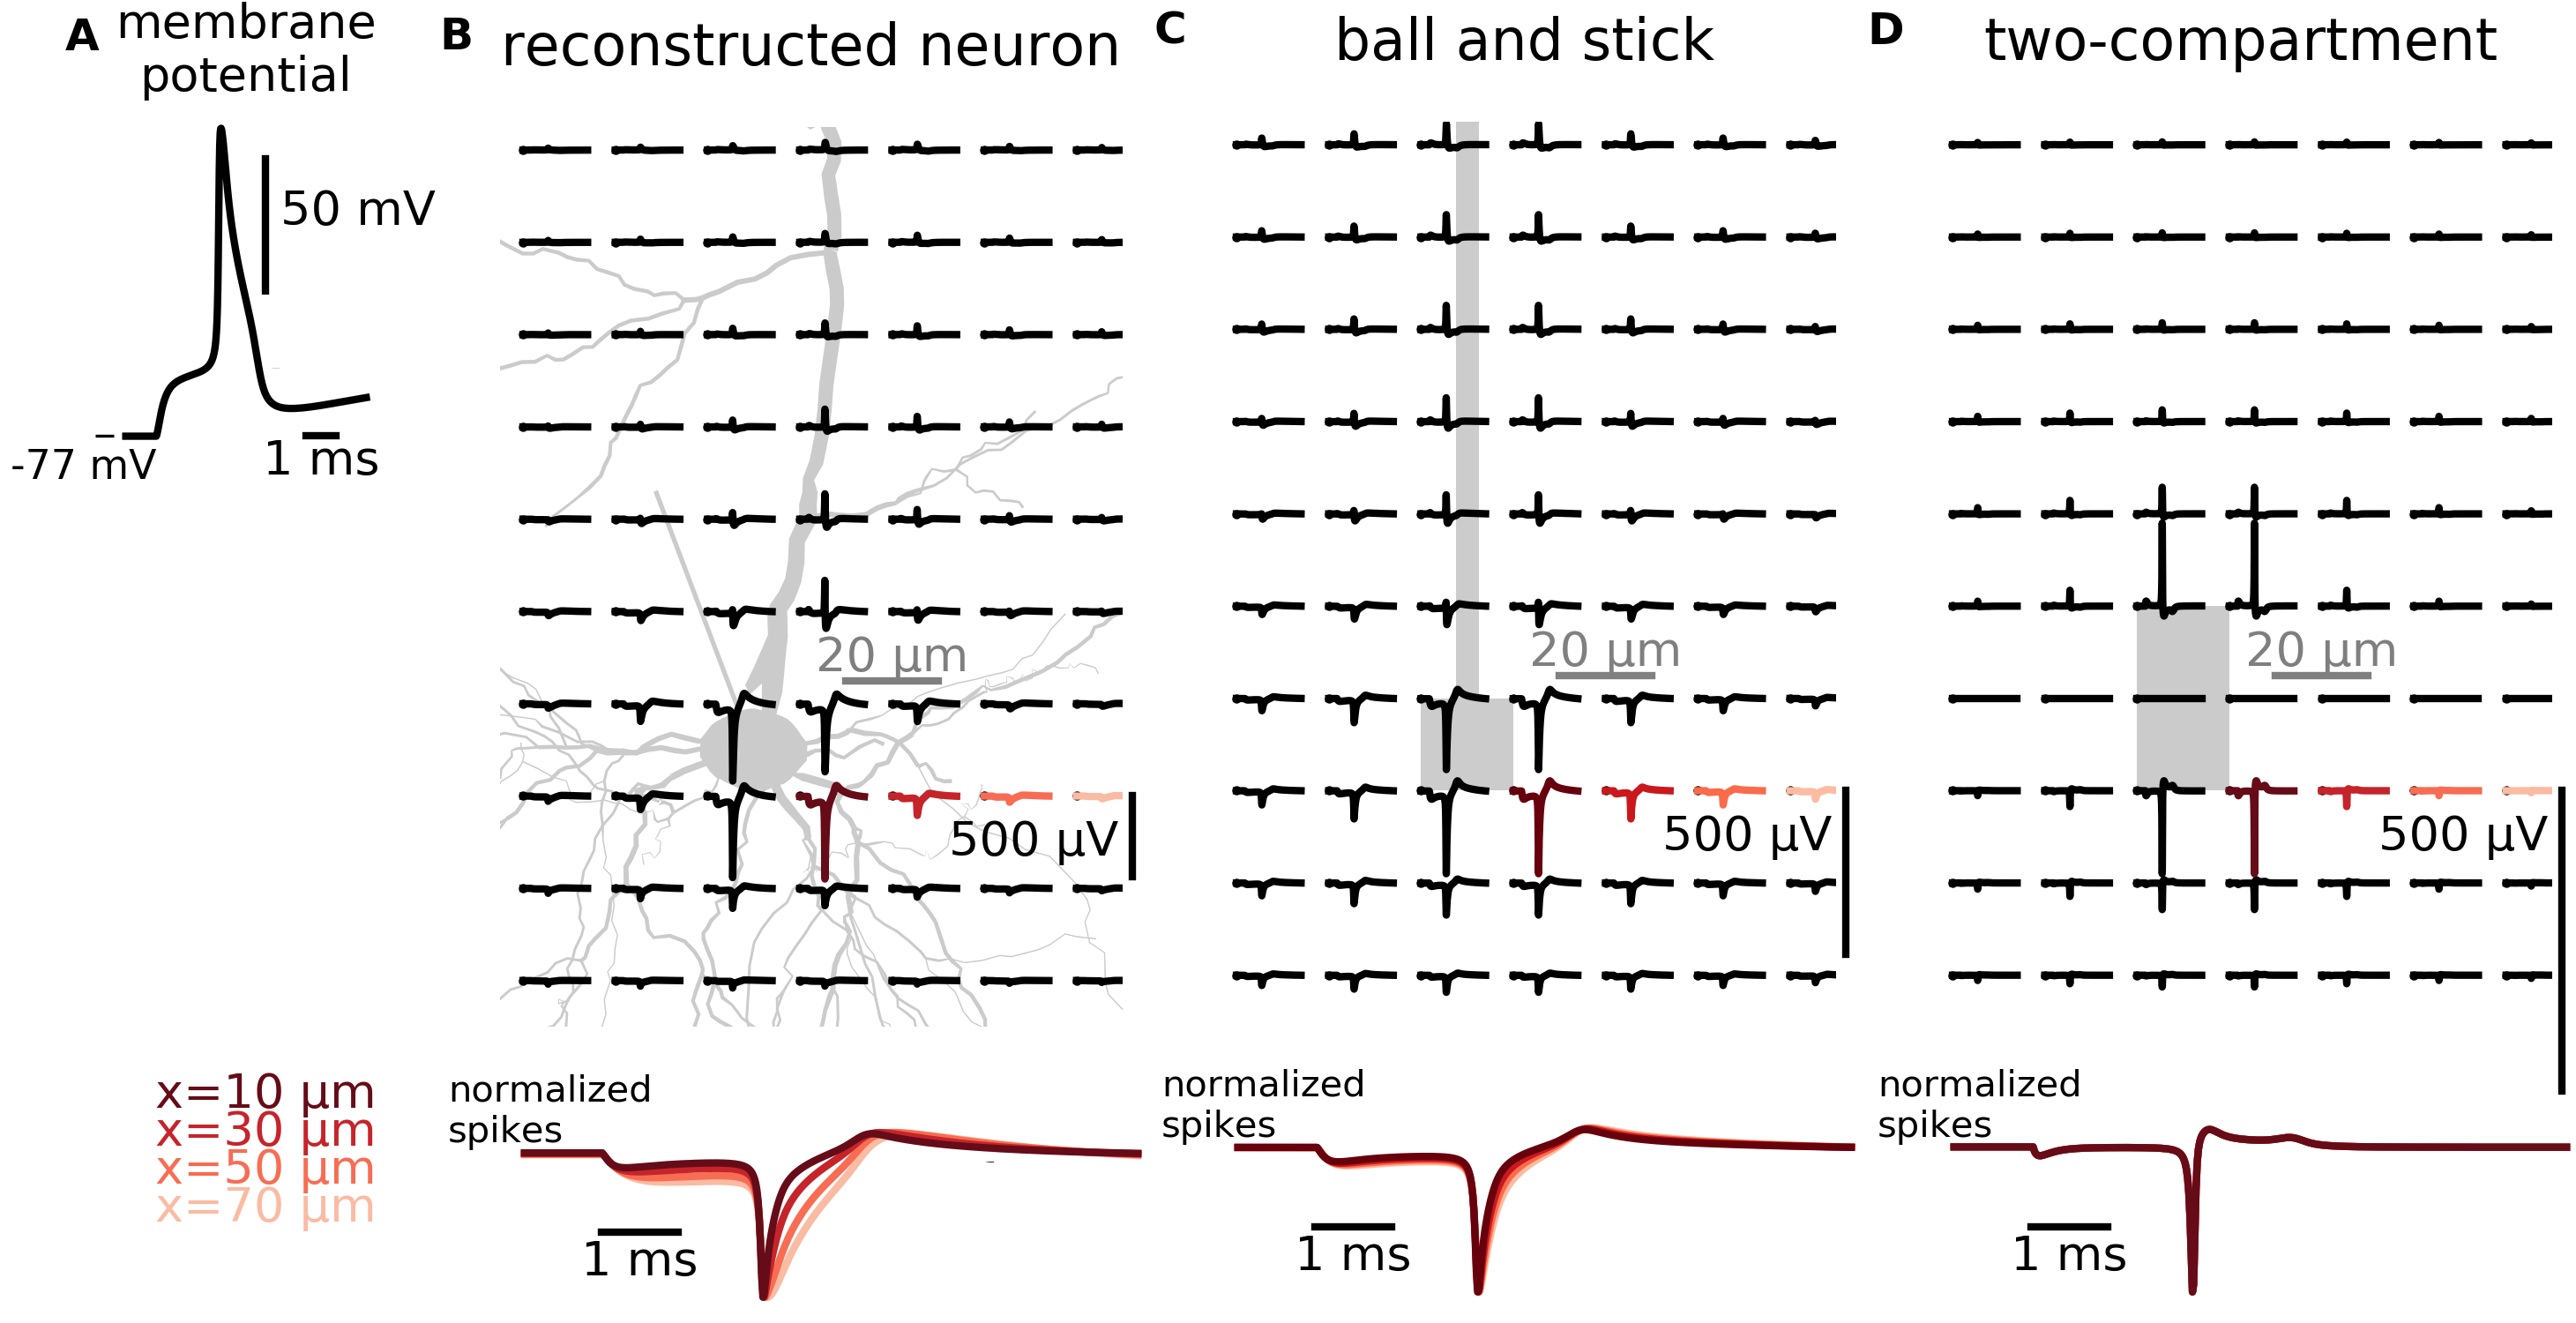
\includegraphics[width=1.2\textwidth]{Figures/Spikes/Spikes-compare_hay_bns_2c_reformat_2}
\end{center}
\caption[]{\textbf{Comparison of spikes from action potential for different neuron models.}
A: Membrane potential during spiking event, generated by injection of synaptic current into the soma of  example Hay-neuron \cite**{Hay2011}. B: Spikes computed at different positions around example Hay-neuron using \gex{Eq. XX} (top). 
C: Spikes computed for example ball-and-stick neuron when imposing the membrane potential in A in the soma of the model neuron (top). Neuron parameters are \gex{XX}. 
D: Spikes computed for example two-compartment neuron when imposing the membrane potential in A in the soma of the model neuron (top). Neuron parameters are \gex{XX}. For panels B--D, spikes shapes at different lateral positions as depicted by colouring, are shown in bottom panels. Spike shapes are normalized to have the same magnitude of the negative peak.
\gen{Lurer paa om panelene kunne blitt finere ved aa bruke et kortere utsnitt langs tidsaksen?}
}
\label{fig:Spikes:DifferentNeuronModels}
\end{figure}

%%%
\subsection{\blue{Spikes from ball-and-stick neuron}}
\label{sec:Spikes:ball-and-stick}
Unlike the two-compartment neuron model, the so-called ball-and-stick neuron model (\fref{sec:Neuron:ball-n-stick}) 
exhibits position dependence of the spike shape (\Fref{fig:Spikes:DifferentNeuronModels}C). 
In this model a dendrite cable `stick' is connected to a point-like soma. 
The position dependence is not as pronounced as for the anatomically detailed multi-compartment neuron model (panel B), 
but the key qualitative feature remains: the spike gets blunter when moving away from the soma. 
In particular, the width of the negative sodium peak is seen to increase with increased lateral distance.
Also, the unrealistically large positive (inverted) spikes seen outside the dendrite of the two-compartment model are absent in the ball-and-stick model, making it in better accordance with predictions from the multi-compartment model.


\section{\blue{Analysis of spike shapes and sizes}}
\gex{
As discussed above, the ball-and-stick neuron reproduces several of the key qualitative features of spikes seen for the anatomically detailed multi-compartmental example neuron, cf. \Fref{fig:Spikes:DifferentNeuronModels}.}
Unlike anatomically detailed multi-compartment neuron models, it is is amenable to analytical mathematical studies. 
\citeasnoun**{Pettersen2008a} took advantage of this and used this model to explore the link between the morphology and electrical properties of neurons and the shape and size of the spike they produce during an action potential. 
\Fref{fig:Spikes:ball-and-stick-results} shows the distance dependence of the spike amplitude and spike width both for a detailed multi-compartmental pyramidal neuron model and ball-and-stick neurons. While the spike width and amplitude of the multi-compartmental neuron are larger than for the two example ball-and-stick neurons (with short and long dendrite sticks \ghtxt{\sout{, respectively}})
\gen{Boer det ikke vaere med "respectively" her da?}\ghnote{Respectively betyr noe ala "in the order mentioned", men paastanden her er rekkefoelge-invariant.}, the shapes of the curves are similar. \ghnote{Kan vi ikke velge parametere slik at amplituden og shapen ligner i de to tilfellene?}  \gen{Jo, det kan sikkert vaere mulig. Dette er klippet rett fra Pettersen2008a.} Note also that the results for a ball-and-stick neuron with an infinitely long dendritic stick is effectively identical to the long-stick results in the figure~\cite**{Pettersen2008}.


%%%%%%%%%%
% Figure: Spike widths and amplitudes
%%%%%%%%%%
%\begin{cnfigure}{Figures/mm/EP-spike-ball-and-stick-results-w100-r150}
\begin{figure}[!ht]
\begin{center}
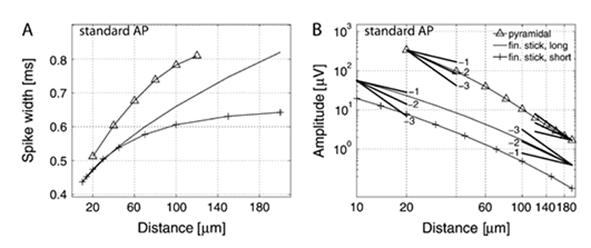
\includegraphics{Figures/Spikes/Spikes-ball-and-stick-results-w100-r150}
\end{center}
\caption[]{
Spike widths (left) and (peak-to-peak) spike amplitudes (right) as a function of distance from soma for a detailed pyramidal cell model (pyramidal) and two types of ball-and-stick models: long, finite ball-and-stick model (fin.~stick, long) with diameter $d=2~\mu$m and length $l=1$~mm and a short, finite ball-and-stick model (fin.~stick, short) with diameter $d=1~\mu$m and length $l=0.2$~mm. The intracellular action potential shown in the inset in the left panel of \Fref{fig:Spikes:ball-and-stick-frequency} was imposed as a voltage-clamp in the soma, and the size and electrical properties of the soma thus did not affect the results. The EP was recorded in the somatic plane normal to the stick/primary apical dendrite. In right panels guidelines illustrating the power-law decays $1/r$ and $1/r^{2}$ have been added. For further details see \citeasnoun**[Figure 6]{Pettersen2008}. \gen{Figure + caption to be updated.}  Adapted from \citeasnoun**{Pettersen2008a}. \gen{Her kunne man jo kjoert ut nye resultater for Hay-modellen, men det er vel like greit aa bare bruke figurene fra Pettersen2008?} \tvnnote{Gaar jo forsaavidt fort aa lage paa nytt, og kan jo vaere fint at det blir en del av koden leserne har tilgjengelig?}
\gen{Enig. I tilfelle maa ogsaa Fig. 8.7 lages paa nytt.} 
}
\label{fig:Spikes:ball-and-stick-results}
%\figpermOurs
\end{figure}
%%%%


%
%%%%%%%%%%%
%% Figure: Neuron models considered in plot of spike widths and amplitudes
%%%%%%%%%%% 
%%\begin{cnfigure}{Figures/mm/EP-spike-ball-and-stick-neuron-models-w43-r300}
%\begin{figure}[!ht]
%\begin{center}
%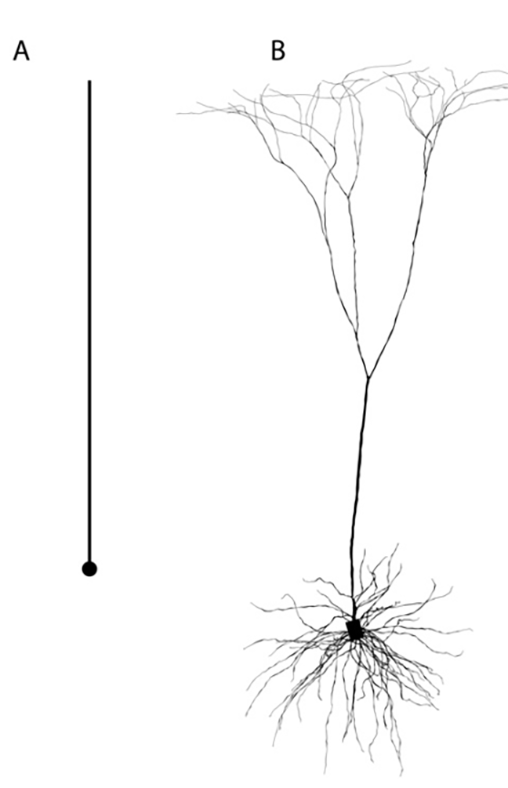
\includegraphics{Figures/Spikes/Spikes-ball-and-stick-neuron-models-w43-r300}
%\end{center}
%\caption[]{\textbf{Neuron models considered in results in \Fref{fig:Spikes:ball-and-stick-results}}. 
%\gen{Mulig vi ikke trenger en slik figur lenger pga Fig 8.3}
%Adapted from \citeasnoun**{Pettersen2008}.
%}
%\label{fig:Spikes:ball-and-stick-neuron-models}
%%\figpermOurs
%\end{figure}

When modeling spikes with the ball-and-stick neuron, one option is to include spike-generating active sodium and potassium conductances in the soma compartment. Another option \ghtxt{(which we will use in all cases studied in this book) is to impose a voltage waveform mimicking a somatic action potential as a boundary condition in the soma end of the dendritic stick. \ghtxt{\sout{This}Both options} will produce an identical pattern of membrane currents returning to the ECS through the dendritic stick. The soma membrane current will due to current conservation be the same as the axial current entering the dendritic stick at the soma end. 

\ghtxt{\sout{The extracellular potential can now be computed using the standard formalism based on the pattern dendritic membrane currents and the soma membrane current Pettersen2008a}} \ghnote{Rar setning. Pattern OF dendritic and somatic membrane currents? Synes ogsaa det var rart aa kalle dette standard formalism da vi ikke har introdusert den tidligere i boka.
Se forslag under. }

\ghtxt{The pattern of dendritic and somatic membrane currents give rise to an extracellular potential
that can be computed with ~\cite**{Pettersen2008a}: }
%
\begin{equation}
  V_\mathrm{e}(z,\rho) = 
  \frac{1}{4 \pi \sigma} \frac{I_\mathrm{soma}}{\sqrt{(z-z_\mathrm{soma})^2+\rho^2}} +
  \frac{1}{4 \pi \sigma} \int_0^l \frac{i_\mathrm{m}(z')~dz'}{\sqrt{(z-z')^2+\rho^2}}.
  \label{eq:Spikes:ball-and-stick-formula}
\end{equation}
Here $\rho$ is the radial distance from the recording point to the dendritic stick axis, and $z_\mathrm{soma}$ 
is the depth position of the soma (see  \Fref{fig:Spikes:ball-and-stick-model-sketch}). 
\ghtxt{\sout{For the present analysis we will use this second option.}}
\ghtxt{We recognize the somatic contribution (first term on the right) as the point-source equation 
(\fref{eq:VC:pointsource2}), while the contribution from the dendritic stick (second term on the right)
is essentially a continuous version of \fref{eq:VC:pointsources}, i.e., a continuum of point sources
distributed along the stick.}
\gen{Sjekk symbolene for soma membranstroem (Ampere) og stick membranstroem (A/m)} 

%

%%%%%%%%%%
% Figure: Spike widths and amplitudes
%%%%%%%%%%
%\begin{cnfigure}{Figures/mm/EP-spike-ball-and-stick-results-w100-r150}
\begin{figure}[!ht]
\begin{center}
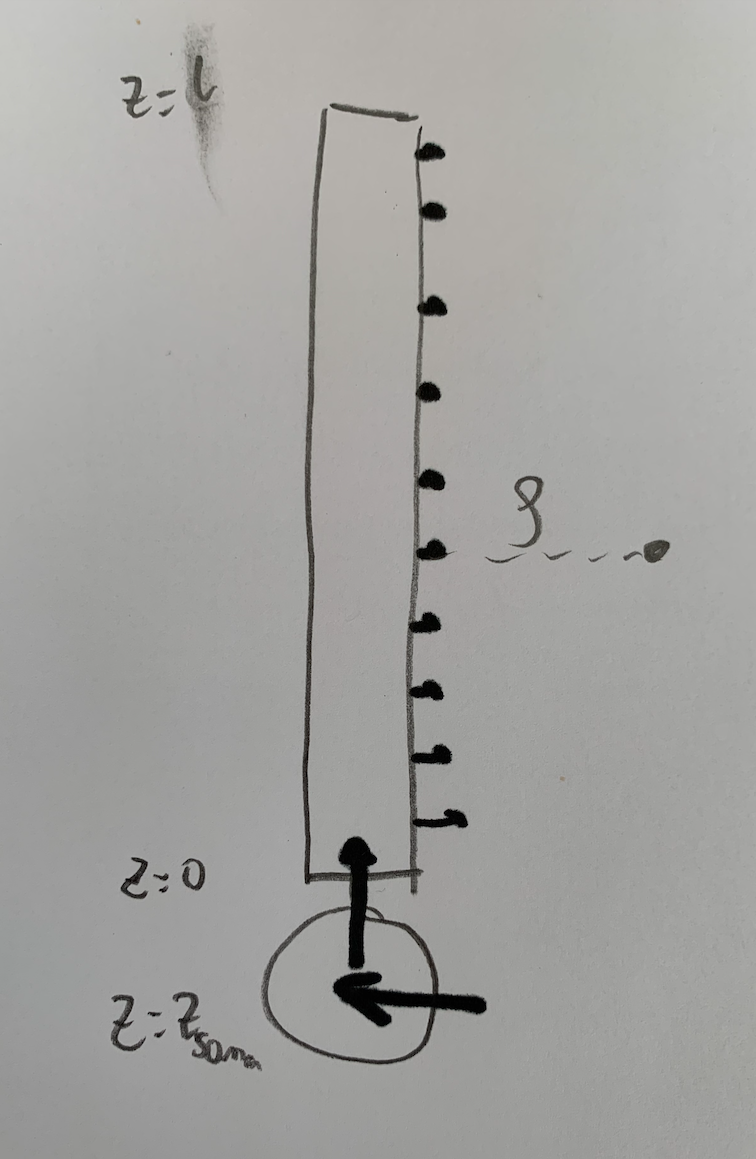
\includegraphics[width=0.6\textwidth]{Figures/Spikes/Spikes-ball-and-stick-model-sketch}
\end{center}
\caption[]{Illustration of ball-and-stick model used in deriving approximate spike formulas.
Arrows illustrate flow of current during the early part of the action potential where the 
inward sodium current dominates.}
\label{fig:Spikes:ball-and-stick-model-sketch}
%\figpermOurs
\end{figure}
%%%%

Since the dendritic stick is passive, its response to imposed currents or voltages is linear.  
It is then convenient to decompose the soma action potential into a Fourier sum of oscillatory components with different 
frequencies and consider each frequency component of the action potential separately. 
Each oscillatory component of the soma action potentials gives an oscillatory axial current entering the stick at the soma end. The spatial pattern of return current along the stick will depend on the frequency of the oscillation 
due to the capacitive properties of the membrane: 
For higher frequencies, the capacitive membrane current will be larger, 
and the membrane effectively more leaky. 
Thus the imposed soma potential will result in dendritic membrane currents returning closer to the soma for higher frequencies, 
as illustrated in the inset in \Fref{fig:Spikes:ball-and-stick-sketch}.  

%%%%%%%%%%
% Figure: Frequency-dependent distribution of return currents
%%%%%%%%%%
%\begin{cnfigure}{Figures/mm/EP-spike-ball-and-stick-sketch-w70-r300}
\begin{figure}[!ht]
\begin{center}
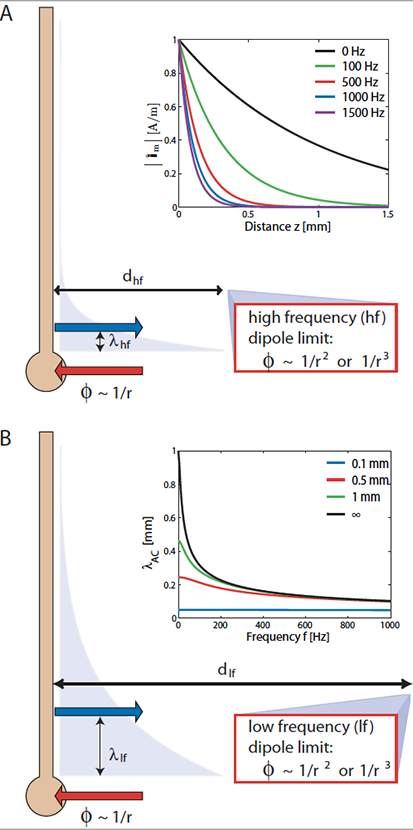
\includegraphics{Figures/Spikes/Spikes-ball-and-stick-sketch-w70-r150}
\end{center}
\caption[]{Illustration of ball-and-stick neuron and its frequency-dependent 
distribution of dendritic return currents following injection of a sinusoidal current into the soma.
The net current entering the soma will enter the dendrite as an axial current, and return to the 
ECS via the dendrite membrane. The inset shows the spatial distribution of this return current
for different frequencies. The higher the frequency, the closer the return currents will be and
the smaller the frequency-dependent length constant $\hat{\lambda}(f)$, reflecting the weighted mean 
of the return-current positions (see sidebox), will be. 
\gen{Figure + caption to be updated.} Adapted from \citeasnoun**{Pettersen2012}.
}
\label{fig:Spikes:ball-and-stick-sketch}
%\figpermOurs
\end{figure}
%

A Fourier sum of a signal such as the soma action potential can be constructed in various ways. The derivations presented below, building on \citeasnoun**{Pettersen2008a}, use the convention that a time signal $S(t)$ can be written as
%%%
\begin{equation}
S(t) = Re \{ \sum_{f}  \hat{S}(f) \exp (j 2 \pi f t) \}
\label{eq:Spikes:Fourier_sum}
\end{equation}
%%%
where $Re\{z\}$ represents the real part of the complex number $z$.  Here $j$ is the unit of imaginary numbers, $f$ is the frequency, and the weight $\hat{S}(f)$ is in general complex. 

\Fref{fig:Spikes:ball-and-stick-frequency} illustrates the Fourier decomposition of the intracellular action potential (membrane potential) and extracellular spike, respectively. In panel B the weight of the different frequency components needed to represent the signals are shown. A key observation here is that unlike for the intracellular action potential, the largest contributions to the extracellular spike, comes from frequencies larger than 100~hertz.
\tvnnote{De er foroevrig betydelig likere i mine simuleringer med Hay modellen, selv om det generelle moensteret vel kanskje er omtrent det samme som her.}


%%%%%%%%%%
% Figure: Action potential and its frequency content
%%%%%%%%%%
%\begin{cnfigure}{Figures/mm/EP-spike-ball-and-stick-frequency-w90-r150}
\begin{figure}[!ht]
\begin{center}
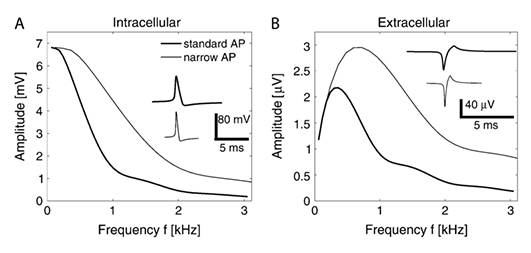
\includegraphics{Figures/Spikes/Spikes-ball-and-stick-frequency-w90-r150}
\end{center}
\caption[]{(A) Action potential used in simulations in \Fref{fig:Spikes:ball-and-stick-results}(inset) 
and its frequency content.
%The intracellular spike width is defined as the
%width of the AP at half amplitude and is 0.55~ms for the standard
%AP, and half the value for the narrow AP. 
(B) Frequency content of example extracellular spike. Inset: Typical spike shape computed a distance $r=10~\si{\micro\metre}$ perpendicular to the dendrite at the level of soma for a ball-and-stick neuron with diameter $d=2~\si{\micro\metre}$ and infinite dendrite length. Here the intracellular action potential in left panel was imposed as a voltage-clamp in the soma.
The extracellular spike width is defined as the width of the negative phase at 25\% of its maximum
amplitude and is 0.44~ms for the example spike. The amplitude (peak-to-peak value) of the spike is $56~\si{\micro\volt}$  
\gen{Figure + caption to be updated. Will only include standard AP in final figure.}  Adapted from \citeasnoun**{Pettersen2008}.}
\gen{Her kunne man jo kjoert ut nye resultater for Hay-modellen, men det er kanskje like greit aa bare bruke figurene fra 
Pettersen2008?} \ghnote{mV/Hz paa y-aksen.}
\label{fig:Spikes:ball-and-stick-frequency}
%\figpermOurs
\end{figure}

%\subsection{Frequency-dependent electrotonic length constant}
%\label{sec:Spikes:Fourier}
%
%For the ball-and-stick neuron, a membrane current entering the soma has to return to ECS through the cable stick, see \Fref{fig:Spikes:ball-and-stick-sketch}. When an oscillating membrane current is entered through the soma, the spatial pattern of return current will depend on the frequency of the oscillation due to the capacitive properties of the membrane: For higher frequencies the capacitive membrane current will be larger, and the 
%membrane effectively more leaky. Thus the injected soma current will return closer to the soma for higher frequencies, 
%as  seen in the inset in \Fref{fig:Spikes:ball-and-stick-sketch}.  

\subsection{\blue{Approximate spike formulas}}
\label{sec:Spikes:approximate}
\gex{
For the ball-and-stick model analytical expressions can be found from \Fref{eq:Spikes:ball-and-stick-formula}
for the extracellular potential generated by an oscillatory voltage imposed in the soma, see \citeasnoun**{Pettersen2008}. The resulting formulas are cumbersome and difficult to interpret. However, some useful insights can be obtained in two limiting cases: the recording being very near to the soma or very far from the soma.}


\subsubsection{Spikes recorded near the soma}
\label{sec:Spikes:near-spikes}
For recording positions $\vec{r}$ very close to the soma, the contribution from the soma current will dominate over the contributions from the dendrite in the sum giving the extracellular potential in \Fref{eq:Spikes:ball-and-stick-formula}. \gex{If we know the amplitude of the oscillatory soma membrane current $|\hat{I}_\mathrm{s}(f)|$,} the amplitude of the predicted oscillating extracellular potential $|\hat{V}_\mathrm{e,near}(f,\vec{r})|$ is approximately given by 
%
\begin{equation}
  |\hat{V}_\mathrm{e,near}(f,\vec{r})| = \frac{|\hat{I}_\mathrm{s}(f)|}{4 \pi \sigma r} .
  \label{eq:Spikes:Ve_near_1}
\end{equation}
%
%where $|\hat{I}_\mathrm{s}(f)|$ is the amplitude of the oscillating current through the soma membrane.
%and also the axial current entering the dendrite from the soma compartment. 
\gex{This oscillating soma membrane current $|\hat{I}_\mathrm{s}(f)|$ is identical to the current entering the dendritic stick, 
and for the relatively high frequencies of most relevance for the spike, it can be shown that the soma current is} related to the soma membrane potential 
$\hat{V}_\mathrm{s}(f)$ through~\cite**{Pettersen2008a}
%
\begin{equation}
  |\hat{I}_\mathrm{s}(f)| =  \frac{\pi^{3/2} d^{3/2}}{\sqrt{2}} \sqrt{ \frac{f c_\mathrm{m}}{r_\mathrm{a}} }  |\hat{V}_\mathrm{s}(f)|\,.
  \label{eq:Spikes:Isoma}
\end{equation}
%
\gex{The amplitude of the contribution to the spike from this oscillatory component} is thus found to be
%
\begin{equation}
  |\hat{V}_\mathrm{e,near}(f,\vec{r})| 
  = \frac{\sqrt{\pi}}{4 \sqrt{2} \sigma}
     \frac{d^{3/2}}{r} 
     \sqrt{ \frac{f c_\mathrm{m}}{r_\mathrm{a}} }  |\hat{V}_\mathrm{s}(f)| 
  \propto \frac{d^{3/2}}{r} \sqrt{ \frac{f c_\mathrm{m}}{r_\mathrm{a}} }  |\hat{V}_\mathrm{s}(f)|. 
  \label{eq:Spikes:Ve_near_2}
\end{equation}
%
%%%%%%%%%%
%However, as shown in XX
%Box~\Fref{mm:box:ball-and-stick-spikes} 
%some useful insights can be obtained in two limiting cases: the recording being very near to the soma or very far from the soma.

%For recording positions very close to the soma, the contribution from the soma current will dominate 
%in the sum in \Fref{XX:equation:Ve-multi-compartment}. In this case the distance from the electrode
%to the return currents in the dendrite will be much larger than the distance to soma. With only the contribution from
%the soma compartment included, the amplitude $|\hat{V}_\mathrm{e,near}(f,\vec{r})|$  
%of the EP signal for each Fourier component with frequency $f$ is found to be
%%
%\begin{equation}
%  |\hat{V}_\mathrm{e,near}(f,\vec{r})| 
%  \propto \frac{d^{3/2}}{r} \sqrt{ \frac{f c_\mathrm{m}}{r_\mathrm{a}} }  |\hat{V}_\mathrm{s}(f)| 
%  \label{eq:Spikes:Ve_near}
%\end{equation}
%%
The suffix `near' is added because this expression only applies in the `near-field' limit, that is, close to the soma.
\tvnnote{Comment on what 'near' means? Up to a few tens of micrometers?} 
$|\hat{V}_\mathrm{s}(f)|$ is the amplitude of Fourier component of the soma membrane potential at the same
frequency (see \Fref{fig:Spikes:ball-and-stick-frequency}). Further, $d$ is the diameter of the dendritic
stick, $c_\mathrm{m}$ is the specific membrane capacitance, and $r_\mathrm{a}$ is the specific axial resistance.  

%One of the predictions from the formula in \Fref{eq:Spikes:Ve_near_2} is that the amplitude of each Fourier component decays
%as $1/r$ when moving away from soma (yet staying within distances where the `near-field' approximation is still applicable).
%Since this applies to all Fourier components which together constitute the action potential, this implies that the amplitude of the 
%spike will decay as $1/r$ in this regime as well.
%\gen{From David Sterratt: Intuition for the relationship witd $d, c_m, f, r_a$.}


\subsubsection{Spikes recorded far away from soma}
\label{sec:Spikes:far-spikes}
For spikes recorded close to the soma, a single membrane current, the soma current, dominates the sum in 
\Fref{eq:Spikes:ball-and-stick-formula}, as we described above. For recording positions far away from the soma, the contribution from return membrane currents must also be included in the sum. For the ball-and-stick neuron, a membrane current entering the soma has to return to ECS through the cable stick, see \Fref{fig:Spikes:ball-and-stick-model-sketch}. When an oscillating
\gex{potential is imposed in the soma,} the spatial pattern of return current will depend on the frequency of the oscillation.
This is an effect of the capacitive properties of the membrane: For higher frequencies the capacitive membrane current will be larger, and the membrane effectively more leaky. Thus the injected soma current will return to the extracellular space closer to the soma for higher frequencies, as  seen in the inset in \Fref{fig:Spikes:ball-and-stick-sketch}.  

An approximate way of including the contribution from \gex{an oscillatory component to the spike} 
from the dendritic return currents is to assume all return currents to leave the dendrite at a single point. 
\gex{The position of this `return-current point' will depend on the frequency of the component.}
Then we are left with a current dipole where the transmembrane current entering at the soma is at all times balanced by an oppositely directed current with the same magnitude leaving at a single point on the dendrite. The current dipole length is then given by the distance between the soma and the dendritic position of the return current, \gex{and we effectively 
have a two-compartment model describing the contribution from this particular oscillatory component of the action potential.} 

As shown in \Fref{fig:Spikes:ball-and-stick-sketch} this current-dipole length will depend on frequency. A natural choice is to choose the dipole length to be equal to the frequency-dependent length constant $\lambda_\mathrm{AC}(f)$ of the stick, where the length constant corresponds to the mean value of the envelope of the sinusoidally varying (normalized) membrane current $\hat{i}_\mathrm{m}$ weighted with distance $z$ from soma, see \Fref{fig:Spikes:ball-and-stick-sketch}. For an infinite dendrite stick this corresponds to
%
\begin{equation}
  \lambda_\mathrm{AC}^\infty(f) = \frac{\int_0^\infty z |\hat{i}_\mathrm{m}| dz}{\int_0^\infty |\hat{i}_\mathrm{m}| dz} 
  \label{eq:Spikes:formula_lambda_ac}
%=  \frac{\sqrt{2}\lambda}{\sqrt{\sqrt{W^2+1}+1}}.
\end{equation}
%
For high frequencies ($f \gg 1/2 \pi r_\mathrm{m} c_\mathrm{m}$) this is after some algebra found to give (see \citeasnoun[Appendix C]{Pettersen2008a} for details)
%
\begin{equation}
 \lambda_\mathrm{AC}^\infty(f) =  \frac{\lambda}{\sqrt{\pi f \tau}} = 
  \frac{1}{2\sqrt{\pi}} \sqrt{\frac{d}{f r_\mathrm{m} c_\mathrm{m}}}
\label{eq:Spikes:approx_lambda_ac}
\end{equation}
%
where $\lambda$ is the cable length constant from Equation~\gex{XX}. The extracellular potential contribution from each frequency component can then be approximated by using the dipolar expression in Equation~\gex{XX}, that is,
%%%
\begin{equation}
  |\hat{V}_\mathrm{e,far}(f,\vec{r})| =  \frac{|p(f) \cos \theta|}{4 \pi \sigma r^2} 
                                            = \frac{| \hat{I}_{s}(f) \lambda_\mathrm{AC}(f) \cos \theta|}{4 \pi \sigma r^2}   
                                                                                        \label{eq:Spikes:Ve_far_1}
\end{equation}
%Chapter~\Fref{XX:chap:XX}
Thus for spikes measured far away from the soma we find 
%  
\begin{equation}
  |\hat{V}_\mathrm{e,far}(f,\vec{r})|  = \frac{1}{8 \sqrt{2} \sigma} d^{2} \frac{1}{r^2  r_\mathrm{a}} 
      |\hat{V}_\mathrm{s}(f) \cos \theta | 
  \propto d^{2} \frac{|\cos \theta|}{r^2  r_\mathrm{a}} |\hat{V}_\mathrm{s}(f)| 
  \label{eq:Spikes:Ve_far_2}
\end{equation}
The suffix `far' is added because this expression only applies in the `far-field' limit, that is, far away from the soma. 
\ehnote{`far-field' limit har vel en noe mer generell definisjon?}
\gen{Etter aa tenkt litt mer tror jeg det er OK aa si far-field limit siden dette dipolleddet vil dominere i denne grensen.}
\ghnote{Skal lambda hete lambda infinity? } \gen{Ja, det var tanken siden vi bruker uttrykket for en uendelig stick}
%
%Equations~(\Fref{eq:Spikes:Ve_near_2}) and (\Fref{Spikes:box:equation:Ve_far_2}) describe how each frequency component of 
%the soma membrane potential  $\hat{V}_\mathrm{s}(f)$ is `translated' into frequency components of the 
%EP spike ($\hat{V}_\mathrm{e,near}(f,\vec{r})$ and $\hat{V}_\mathrm{e,far}(f,\vec{r})$, respectively). 
%%\end{boxfloat}
%%%%%%%%%%%%%%%%%%%%%%%%%%%%%%%%%%%%%%%%%


%An estimate of this length is provided by the 
%frequency-dependent length constant  $\lambda_\mathrm{AC}(f)$  corresponding to the weighted mean of the positions of the return currents along
%the dendrite stick (see Box XX). 
%Then with the use of expression for the EP around a current dipole in 
%\Fref{XX:equation:Ve-dipole-p}:
%%%%
%\begin{equation}
%  |\hat{V}_\mathrm{e,far}(f,\vec{r})|  \propto d^{2} \frac{|\cos \theta| }{r^2  r_\mathrm{a}}  |\hat{V}_\mathrm{s}(f)| 
%  \label{eq:Spikes:Ve_far}
%\end{equation}
%%%%



%A first observation from this formula is that the EP is no longer radially symmetric, and depends both on the radial distance $r$ from the neuron and  the angle $\theta$ with the dipole axis, that is, the direction of the dendritic stick.
%The amplitude will be largest above and below the neuron where $\theta=0^\circ$ and $\theta=180^\circ$, respectively. In the sideways direction 
%($\theta \sim 90^\circ$) the EP will be much smaller, as is characteristic for spatial pattern of potentials around a current
%dipole as illustrated in \Fref{fig:Spikes:TwoCompartment}. A qualitatively similar dipolar pattern, although not so distinct,
%is also seen for the spike generated by the biophysically detailed multi-compartment neuron in \Fref{fig:Spikes:DifferentNeuronModels}.


%Another difference of this far-field expression with the near-field expression in \Fref{eq:Spikes:Ve_near}, is that the
%amplitude decays as $1/r^2$, characteristic for potentials around dipolar sources, rather than $1/r$ which is characteristic for potentials around 
%a single source. This transition from a $1/r$ `monopolar' regime to a $1/r^2$ dipolar regime is indeed observed in
%the spike-amplitude panel in \Fref{fig:Spikes:ball-and-stick-results}.

\subsection{\blue{Spike amplitude dependence on distance}}


A prediction from the near-field formula in \Fref{eq:Spikes:Ve_near_2} is that the amplitude of each Fourier component decays as $1/r$ when moving away from the soma, as long as the position remains within distances where the `near-field' approximation still applies. Since this applies to all frequency components which together constitute the action potential, this implies that the amplitude of the spike will decay as $1/r$ in this regime as well. 

Far away, the far-field formula \Fref{eq:Spikes:Ve_far_2} implies that the spike amplitude depends not only on the radial distance $r$ from the neuron, but also the angle $\theta$ with the dipole axis, the direction of the dendritic stick. The amplitude will be largest above and below the neuron where $\theta=0^\circ$ and $\theta=180^\circ$, respectively. In the sideways direction ($\theta \sim 90^\circ$) the spike will be much smaller, as is characteristic for spatial patterns of potentials around a current dipole as illustrated in \Fref{fig:Spikes:DifferentNeuronModels}D. A qualitatively similar dipolar pattern, although not so distinct, is also seen for the spike generated by the biophysically detailed multi-compartment neuron in 
\Fref{fig:Spikes:DifferentNeuronModels}.
Another difference of this far-field expression with the near-field expression in \Fref{eq:Spikes:Ve_near_2}, is that the
amplitude decays as $1/r^2$, characteristic for potentials around dipolar sources, rather than $1/r$ which is characteristic for potentials around a single source. 
\gen{Dette er litt komplisert aa sammenligne med eksisterende resultater fra detaljerte nevronmodeller (Pettersen2008,Hagen2015) fordi disse resultatene er basert paa forflytning horisontalt utfra soma, noen som gjoer at en forventer at det gaar som 1/r$^3$. Vet ikke om vi trenger aa komme inn paa dette...} 

%This transition from a $1/r$ `monopolar' regime to a $1/r^2$ dipolar regime was also found in model studies with biophysically detailed 
%neurons \cite[Fig.~X]{Pettersen2008}.
%\todo{Connect to Figure :EP-spike-ball-and-stick-results}

An overall observation is that the spike is quite local, with the amplitude of the spike decaying rapidly with distance from the neuronal soma. For the pyramidal neuron considered in Figure~XX, for example, the spike amplitude decays from about
300 microvolts a distance 20 micrometers from the soma centre to only about 10 microvolts a
distance 100 micrometers away. \gen{Update when new figures are added} This rapid decay eases the interpretation of recorded spikes, since it implies that in practice an electrode contact will only pick up spikes from neurons with somas positioned within a radius of some tens of micrometers.
%\todo{GTE: Rewrite this to compare with our own figure spikes around multicompartmental model + refer to Pettersen2008}  

%\paragraph{Spike amplitude dependence on neuronal parameters}
\subsection{\blue{Spike amplitude dependence on neuronal parameters}}
The spike amplitude is proportional to $d^{2}$ far away from the soma  (\Fref{eq:Spikes:Ve_far_2}) and to $d^{3/2}$ close to the soma (\Fref{eq:Spikes:Ve_near_2}),
where $d$ is the diameter of the dendritic stick diameter. This implies that far away from the soma the spike amplitude is proportional to  the cross-sectional area of the dendrite. Close to the soma, the spike amplitude also increases with dendrite diameter, but slightly less so.

Another observation is that the spike amplitude is independent of the membrane resistance $r_\mathrm{m}$ of the dendrite. This reflects that the frequencies dominating the spike are so high that the ionic membrane current, governed by $r_\mathrm{m}$, is much smaller than the capacitive membrane current, governed by membrane capacitance $c_\mathrm{m}$.  Thus the spatial distribution of the return current along the dendrite will depend only on the capacitive current. This dependence is seen through the presence of  $c_\mathrm{m}$ in the near-field formula in \Fref{eq:Spikes:Ve_far_2}. Note that in the far-field formula \Fref{eq:Spikes:Ve_far_2},  $c_\mathrm{m}$ is absent due to cancellation with another factor containing $c_\mathrm{m}$ in the mathematical derivation, cf. \citeasnoun[Equation 23]{Pettersen2008}.)

In \Fref{eq:Spikes:Ve_near_2} and \Fref{eq:Spikes:Ve_far_2}, the spike amplitude is reduced when the 
axial resistance $r_\mathrm{a}$ in the dendrites is increased. This reflects that an increased axial resistance implies that the current entering the soma during the first phase of an action potential will return closer to the soma. This implies shorter distances on average between the sink (soma) and the sources, where the current return to the ECS, and thus a smaller current dipole and a smaller spike.


\subsection{\blue{Spike shape dependence on distance}}
The near-field and far-field formulae in \Fref{eq:Spikes:Ve_near_2} and \Fref{eq:Spikes:Ve_far_2} respectively also give qualitative insights regarding the shape of the spike. In the near-field expression, the high-frequency components of the spike is amplified compared to the low-frequency components, with $\hat{V}_\mathrm{e,near}(f,r) \propto \sqrt{f}$.
Thus close to the soma the spike is observed to be sharper than the intracellular action potential,
as observed in the insets in Figure~\gex{XX}. \gen{If we include such in new figures.} 
In the far-field regime there is no such high-frequency amplification ($\hat{V}_\mathrm{e,near}(f,r) \propto f^0 \sim 1$).
As a consequence, spikes measured far away from the soma will have less high-frequency content than those measured close to soma.
Thus the far-away spikes will be blunter and have larger spike widths as seen in the spike-width panel of 
\Fref{fig:Spikes:ball-and-stick-results}.

At times, the time-derivative of the membrane potential has been used as a proxy for the shape of the extracellular spike.
This would correspond to  $\hat{V}_\mathrm{e}(f) \propto f$ as a time derivation of a Fourier component   
$\exp (j 2 \pi f t)$  is proportional to $f \exp (j 2 \pi f t)$, cf. Equation \Fref{eq:Spikes:Fourier_sum}. This relationship predicts a higher weighting of the high-frequency components, and thus a sharper spike shape, than the  prediction $\hat{V}_\mathrm{e}(f) \propto \sqrt{f}$ for the ball-and-stick neuron in the near-field limit. For the example in \Fref{fig:Spikes:Henze} we observe that the time-derivative of the membrane potentials predicts a too narrow spike shape compared to the experimental data.
\gen{Kunne vi lagd en versjon av Figur 8.1 hvor vi har med $\sqrt{f}$-prediksjonen?} 


%\paragraph{Generalisation of findings to other neuron models}
\subsection{\blue{Generalisation of findings to other neuron morphologies}}
While the formulae above were derived for a neuron model with a single passive dendritic stick, similar expressions can be derived for more complex neural morphologies where several passive sticks protrude from the soma, see \citeasnoun**{Pettersen2008}. The main conclusions above hold also for these `ball-and-sticks' neuron models, in particular that spike widths always increase with distance and that the amplitude of a spike is proportional to $d^{k}$ where $k\sim1.5-2$. For neurons with many dendrites attached to the soma, the contributions to the spike amplitude roughly add up. A simple rule of thumb is that a neuron's spike amplitude is roughly proportional to the sum of the cross-sectional areas for all dendrite branches attached directly onto the soma. Neurons with many thick dendritic branches attached to the soma will thus generate the largest spikes. See~\citeasnoun**{Pettersen2008} for further discussion.
\gen{Kunne eventuelt aa vise noen resultater fra Jorgens thesis her}
\tvnnote{Foeler dette er litt lite testet enn saa lenge til aa ha med i bok? Maa i minste fall gjennskape resultatene, men kan godt gjoere det om du vil :-)}
\gen{Vi kan tenke paa, men jeg synes en del av funnene hans var veldig interessante.}


%\subsection{Insights from spike near- and far-field expressions}
%
%There are several qualitative insights regarding the sizes and widths of spikes that can 
%be found from the near-field and far-field formulae in Equations~\Fref{eq:Spikes:Ve_near_2} and 
%\Fref{eq:Spikes:Ve_far_2}. One relates directly to the shape of the spike:
%in the near-field expression, the high-frequency components of the spike is amplified 
%compared to the low-frequency components, that is, $\hat{V}_\mathrm{e,near}(f,r) \propto \sqrt{f}$.
%Thus close to the soma the spike is observed to be sharper than the intracellular action potential
%as observed in the insets in \Fref{fig:Spikes:ball-and-stick-frequency}. 
%In the far-field regime there is no such high-frequency amplification ($\hat{V}_\mathrm{e,near}(f,r) \propto f^0 \sim 1$).
%As a consequence, spikes measured far away from the soma will have less high-frequency content than those measured close to soma.
%Thus the far-away spikes will be blunter and have larger spike widths as seen in the spike-width panel of 
%\Fref{fig:Spikes:ball-and-stick-results}.
%
%The spike amplitude is proportional to $d^{2}$ far away from the soma and $d^{3/2}$ close to the soma,
%where $d$ is the diameter of the dendritic stick diameter.
%This implies that far-way from the soma the spike amplitude is proportional to the cross-sectional area of the dendrite.
%Close to the soma, the spike amplitude also increases with dendrite diameter, but not so prominently as far away.
%Another observation is that the spike amplitude is independent of the membrane resistance $r_\mathrm{m}$ of the dendrite; only the membrane 
%capacitance $c_\mathrm{m}$ and the axial resistance $r_\mathrm{a}$ matter, 
%This reflects that the frequencies dominating the spike are so high that the capacitive membrane current 
%(governed by $c_\mathrm{m}$) is much larger than the ionic membrane current  (governed by $r_\mathrm{m}$). 
%%\todo{DCS: I'm wondering if we need more details on frequency-dependent cable theory, beyond Eq. 5.11.}
%
%An overall observation is that the spike is quite local, that is, the amplitude of the spike decays rapidly with distance from the neuron soma. For the pyramidal neuron considered in 
%\Fref{fig:Spikes:ball-and-stick-results}, for example, the spike amplitude decays from being about
%300 microvolts a distance 20 micrometers from the soma center to being only about 10 microvolts a
%distance 100 micrometers away. This rapid decay eases the interpretation of recorded spikes, since it implies
%that in practice an electrode contact will only pick up spikes from neurons with somas positioned within a radius of some tens of micrometers.
%
%\gen{Add tekst on generalizability to more complicated models: ball-and-star ,,,}

%%%%%%%%%%%
%% Box: Ball-and-stick model for spikes
%%%%%%%%%%%
%%\begin{boxfloat}{Ball-and-stick model for spikes}
%%  \label{mm:box:ball-and-stick-spikes}  
%\subsection{\red{Box: Ball-and-stick model for spikes}}
%\gen{This was a box in the Sterratt chapter}
%%
%For recording positions further away from the soma, the contribution from return membrane currents must be taken into
%account in the sum in \Fref{XX:equation:Ve-multi-compartment}. 

\section{\blue{Soma spikes initiated in the axon}}
In the investigations of the spike generated by the ball-and-stick neuron above, we assumed that the action potential is generated \ghtxt{\sout{by active conductances}} \ghnote{Vi brukte vel en injisert stroem som representerte dette, og hadde ikke med noen aktive konduktanser?} \gen{Nei, men det ligger jo implisitt.}
in the soma  and that the spike is generated by a current dipole reflecting the distribution of return currents in the dendritic stick. However, in some neurons the action potential is initiated some distance away from the soma along the axon initial segment (AIS)\cite**{Goethals2020}. This will in turn ignite the full soma action potential. In this initial phase of the action potential there will thus be a current dipole where current enters the neuron at AIS and leave through the soma. 

In this scenario there will expectedly be a short-lasting somatic source prior to the longer-lasting somatic sink setting up the characteristic strong negative sodium peak. Model simulations have indeed confirmed that this is feasible and that a small and narrow positive peak can be seen prior to the negative sodium peak for recording close to the soma~\cite**{Telenczuk2018}.
Interestingly, detailed experimental studies of the shape and amplitude of extracellular spikes recorded simultaneously around the soma and along the axon has now become possible by means of high-density microelectrode arrays (HD-MEAs)~\cite**{Emmenegger2019}.
\gen{Comment on axon-representations in Hay-model and Mainen-model.} 
\ehnote{Hay-modellen har ikke et realistisk axon. APs er generert i soma, ikke i akson-stumpen} 


\section{\blue{Spikes in neurons with active dendrites}} 
\gen{This text is adapted from Pettersen2012. Should we add something, for example, a figure?}
In the above investigation of the ball-and-stick neuron, the assumption of an electrically passive dendritic stick was
essential. This assumption made the problem of relating intracellular potentials recorded in the soma to extracellular potentials recorded outside the neuron \emph{linear} and essentially independent of the detailed shape of the intracellular action potential:
the shape of the intracellular action potential only affected the weight of each frequency component in the Fourier sum.
Thus the above analytical insights apply in principle to all intracellular action-potential waveforms.

However, real neurons have active conductances also in the dendrites \cite**{Stuart2007}, making 
the problem nonlinear. The assumption of independent frequency component then no longer holds, and 
instead one has to resort to numerical investigations using the general formula in Equation \gex{XX} where
all active conductances are included explicitly. 

Using this scheme, Gold and coworkers \cite**{Gold2006,Gold2007} performed thorough investigations of the extracellular signatures of spikes from pyramidal neurons in hippocampus CA1 where active dendritic conductances were included in the model. Their results were in qualitative agreement with many of the observations seen above 
for neurons with passive dendrites: (i) the spike width was seen to increase with distance from the soma (cf.~Fig.~5A in Ref.~\citeasnoun**{Gold2006}), (ii) the spike amplitude was seen to decay with distance from the soma with a power between 1 and 2 for distances less than 50 $\mu$m (cf.~Fig.~14 in 
Ref.~\citeasnoun**{Gold2006}), and (iii) the spike amplitude was also seen to change significantly with varying axial resistance $r_\mathrm{a}$ and capacitance $c_\mathrm{m}$, but not so much with varying membrane resistance \cite**{Gold2007}. They also found that extracellular waveforms provide tight constraints on some of the neuronal model parameters, suggesting that extracellular spikes could be useful for constraining compartmental models.

\section{\blue{Axonal spikes}}

The focus in this chapter is on somatic spikes, that is, spikes where the dominating membrane currents setting up the spike during an action potential are in the soma. However, action potentials also propagate along the axons towards other neurons, 
and the associated axonal membrane currents will also generate extracellular potentials, that is, \emph{axonal spikes}.

For two reasons such axonal spikes are often assumed to be small, at least much smaller than somatic spikes.
For one, the diameters of axons are typically less than a micrometer in mammalian brains. This implies a small surface area compared to the surface area of somas, and thus in turn smaller membrane currents and generated spikes. The second reason is that an action potential travelling down an axonal cable do not generate a clear dipolar extracellular potential around the axon.Rather, the potential is more resembling that generated by two opposing dipolar sources largely canceling each other and
effectively generating a much smaller \emph{quadrupolar} extracellular potential around the axon~\cite**{Plonsey1977}.
A thorough exposition of this effect is given in \citeasnoun**[Ch. 8]{Plonsey2007}.

However, axons generally branch out to make many synapses with other neurons, and around such branching points the amplitude of axonal spikes may be much larger. \citeasnoun**{McColgan2017} explored this effect in detail, and key findings from this study is shown in \Fref{fig:Spikes:AxonalSpikes}. Comparison of panels A--D shows that the amplitude of the axonal spike can be strongly boosted when a single axonal cable branches into numerous cables. In real brains one often has synaptic terminal zones where many axons branch of and terminate within a confined region of space. Panel E shows that in this case many action potentials in several axons arriving simultaneously in the terminal zone, may give a sizable net axonal spike. In this case, axonal spikes can and have been be used as a measure of synaptic inputs onto neuronal populations like, for example, in the barn owl auditory brainstem~\cite**{Kuokkanen2018}.


%%%%%%%%%%
% Figure: Axonal spikes
%%%%%%%%%%
%\begin{cnfigure}{Figures/mm/EP-spike-ball-and-stick-sketch-w70-r300}
\begin{figure}[!ht]
\begin{center}
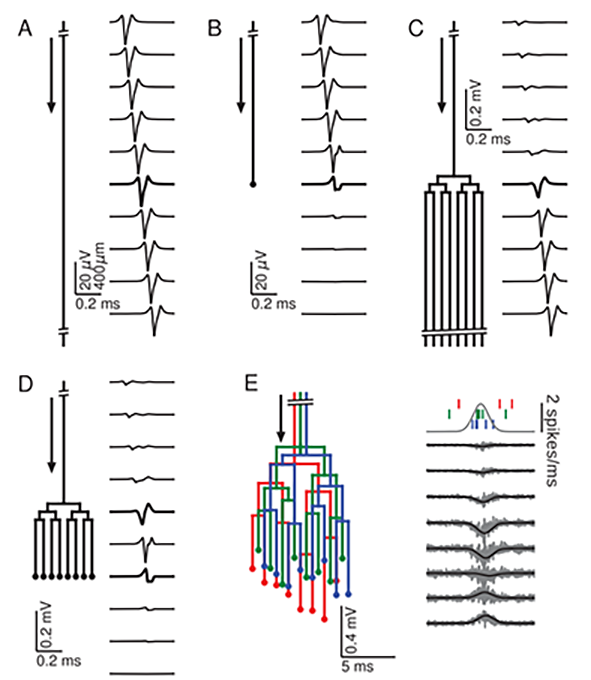
\includegraphics[width=0.7\textwidth]{Figures/Spikes/Spikes-AxonalSpikes-w100-r150}
\end{center}
\caption[]{
Text from McColgan2017: Relationship between axon morphology and extracellular potential. Multi-compartment simulations of action potentials traveling along axons with varying morphologies, as indicated by the diagram on the left-hand side of each subfigure. Action potential propagation direction indicated by arrow. Waveforms, shown on the right- hand side of each subfigure, were recorded at a horizontal distance of 150 mm from the axons. The vertical depth is indicated by the plot position, spaced by 400 mm. Horizontal plot location and distances between axons are for illustration only, all axons were simulated to lie on a straight line. (A) Action potential in a quasi-infinitely long, straight axon. (B) Terminating axon. Action potential waveform closest to the termination thickened for emphasis. (C) Branching axon. The axon branches multiple times within of 200 mm. Thicker waveform at the center of the bifurcation zone. (D) Combined bifurcations and terminations. Note the larger voltage scales in C and D, which correspond to the different number of fibers. (E) Response in a population of 100 randomized morphologies, three of which are shown schematically (colored). Activity consists of spontaneous background activity (100 spikes/s) superimposed with a brief Gaussian pulse of heightened spike rate (2000 spikes/s). Spike rate and example spike times for the three morphologies are shown at the top. Right: gray lines show activity of full population averaged over 40 trials, while the black lines show the low-pass (<1 kHz) component. Note that the time and voltage scales are different from A-D. In all graphs, spatial scales are the same, as indicated by the scale bar in A. 
\gen{Figure + caption to be updated.} Adapted from \citeasnoun**{McColgan2017}.
}
\label{fig:Spikes:AxonalSpikes}
%\figpermOurs
\end{figure}
%


\section{\blue{Effects of measurement device on spike recordings}}
In the above examples we have assumed an infinite volume conductor, that is, the extracellular conductivity has been assumed to be the same everywhere. We have also employed the point-electrode approximation, that is, the recording electrode has been assumed  to record the potential at one particular position in space (\Fref{sec:VC:point-electrode}). Also it has been assumed to faithfully record the extracellular potential without disturbing the potentials around the neuron in any way.  As discussed in \Fref{sec:VC:electrodes}, however, real recording devices will in general affect the measured potentials in several ways.  

\subsection{\blue{Physical sizes of contacts and shafts of recording electrode}}
\label{sec:Spikes:electrode_size}
Most electrodes presently used for extracellular recordings inside the brain consist of electrode contacts made of
highly conductive materials embedded in an electrically insulating electrode shaft. The amplitudes and shapes of 
recorded spikes are affected by the size of the electrode contacts, and as discussed in \Fref{sec:VC:disc-electrode}
this effect can be modelled by use of the disc-electrode approximation. In this approximation the spike potential is computed
by averaging results from using the point approximation across the surface of the electrode, and it is thus straightforward to implement. An example of its use is provided by \Fref{fig:Spikes:electrode_size} showing spikes recorded with circular electrodes of different radii. A key observation is that the spike amplitude is seen to be reduced with increasing contact sizes (panel B). The spikes shape is also affected as the averaging of the potentials across the contact surface will reduce high-frequency components of the spike (panel C).

%%%
\begin{figure}[!ht]
\begin{center}
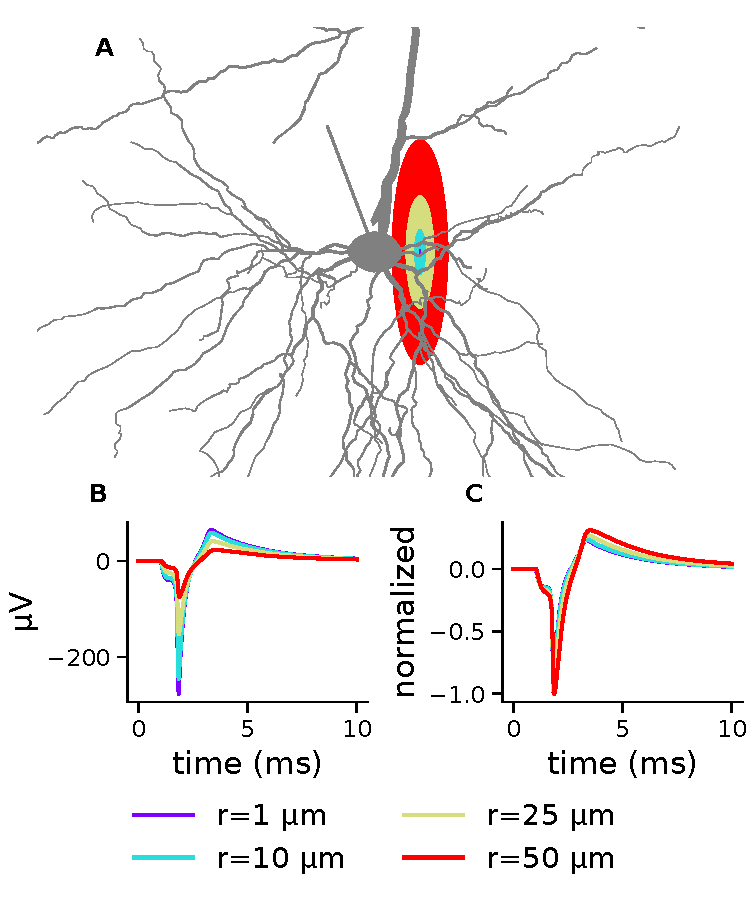
\includegraphics[width=0.6\textwidth]{Figures/Spikes/Spikes-fig_elec_size_effect.pdf}
\end{center}
\caption[]{\textbf{Effect of electrode size.}Bigger recording electrodes can cause smaller and broader EAPs.  \ghnote{Flott. Kursivere $r$? Forklare simuleringen?}
\gen{Veldig fin figur, som kanskje kan passe enda bedre her enn i VC-kapitlet. Hva tenker dere?}}
\ghnote{Ja, siden den fokuserer paa spikes, saa. Skal se hva som trengs i VC naar jeg tar fatt paa det i neste runde.}
\label{fig:Spikes:electrode_size}
\end{figure}
%%%

\gex{The insulating electrode shaft in multicontact electrodes may have a substantial effect on the recorded potentials. 
Detailed studies of this requires comprehensive numerical investigations by use of FEM modeling. Such studies have shown that the signal from neurons placed close to the shaft on the contact side may be amplified, while signals
from neurons positioned close to the back side of the shaft may be dampened~\cite**{Mechler2011,Mechler2012,Buccino2019}. }


\subsection{\blue{Microelectrode arrays (MEAs)}}
Spikes are not only recorded in living brains. In \emph{in vitro} recordings, small slices of excised brain tissue are
placed in suitably designed dishes where physiological properties of cells and networks can be probed in detail for hours.
In so-called \emph{microelectrode arrays (MEAs)}, the bottom of the device is covered by a grid of electrode
contacts which record electrical signals generated by the neurons above. The brain slice and the MEA are both
covered with a liquid, typically saline, to protect the cells from drying out and keep them alive for the duration of the experiment, see \Fref{fig:Spikes:MEA-setup}.

%%%
\begin{figure}[!ht]
\begin{center}
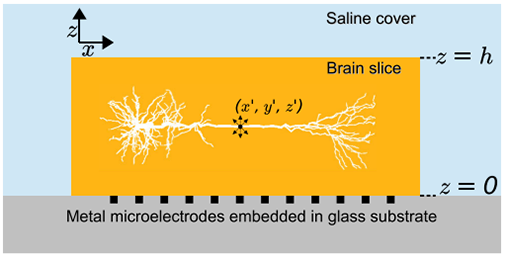
\includegraphics[width=0.7\textwidth]{Figures/Spikes/Spikes-MEA-1-w43-r300}
\end{center}
\caption[]{\textbf{MEA-setup.}
Figure is adapted from \citeasnoun**{Ness2015}.}
\label{fig:Spikes:MEA-setup}
\end{figure}
%%%

In MEAs the electrode contacts are embedded in an insulating glass plate with very 
low electrical conductivity, while the covering liquid typically has a higher electrical conductivity than the brain slice it covers. In this setup the extracellular conductivity around the signal-generating neurons will not be constant as assumed above for the \textit{in vivo} recordings, and this will affect the amplitude and shape of the recorded spikes. 

In general, FEM modeling will be required to solve the forward-modeling for situations such as this where
the the conductivity $\sigma$ varies with position. However, if we assume that the MEA substrate, slice and saline
all extend infinitely in the lateral directions so that $\sigma$ can be assumed to only have planar step-wise discontinuities, 
formulas analogous to \Fref{eq:XX:Vr} can be derived by use of the \emph{method of images} from electrostatics. \gen{Referer til section i VC.}


%%%
\begin{figure}[!ht]
\begin{center}
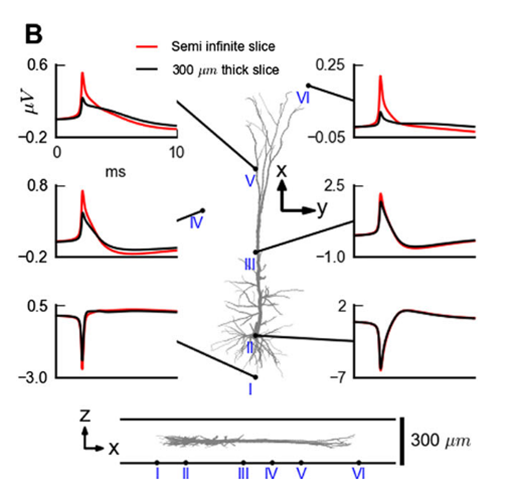
\includegraphics[width=0.8\textwidth]{Figures/Spikes/Spikes-MEA-2-w43-r300}
\end{center}
\caption[]{\textbf{MEA-spikes.}
Figure is adapted from \citeasnoun**{Ness2015}.}
\label{fig:Spikes:MEA-spikes}
\end{figure}
%%%

An example result is shown in \Fref{fig:Spikes:MEA-spikes}. The largest effect on the spike from the measurement device comes from the insulating glass substrate which roughly doubles the amplitude of the recorded spikes, \gex{but this effect is not illustrated in the figure. Rather, the figure illustrates the effect of having a highly conductive saline layer covering the brain slice. Specifically, the saline reduces the size of the spike compared to the hypothetical situation where the saline had the same value of the electrical conductivity as the less conductive brain slice (`semi-infinite slice').}
\gen{Mulig vi boer bruke andre labels paa de to situasjonene i figuren.}

\section{\blue{Multi-unit activity (MUA)}}
In general, a recording contact will pick up spikes from several neurons positioned in its vicinity, that is, from `multiple units'.
The term \emph{multi-unit activity (MUA)} refers to this total spiking activity seen in the high-frequency part of recorded extracellular potentials. 

%%%
\begin{figure}[!ht]
\begin{center}
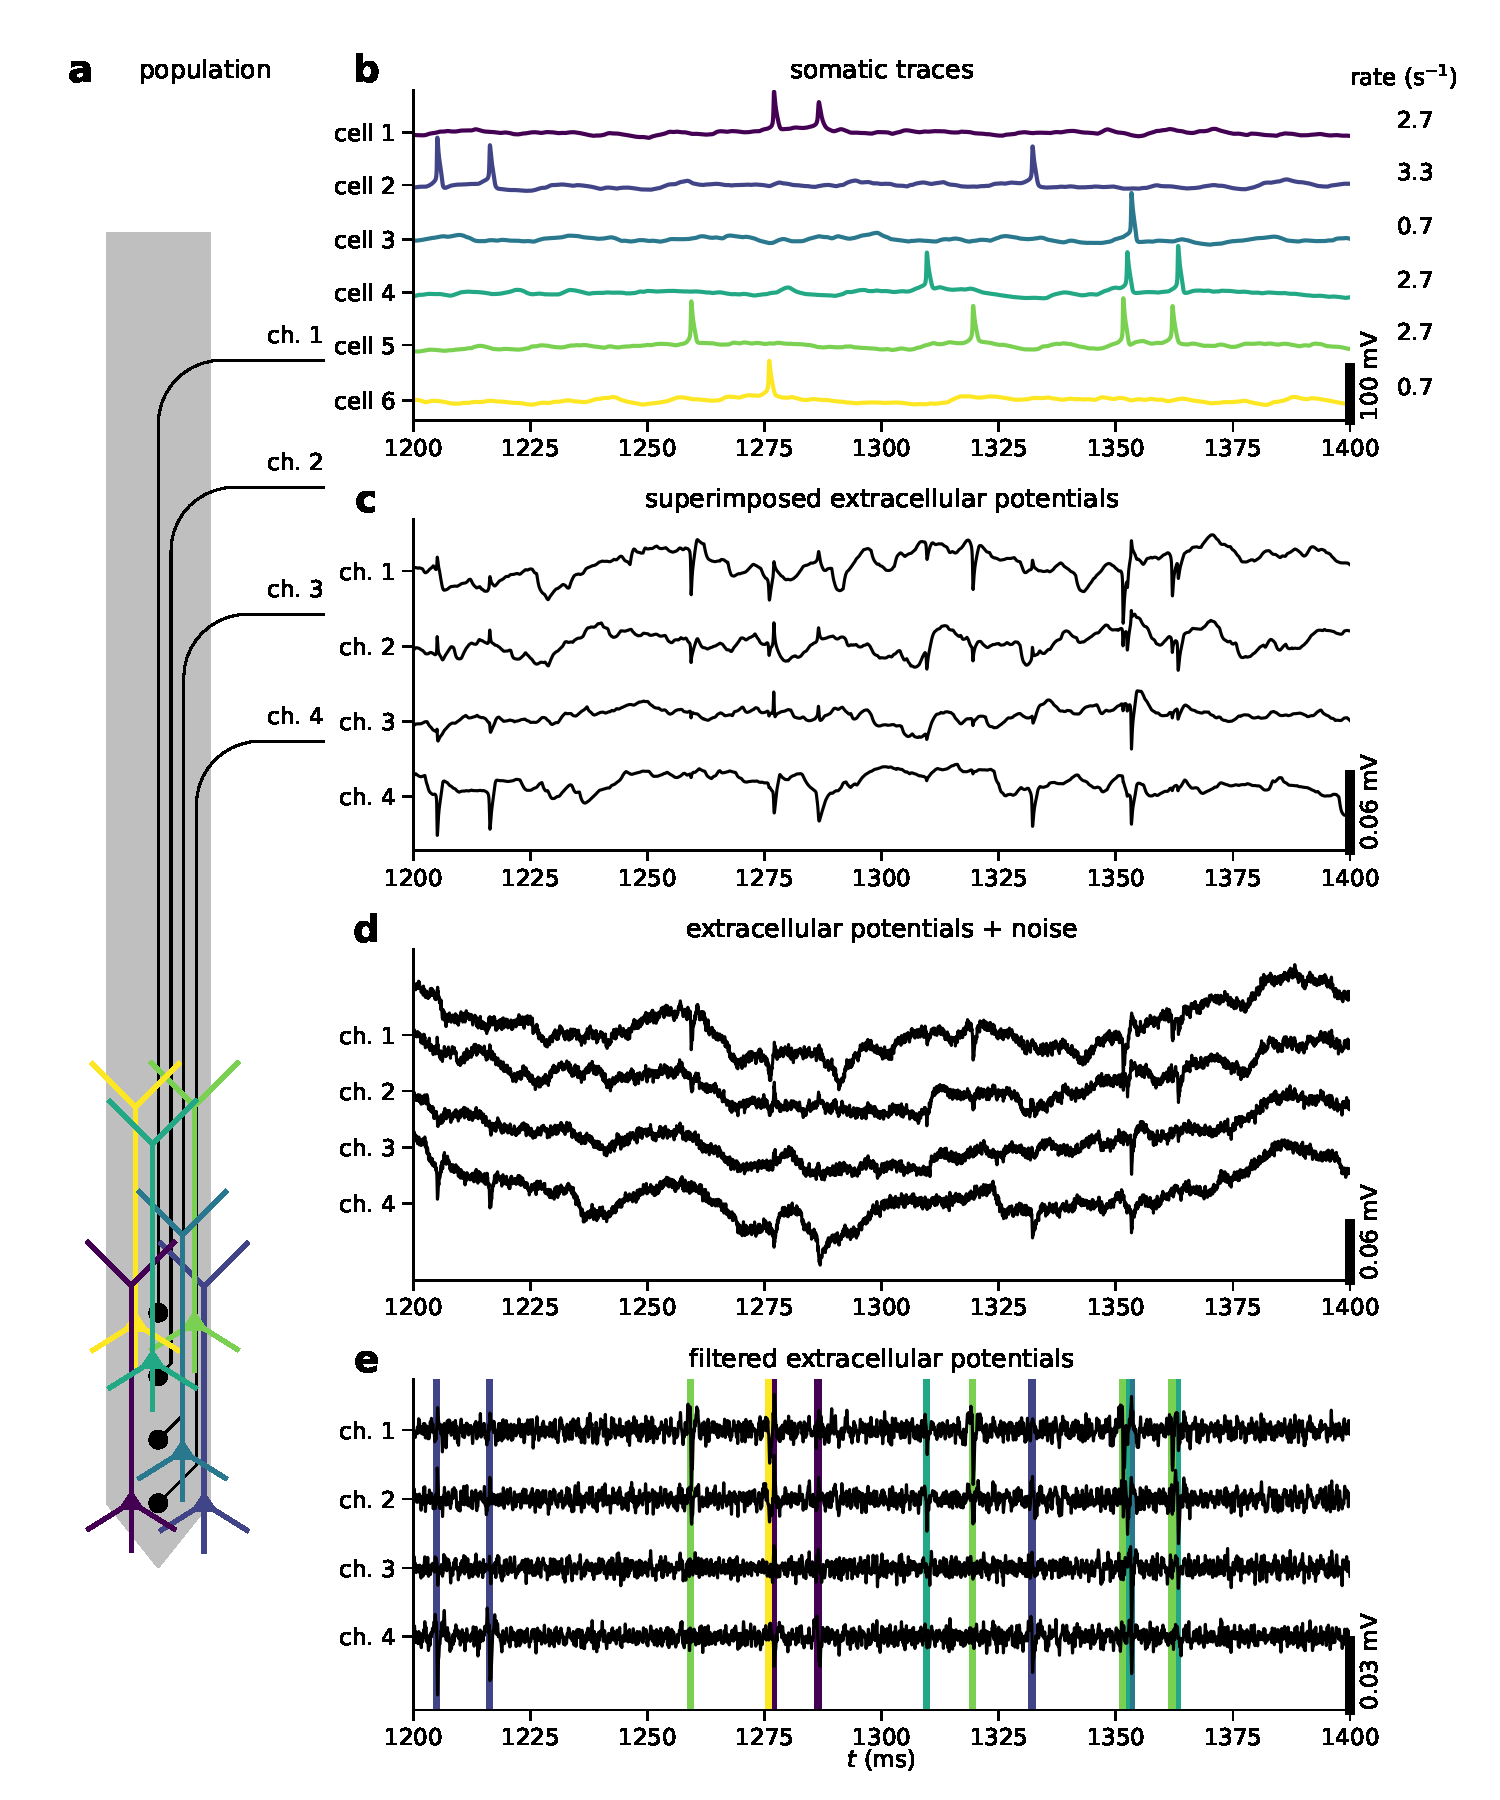
\includegraphics[width=0.8\textwidth]{Figures/Spikes/MUA-11_vII}
\end{center}
\caption[]{\textbf{MUA tetrode}
\ehtxt{based on} Hagen (2015):
Example benchmarking data for in vivo tetrode recordings. 
\ehtxt{(a) Illustration of tetrode geometry with its four contacts surrounded by six cortical pyramidal neuron models. 
(b) Somatic voltages used to assess ground-truth spike times.}
(c) Extracellular potential generated by population of six cortical pyramidal neurons.  
(d) Raw benchmarking data found from superposition of population potentials (from panel c) and synthesized model noise. 
(e) Filtered benchmarking data (corresponding to signals in (d)) showing MUA". 
\ehtxt{Colored, vertical lines denote ground-truth spike times of individual cells.} 
Adapted from \citeasnoun**{Hagen2015}.
}
\gen{Vi maa faa markert ground-truth spike times i figuren paa et vis.}
\gen{Kan vi kan legge til et panel som illustrerer en tetrode?}
\ehnote{Bra naa? Noen fontsizes maa oekes bare. Er soma potensial nok for aa si noe om ground truth?}
\ghnote{Ville kanskje bli lettere aa finne igjen spikes om vi bare viser f.eks. 100 ms av simuleringen?}
\label{fig:Spikes:MUA-tetrode}
\end{figure}
%%%


\subsection{\blue{Spike extraction and sorting}}  
With only a single recording contact, the most direct way to analyse the MUA is to simply detect and count the spikes in the recorded signal trace. Here a suitable detection procedure must be used. This typically involves thresholding where only voltage deflections larger than a preset threshold depending on the ambient noise level, are counted as spikes.
\gen{Kanskje vi kunne laget en enkel figur her som illustrerte spike detection her (kanskje inspirert av noen av panelene i Figur 1 i Einevoll2020? Jeg synes ikke vi trenger aa gaa inn paa prisnipper for spike sorting siden dette vel er mer "dataanalyse" enn vi ellers har planlagt aa ha med i boka.
}

Today, spikes are typically recorded with multielectrodes, for example, tetrodes with four closely positioned recording contacts (\Fref{fig:Spikes:MUA-tetrode}), linear multielectrodes (polytrodes) with tens of contacts positioned along a straight line, or spade-like multielectrodes with many hundred tiny contacts arranged in rectangular patterns on an electrode shaft \cite**{Jun2017}.  On these multielectrodes, the same spike will in general show up on several contacts, and a process known as \emph{spike sorting}~\cite**{Quiroga2007} is required to (i) properly count spikes and (ii) to sort recorded spikes into contributions from individual neurons as is often the goal. 

To develop and validate methods for spike sorting, benchmarking data where the `ground truth' is known is highly desirable. Experimental benchmarking data is hard to come by as they require simultaneous recording of intracellular action potentials and corresponding extracellular spikes. However, model-based benchmarking data is an attractive alternative~\cite**{Einevoll2012} and the generation of such data has been pursued in several projects
\cite**{CamunasMesa2013,Hagen2015,MondragonGonzalez2017,Buccino2020}. 

An example is given in \Fref{fig:Spikes:MUA-tetrode} where virtual MUA signals recorded by a tetrode are simulated  \cite**{Hagen2015}. In the simulation, six cortical neurons were placed around a tetrode, and driven to action-potential firing by a combination of excitatory and inhibitory synaptic inputs. The true firing times of the neurons are shown in Panel B, which shows their somatic membrane potential dynamics. The raw extracellular signals are shown in Panel C \gex{where} the simultaneous extracellular signatures of this firing can be seen as sharp negative peaks in some or all of the four channels. To mimic the situation seen in experiments, noise with the same statistical properties as what is seen in real tetrode experiments, is added to the signal in panel D. Panel E shows high-pass filtered signals, that is, the MUA signals to be used as benchmarking data for testing spike-sorting algorithms.

\ghnote{Action potentials om hva nevroner gjoer (Vm) og spikes om hva man ser utenfor. I traad med det vil det kanskje bli feil aa si true spike-times? Nevroner spiker ikke. De fyrer aksjonspotensialer....}
%The final MUA data clearly shows how an action potential from a single neuron is seen
%simultaneously as spikes on several of the tetrode contacts. 


%%%%
%\begin{figure}[!ht]
%\begin{center}
%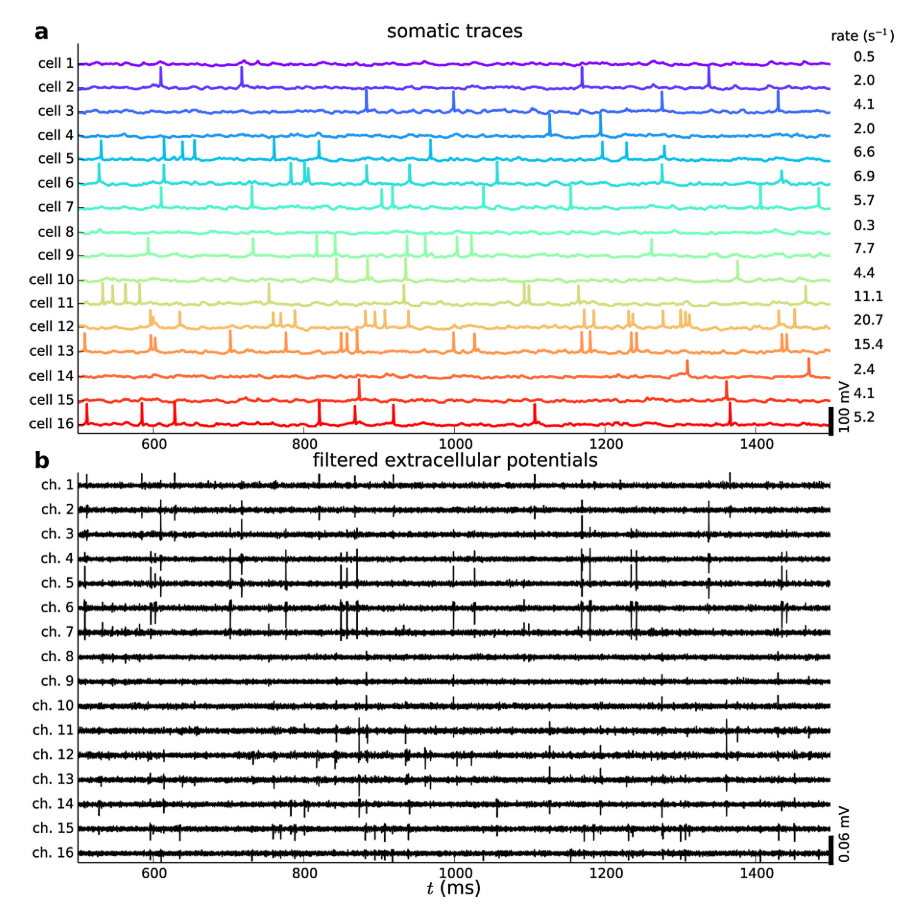
\includegraphics[width=0.8\textwidth]{Figures/Spikes/MUA-10}
%\end{center}
%\caption[]{\textbf{MUA linear multielectrode (polytrode)}
%Fra Hagen 2015: Excerpts of intracellular and extracellular recordings for the 16 cells included in the example 16-channel polytrode benchmarking data set. 
%(a) Somatic membrane potentials. Firing rates of cells 1-16 averaged over the 120 s real-time duration of the simulation are listed on the right hand side. (b) Superposition of extracellular potentials from all neurons and model noise, after band-pass filtering."
%}
%\gen{Kan vi kan legge til et panel som illustrerer polytroden?}
%\label{fig:Spikes:MUA-polytrode}
%\end{figure}
%%%%

\subsection{\blue{Population firing-rate estimation from MUA}}  
\gex{Whether or not a spike from a particular neuron rises above the ambient noise level and 
can be identified from an electrode recording, depends on several factors.} One is the volume density and morphological shapes of active neurons around the contact. Another is the impedance and size of the contact itself. As discussed in \Fref{sec:Spikes:electrode_size} large electrode contacts will tend to reduce the spike amplitude through a spatial averaging effect, making it difficult to identify individual spikes from the recorded signal. 
\gex{In situations where individual spikes cannot be identified}, the MUA signal can instead be used to provide useful insight into the combined firing rate of the neurons surrounding the contact ~\cite**{Schroeder1998,Schroeder2001,Ulbert2001}. To extract such information, the high-pass filtered extracellular potential recorded by the electrode is rectified, i.e., its absolute value is taken. 

The principle behind this `rectification' approach is illustrated in \Fref{fig:Spikes:MUA-rectifify}. \gex{The basic assumption, namely that the rectified MUA signal is proportional to the combined firing rate, is intuitively justified if only a single neuron contributes with spikes. Then the rectified spike signal will signal whether a spike has occurred or not. With several neurons  contributing, all producing identical spikes, the rectified MUA signal will still be expected to be proportional to the combined firing rate as long as the firing is sparse so that there is little overlap in time between the spikes of the contributing neurons. However, if there is a substantial temporal overlap between the spikes there will be cancellation effects from negative `sodium signals' in one spike overlapping the positive `potassium signal' in another spike. The rectified summed signal will then become smaller than the sum of the individual rectified spikes, resulting in an underestimated firing rate.

Another possible complication is that the contributions from the various spiking neurons around the recording contact will vary in size. However, if the contributing neurons belong to the same neuronal population and have statistically the same firing behaviour, the rectified MUA should still reflect the population firing rate. 
}


%%%
\begin{figure}[!ht]
\begin{center}
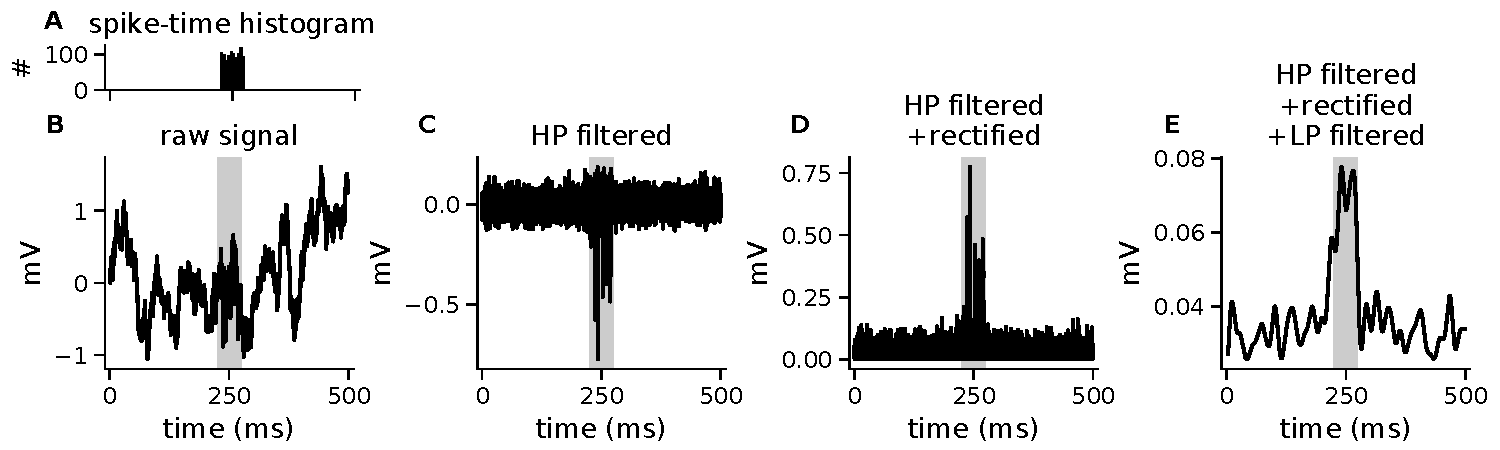
\includegraphics[width=1.\textwidth]{Figures/Spikes/fig_hay_MUA.pdf}
\end{center}
\caption[]{{\bf Illustration of MUA rectification}
{\bf A:} Spike-time histogram of the spikes.
{\bf B:} The raw signal, containing artificially generated noise, with spikes superimposed on the signal 
according to the spike-times from {\bf A}. For each spike time the spike shape is randomly chosen from the grid in \fref{fig:Spikes:MultiCompartment}{\bf A}.
{\bf C:} High-pass filtered (>300~\si{\hertz}) version of the raw-signal in {\bf B}.
{\bf D:} Rectified version (that is, the absolute value is taken) of high-pass filtered signal in {\bf C}.
{\bf E:} Low-pass filtered (<50~\si{\hertz} version of signal in {\bf D}.
\gen{Figure illustrating principle behind MUA from rectification method}
\gen{Can you make such a figure, Torbj{\o}rn?}\tvnnote{OK?}
 \ghnote{Forstaar ikke helt hva som skjer. A: Hva betyr inserted? Bedre med pre-set spike histogram? B: Bedre med constructed raw signal? Spike time: Hver soeyle i histogramet har en bredde. Hvor ble spiken satt innenfor dette intervallet? Dette ble noe kondensert, og kanskje vi boer skrive mer omfiguren i broedteksten?}
}
\label{fig:Spikes:MUA-rectifify}
\end{figure}
%%%

This rectification approach was used to estimate firing rates of cortical populations of neuron in the rat barrel (somatosensory) cortex based on multielectrode laminar recordings~\cite**{Einevoll2007,Blomquist2009}. To test the validity of the method, a modeling study was pursued where an analogous virtual (in silico) experiment was performed~\cite**{Pettersen2008}. Specifically, about thousand layer-5 cortical pyramidal neurons with somas arranged in a cylindrical disc, mimicking a neuronal population in rat barrel cortex, was considered (\Fref{fig:Spikes:MUA-population}). 
\gex{The neurons received synaptic inputs resembling those seen experimentally following whisker flicks}. Extracellular potentials were computed for a set of contact positions along the central axis of the cylinder (\Fref{fig:Spikes:MUA-population}B).

%%%
\begin{figure}[!ht]
\begin{center}
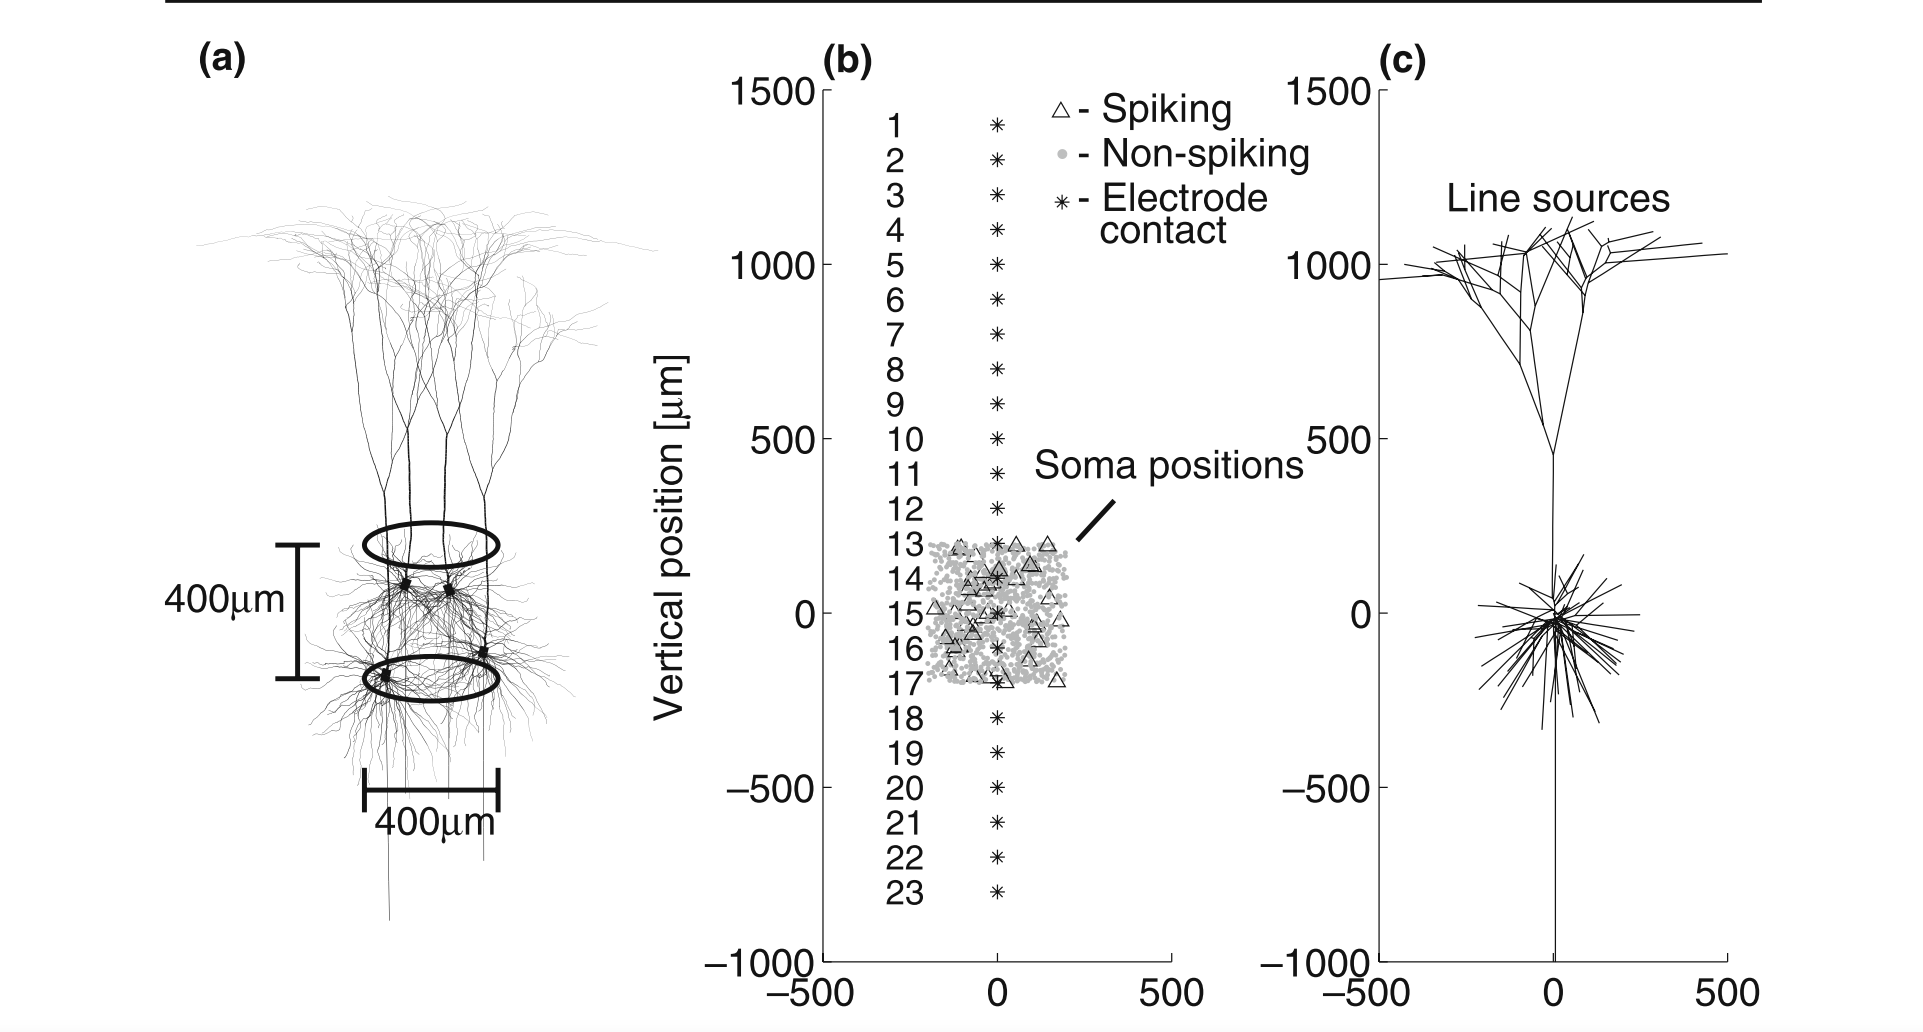
\includegraphics[width=0.8\textwidth]{Figures/Spikes/MUA-2}
\end{center}
\caption[]{
From Pettersen 2008a: \textbf{Schematic illustration of neural population created from pyramidal layer-5 neuron templates.} (b) Somas of neuronal templates are placed randomly inside a cylindrical annulus with height h=0.4 mm, outer diameter d=0.4 mm, and inner diameter 0.1 mm. One thousand cells are non-spiking (dots), while 40 cells produce a single spike following synaptic stimulation (triangles). The electrode point contacts (stars) are aligned on the central axis of the cylindrical annulus. (c) Illustration of line-source method where the transmembrane currents passing through the 
segments of the displayed branches are modeled as line segments with uniform current density.}
\label{fig:Spikes:MUA-population}
\end{figure}
%%%

An example result is shown in \Fref{fig:Spikes:MUA-ApicalSynapses}. Here panel A shows the total extracellular potential following the synaptic activation of the population. The signal is dominated by the low-frequency response to the synaptic input, that is, the local-field potential (LFP). The spatial pattern of the signal across recording channels reflects the
spatial distribution of synaptic inputs onto the pyramidal neurons. In this example, excitatory synapses are placed on the apical dendrites while inhibitory synapses are placed on the basal dendrites. \ghnote{Kan de to figurene som viser dette eksempelet slaaes sammen? Trengs panel C i den foerste?} \gen{Denne kommentaren er kanskje ikke lenger aktuell?}
%The dominance of low frequencies in the signal is illustrated in panel B showing the Fourier transformed signal, that is, the amplitude of each frequency component, for three of the channels. Here it can be seen that the frequencies up to 100 Hz dominate the signal completely, that is, have the highest amplitudes (and power, corresponding to the amplitude squared) \ghnote{Er det noe med at power er disse koeffesientene delt paa roten av 2? Har aa gjoere med at man faar bidrag fra pluss og minus-amplituder etc. Christine, masterstudent, styrte litt med dette, og det er visst noen bugs i en PSD-utregning Torbjorn sendte oss. Maa finne ut av dette.}. 

%%%
\begin{figure}[!ht]
\begin{center}
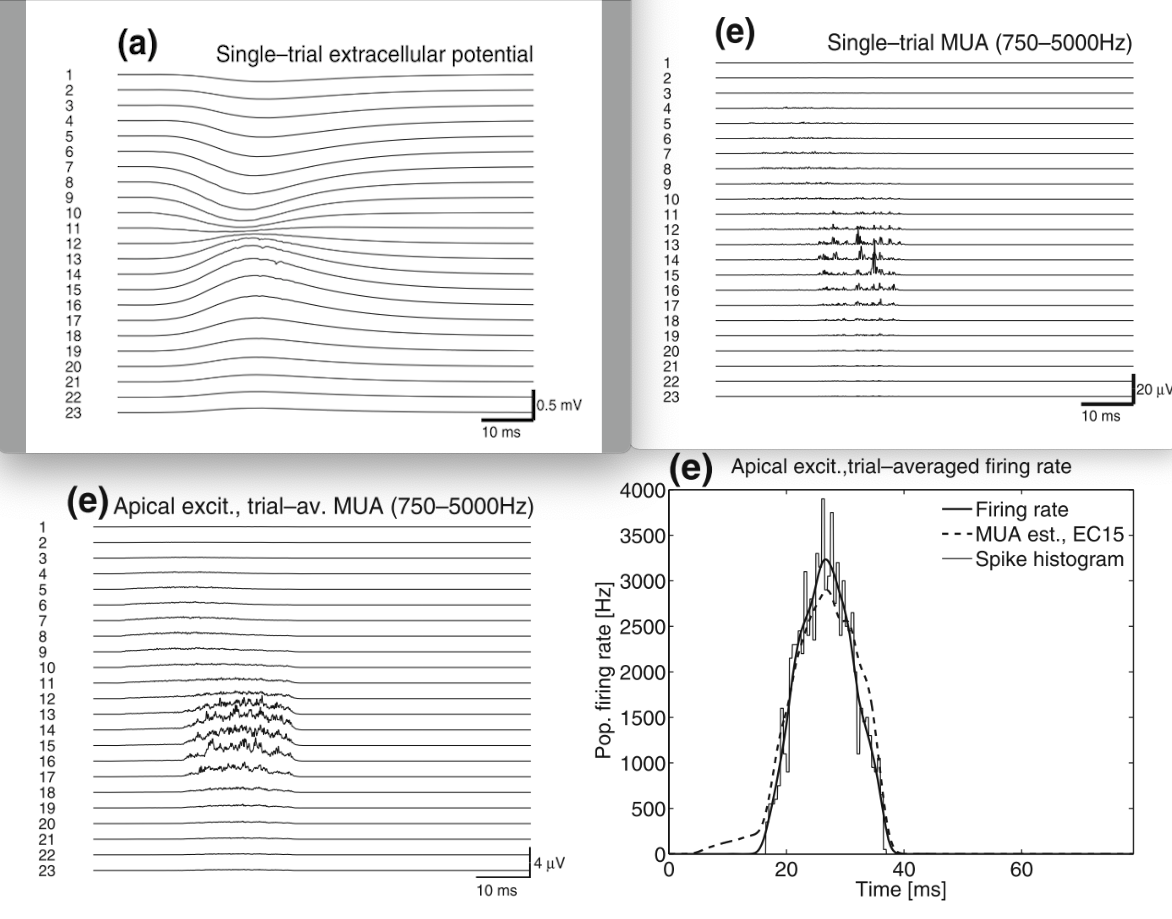
\includegraphics[width=0.8\textwidth]{Figures/Spikes/Spikes-MUA-barrel} 
%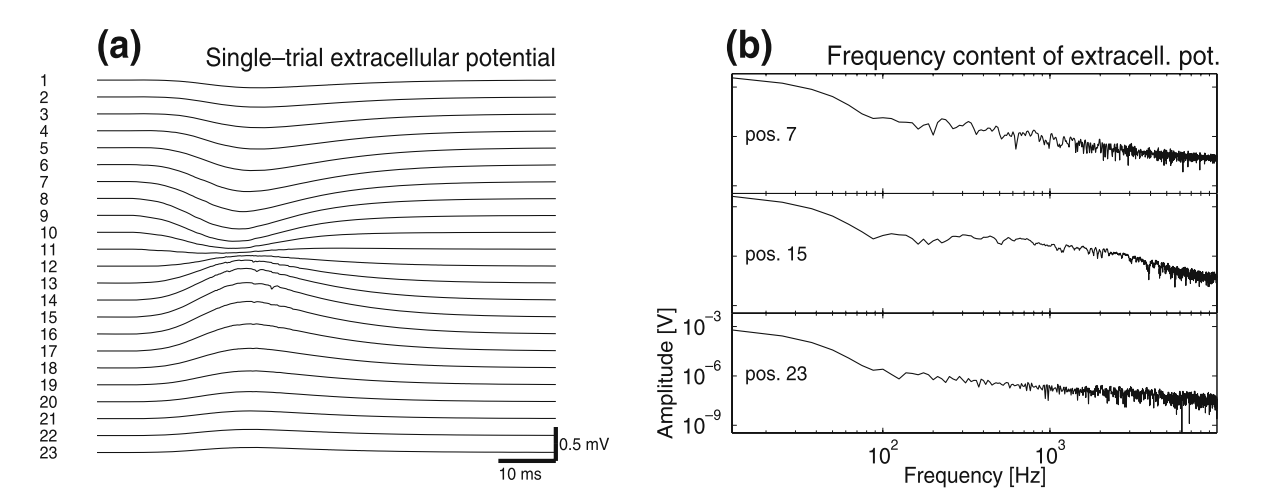
\includegraphics[width=0.8\textwidth]{Figures/Spikes/MUA-3} \\
%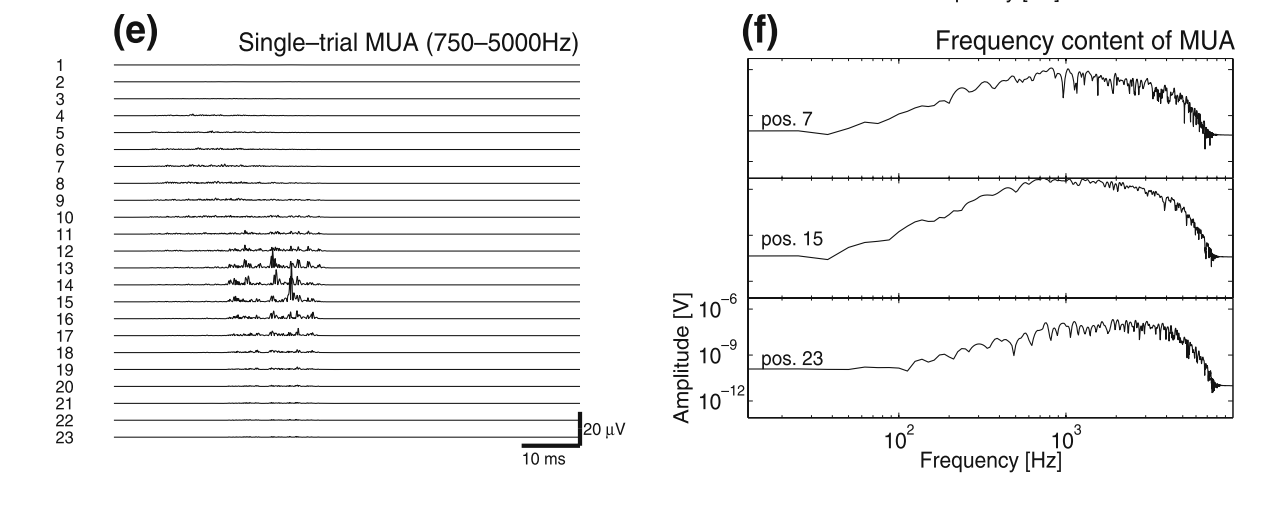
\includegraphics[width=0.8\textwidth]{Figures/Spikes/MUA-4} \\
%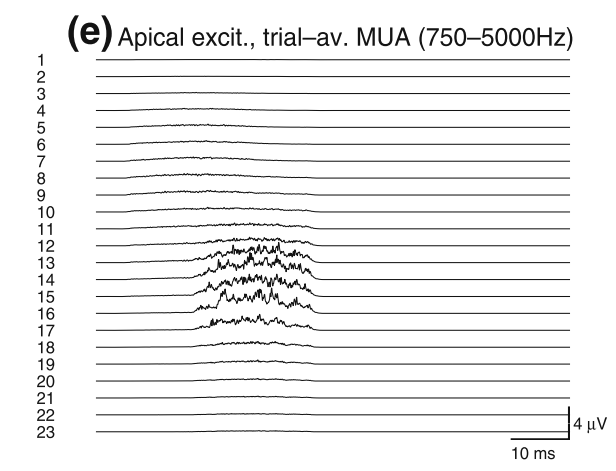
\includegraphics[width=0.4\textwidth]{Figures/Spikes/MUA-5} 
%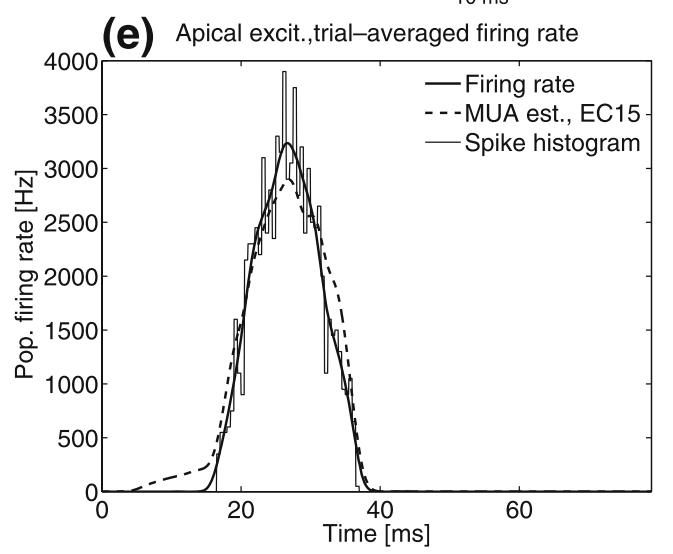
\includegraphics[width=0.4\textwidth]{Figures/Spikes/MUA-7} 
\end{center}
\caption[]{
From Pettersen 2008a: \textbf{Extracellular potentials at electrode contacts 1-- 23 for apically stimulated population.} 
\gex{
(A) Single-trial raw (unfiltered) extracellular potentials. 
%(b) Frequency content, i.e., Fourier amplitudes, of raw potentials in (a). 
(B): "(e)" MUA, i.e., high-pass filtered (750 -- 5.000 Hz) and rectified content of potentials in (a). 
%Middle right "(f)" Frequency content of the MUA in (e) prior to rectification. 
The mean synaptic onset times are stochastically distributed around 20 ms with a standard deviation of $\sigma$=5 ms.
(C) "(e)": MUA, i.e., high-pass filtered (750 -- 5.000 Hz), rectified and then trial-averaged signals for apically excited population. 
(D)} "(e)": Spike \ghnote{Spike eller AP? Er det pirkete aa henge seg opp i dette?} histogram (bin width 0.5 ms), `true' population firing rate and estimated firing rate from the MUA of electrode contact 15. The amplitude of the estimated firing rate has been fitted to minimize the relative mean square deviation er  between the estimated and `true' population firing rates. 
\gen{Refer to Pettersen2008 for detailed explanation.}  \ghnote{Boer vi definere population firing rate, eller er det selvforklarende?},
}
\label{fig:Spikes:MUA-ApicalSynapses}
\end{figure}
%%%

While the spikes are buried by the low-frequency components in the raw signal, they can be extracted by high-pass filtering 
and subsequent rectification. \gex{Results are shown in \Fref{fig:Spikes:MUA-ApicalSynapses}B.} 
A first observation is that the remaining signal is confined to channels deep in the cortex, that is, close to the somas of the neurons in the populations.This reflects that extracellular signatures of action potentials are typically confined to within 100~$\mu$m from the soma, cf. \Fref{fig:Spikes:DifferentNeuronModels}. A second observation is that the MUA signals only last for about 20~ms, which turns out to be the time period in which the neurons in the model fire action potentials~\cite**{Pettersen2008}. A third observation is that the MUA signal is not smooth, but `noisy' in the sense that it consists of a collections of sharp peaks of different heights. This `noisiness' stems from the inherent randomness both in the times of spiking and the positions of the somas of the low number (40) of spiking neurons in the population. 

In sensory systems it has been common to measure trial-averaged responses, that is, the response averaged over many repetitions of the same stimulus. The rationale is that this procedure highlights the contributions from sensory input in that the effects of other synaptic inputs and noise in sensory neurons are reduced. The trial-averaged MUA found from averaging MUA results from forty model trials, is shown in panel C of \Fref{fig:Spikes:MUA-population}, revealing a much less `noisy' signal. 

The obvious next question is to what extent the resulting MUA signal gives a good measure of the population firing rate. Unlike in experiments, the true underlying firing rate is known in the model, allowing for a quantitative comparison. The question was studied in detail for the model in question in \citeasnoun**{Pettersen2008}. The noisyness of MUA signals from individual trials (\Fref{fig:Spikes:MUA-population}B) did not allow for accurate estimation of firing rates in individual trials. However, accurate estimates for trial-averaged firing rates (commonly referred to as Post Stimulus Time Historgrams (PSTHs)) could be obtained from trial-averaged MUA signals. An example is given in \Fref{fig:Spikes:MUA-ApicalSynapses}D. Here a firing-rate estimate based on the MUA signal from one of the recording channels positioned at a depth in the midst of somas of the population is compared with the true, temporally smoothed firing rate. The overall agreement is observed to be quite good.

One deviation between the real and predicted firing rate is that the \gex{MUA-based analysis} predicts a non-zero firing rate prior to the onset of true firing, the reason being that the synaptic input current itself gives a contribution to the MUA signal. Another deviation is that the \gex{MUA analysis} predicts a too low maximum firing rate, due to cancellations of signal contributions from temporally overlapping spikes from different neurons. This latter effect increases with increasing firing rates and can be remedied by assuming a supralinear relationship between the MUA signal and firing rate \cite**{Pettersen2008}.  The accuracy of the population firing rate can also be improved by using MUA signals from several adjacent recording channels in the estimation \cite**{Pettersen2008}.  
 
The accuracy of this MUA-based estimation of population firing rates will depend on the specific situation considered. In \citeasnoun**{Pettersen2008}, it was, for example, found that the prediction was slightly more accurate when the population in \Fref{fig:Spikes:MUA-population} is driven by excitatory inputs onto the basal dendrites rather than onto the
apical dendrites as in \Fref{fig:Spikes:MUA-ApicalSynapses}.

 
%
%%%%
%\begin{figure}[!ht]
%\begin{center}
%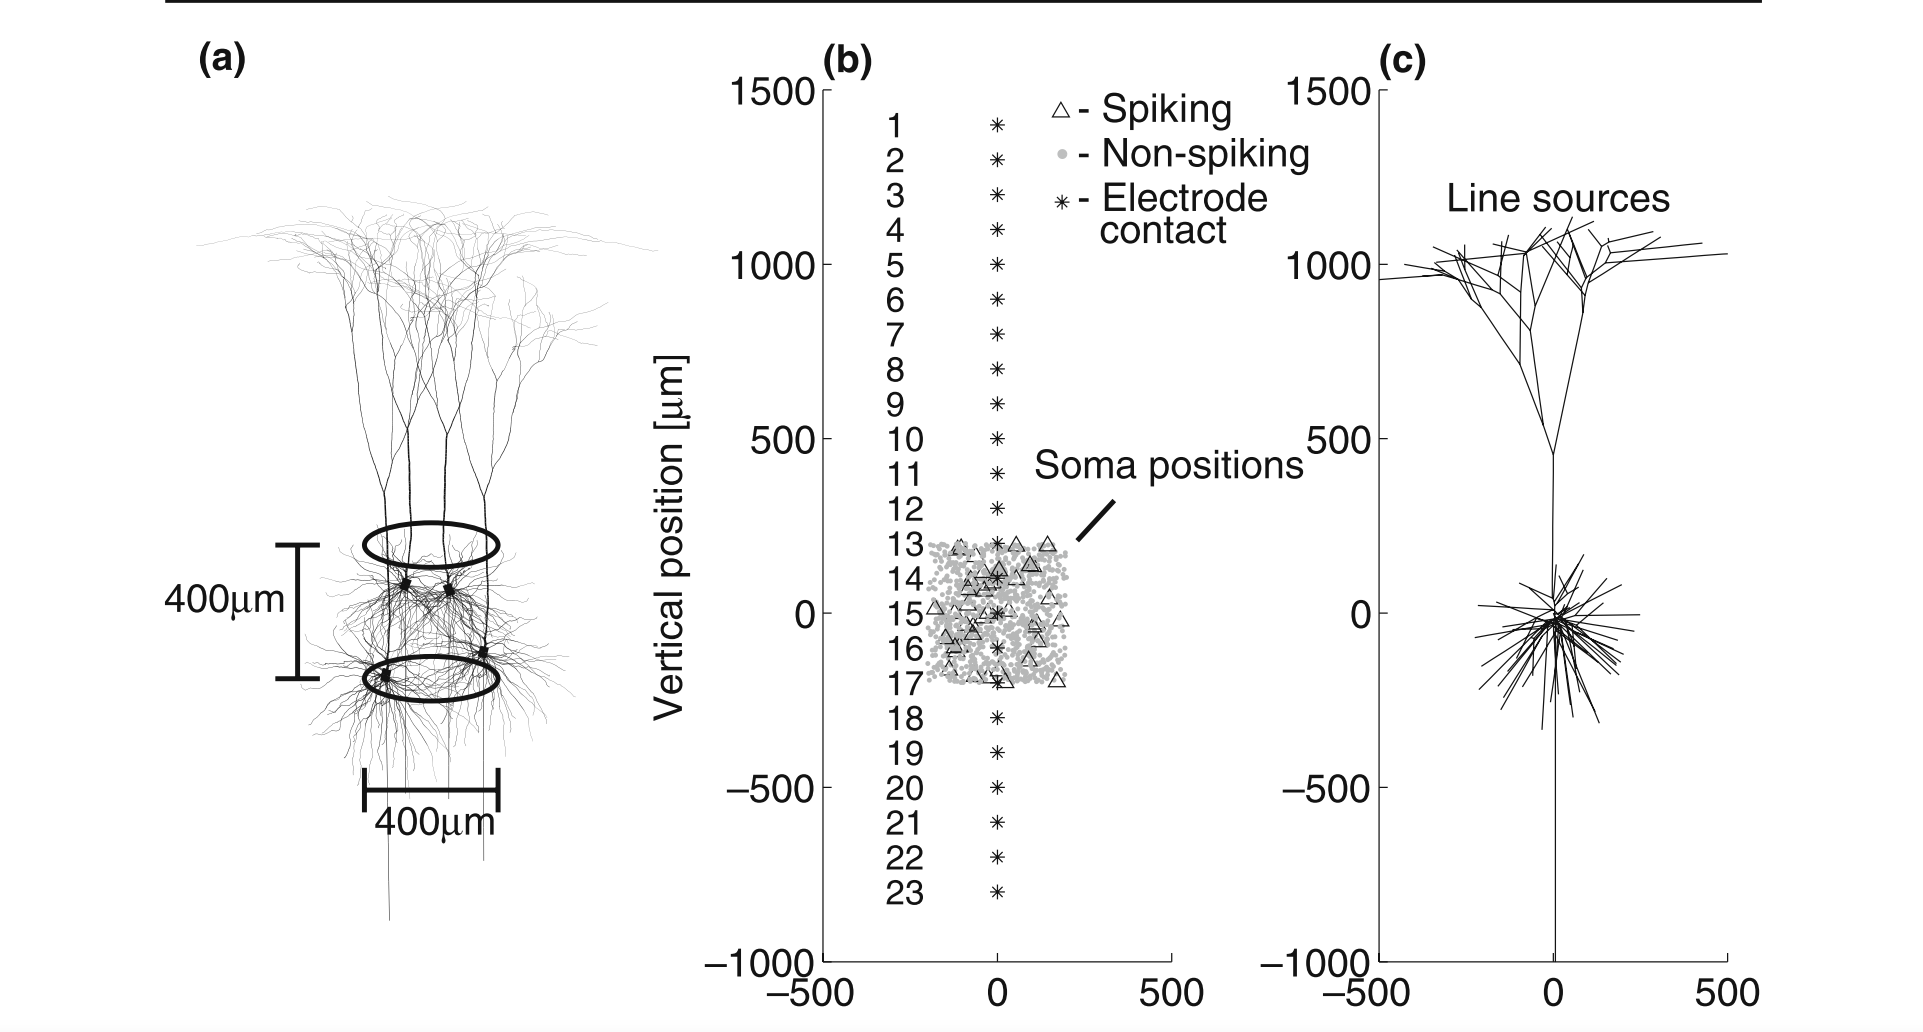
\includegraphics[width=0.8\textwidth]{Figures/Spikes/MUA-2}
%\end{center}
%\caption[]{\textbf{MUA}}
%\label{fig:Spikes:MUA-A}
%\end{figure}
%%%%
%

%
%%%%
%\begin{figure}[!ht]
%\begin{center}
%\includegraphics[width=0.4\textwidth]{Figures/Spikes/MUA-6}\\
%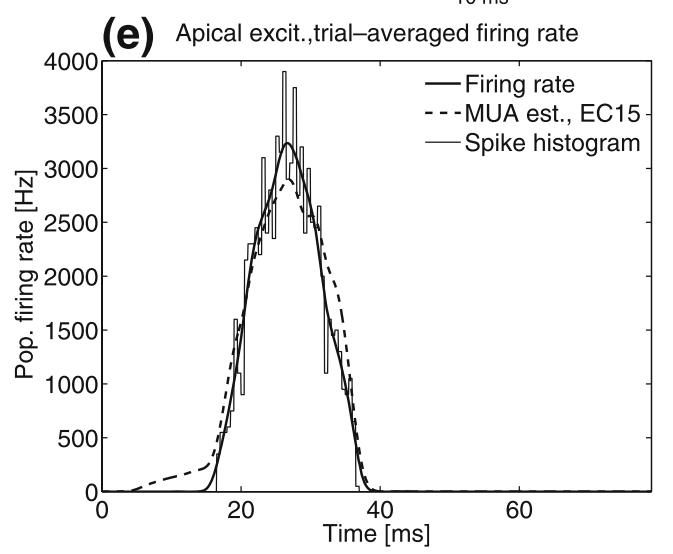
\includegraphics[width=0.4\textwidth]{Figures/Spikes/MUA-7}
%\end{center}
%\caption[]{\textbf{MUA}}
%\label{fig:Spikes:MUA-C}
%\end{figure}
%%%%
%
%%%%
%\begin{figure}[!ht]
%\begin{center}
%\includegraphics[width=0.8\textwidth]{Figures/Spikes/MUA-8}
%\end{center}
%\caption[]{\textbf{MUA}}
%\label{fig:Spikes:MUA-D}
%\end{figure}
%%%%
%

%\section{\red{Insights from MUA studies}} 
%\ghnote{I added this kind of subsection to most of the Part 2 - sections. I thought it might be an idea to finish the MUA, LFP, ECoG and EEG sections with summaries of what these modalities typically tell us, i.e. in terms of (i) what aspects of neural activity they reflect (spikes, synaptic inputs, dendritic ion channels, which ion channels, which kind of neurons, something on network structure, cell orientation, cortical folding etc.), and what what they can tell us about cognitive states (attentive, drowsy etc.). I am not sure about this idea, though. Maybe it will be too challenging to get an overview over the literature - we dont want to put the entire Nunez-book into the EEG-chapter.}

%%%%%%%%%%%
%% Box: Spike sorting
%%%%%%%%%%%
%%\begin{boxfloat}{Spike sorting}
%%  \label{mm:box:spike-sorting}
%\subsection{\red{Box: Spike-sorting}}
%\gen{This was a Box in the Sterratt chapter}
%%
%\centerline{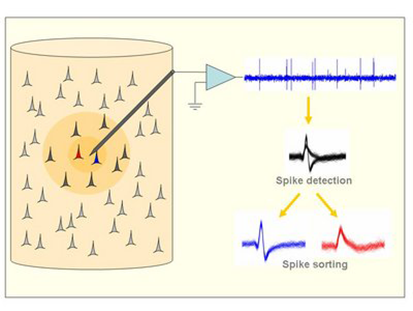
\includegraphics{Figures/Spikes/Spikes-sorting-w35-r300}}\vspace*{6pt}
%%
%A sharp electrode placed in brain tissue will pick up spiking signals from several neurons. 
%However, the shapes of the spikes will be different for the different neurons, and this can be used to sort the spikes according to their neurons of origin. This is referred to as \index{spike sorting}, 
%and is a problem of great practical importance both for neuroscience research and development of neuroprosthetic devices. 
%
%In the present day with electrodes with hundreds or thousands of electrode recording contacts, fast and accurate automatic spike-sporting methods are needed to replace time-consuming manual spike-sorting methods~\cite**{Quiroga2007}. To develop and test such automatic methods, one needs
%benchmarking spiking data where the `ground truth', that is, the actual spiking times for the contributing neurons, is known~\cite**{Einevoll2012}.
%One use of the EP modelling scheme for spikes has been to generate such benchmarking data~\cite**{CamunasMesa2013,Hagen2015,MondragonGonzalez2017}. 
%
%Modern electrodes have numerous recording contacts, often placed only some micrometers apart. Thus a spike can be measured at several contacts
%simultaneously, each contact recording a slightly different shape reflecting the different positions of the contacts relative to the spiking neuron. 
%This not only allows for accurate spike sorting, but also for estimation of the spatial position of the neuron. Likewise, the spatial variation of the 
%spike shape around the neuronal soma (see \Fref{fig:Spikes:MultiCompartment}) 
%depends on the details of the intracellular action potential and dendritic morphology thus also allowing for the 
%identification of neuron type~\cite**{Buccino2018}.    
%\gen{Figure to be adapted from Quiroga (2007).}
%%\end{boxfloat}
%%%%



%While the formulae above were derived for a neuron model with a single passive dendritic stick, similar expressions can be derived for 
%more complicated neuron models where several passive sticks protrude from the soma, see \citeasnoun**{Pettersen2008}.
%The main conclusions above hold also for these neuron models, in particular that spike widths always increase with distance and that
%the amplitude of a spike is proportional to $d^{k}$ where $k\sim1.5-2$. For neurons with many dendrites attached to the 
%soma, the contributions to the spike amplitude roughly adds up. A simple rule of thumb is that a neuron's spike amplitude is 
%roughly proportional to the sum of the cross-sectional areas for all dendrite branches attached directly onto to the soma. Neurons with many thick
%dendritic branches attached to the soma will thus generate the largest spikes. See~\citeasnoun**{Pettersen2008} for further discussion.
%
%
%{\bf TEXT COPIED FROM STERRATT CHAPTER ON 2020-10-13}
%
%\section{Dependence of spike size and shape on neuronal properties}
%
%Extracellular measurement of spikes from a neuron in living brains is blind in the sense that it is
%not known what type of neuron is recorded from when an electrode is lowered into the brain.
%Some neuron types produce spikes with larger amplitudes and/or broader shapes than
%others,
%%
%%\todo{TVN: Nevne at det ofte sorteres i "putative excitatory" og "putative inhibitory"?}
%%
%and as seen in \Fref{mm:fig:EP-spike-MultiCompartment} both the shape and amplitude 
%depend critically on recording positions. Large spike amplitudes imply that they will be more dominant in electrical recordings,
%and ideally this bias should  be considered in the analysis of joint recordings 
%of spikes from many neurons. 
%
%To understand the link between the morphology of neurons and their spike amplitudes and shapes
%it is convenient to consider ball-and-stick neurons where a passive dendrite cable `stick' is connected to a point-like soma.
%Despite its simplicity, the ball-and-stick neuron model exhibits the key qualitative features observed in
%\Fref{mm:fig:EP-spike-MultiCompartment} when the multi-compartmental EP formula in 
%\Fref{mm:equation:Ve-multi-compartment}
%is used; that is, rapid attenuation of spike amplitude and increased spike width as the distance from the soma 
%increases \cite**{Pettersen2008,Pettersen2012}. 
%
%\citeasnoun**{Pettersen2008} took advantage of the mathematical tractability of the ball-and-stick model to
%derive analytical expressions for how the amplitude of the recorded spike depends on distance from the neuron as well
%as the electric properties of the neuron. The action potentials were decomposed into contributions from
%many frequency components and each frequency component was considered individually.
%This is illustrated in \Fref{mm:fig:EP-spike-ball-and-stick-frequency} where the amplitudes of the different frequency components needed to
%represent the intracellular action potential (membrane potential) and extracellular spike respectively are shown.
%A key observation here is that for the extracellular spike, the largest contributions comes from frequencies larger than 100~hertz.
%%%%%%%%%%%
%% Figure: Action potential and its frequency content
%%%%%%%%%%%
%%\begin{cnfigure}{Figures/fig-not-pushed-to-github}
%%\begin{cnfigure}{Figures/mm/EP-spike-ball-and-stick-frequency-w90-r150}
%%\caption[]{
%%Frequency content of example intracellular (a) and extracellular spike (b).
%%%
%%%(a) Action potential used in simulations in \Fref{mm:fig:EP-spike-ball-and-stick-results}(inset) 
%%%\todo{Comment from DCS not understood.}
%%%and its frequency content. 
%%%%The intracellular spike width is defined as the
%%%%width of the AP at half amplitude and is 0.55~ms for the standard
%%%%AP, and half the value for the narrow AP. 
%%%(b) Frequency content of example extracellular spike.
%%%Inset: Typical spike shape computed a distance $r=10~\mu$m
%%%perpendicular to the dendrite at the level of soma for a ball-and-stick 
%%%neuron with diameter $d=2~\mu$m and infinite dendrite length.
%%%Here the intracellular action potential in left panel was imposed as a voltage-clamp in the soma.
%%%The extracellular spike width is defined as the width of the negative phase at 25\% of its maximum
%%%amplitude and is 0.44~ms for the example spike.
%%%The amplitude (peak-to-peak value) of the spike is $56~\mu$V  
%%\todo{Figure + caption to be updated. Will only include standard AP in final figure.} 
%%Adapted from \citeasnoun**{Pettersen2008}.
%%}
%%\label{mm:fig:EP-spike-ball-and-stick-frequency}
%%\figpermOurs
%%\end{cnfigure}
%
%
%%\todo{Explain the idea that the question is about how currents entering the soma during the AP returns through the dendrite}
%
%\citeasnoun**{Pettersen2008} derived simple formulae relating the intracellular action potential to the extracellular spike for two limiting cases:
%when the recording is done near to the soma or far away from the soma. For recordings near the soma the 
%amplitude $|\hat{V}_\mathrm{e,near}(f,\vec{r})|$ of the spike signal for each frequency component with frequency $f$ was found to be approximated
%by
%%
%\begin{equation}
%  |\hat{V}_\mathrm{e,near}(f,\vec{r})| 
%  \propto \frac{d^{3/2}}{r} \sqrt{ \frac{f c_\mathrm{m}}{r_\mathrm{a}} }  |\hat{V}_\mathrm{s}(f)| 
%  \label{mm:equation:Ve_near}
%\end{equation}
%%
%Here $|\hat{V}_\mathrm{s}(f)|$ is the amplitude of frequency component of the soma membrane potential at the same
%frequency (see \Fref{mm:fig:EP-spike-ball-and-stick-frequency}).
%For recording positions far away from the soma, the following expression was instead found:
%%%%
%\begin{equation}
%  |\hat{V}_\mathrm{e,far}(f,\vec{r})|  \propto d^{2} \frac{|\cos \theta| }{r^2  r_\mathrm{a}}  |\hat{V}_\mathrm{s}(f)| 
%  \label{mm:equation:Ve_far}
%\end{equation}
%%%%
%In these formulas, $d$ is the diameter of the dendritic
%stick, $c_\mathrm{m}$ the specific membrane capacitance, and $r_\mathrm{a}$ the specific axial resistance.  
%

%%%%%%%%%%%
%% Figure: Spike widths and amplitudes
%%%%%%%%%%%
%\begin{cnfigure}{Figures/mm/EP-spike-ball-and-stick-results-w100-r150}
%\caption[]{
%Spike widths (left) and (peak-to-peak) spike amplitudes (right) as a function of
%distance from soma for a detailed pyramidal cell model (pyramidal) and two
%types of ball-and-stick models: long, finite ball-and-stick
%model (fin.~stick, long) with diameter $d=2~\mu$m and length
%$l=1$~mm and a short, finite ball-and-stick model (fin.~stick, short) with diameter $d=1~\mu$m and length $l=0.2$~mm,
%see \Fref{mm:fig:EP-spike-ball-and-stick-neuron-models}.
%The intracellular action potential shown in the inset in the left panel of 
%\Fref{mm:fig:EP-spike-ball-and-stick-frequency} was imposed as a voltage-clamp in the soma.
%The EP was recorded in the
%somatic plane normal to the stick/primary apical dendrite. 
%In right panels guidelines illustrating the power-law decays $1/r$ and
%$1/r^{2}$ have been added. 
%For further details see \citeasnoun[Figure 6]{Pettersen2008}.
%\todo{Figure + caption to be updated. Adapted from \citeasnoun**{Pettersen2008}.}
%}
%\label{mm:fig:EP-spike-ball-and-stick-results}
%\figpermOurs
%\end{cnfigure}


%\paragraph{Spike amplitude dependence on distance}

%%%%%%%%%%%%%%%%%%%%%%%%%%%
%% Box: Spike sharpness
%%%%%%%%%%%    
%\begin{boxfloat}{Spike sharpness}
%  \label{mm:box:spike-sharpness}
%There are several qualitative insights regarding the sizes and widths of spikes that can 
%be found from the near-field and far-field formulae in Equations~\Fref{mm:equation:Ve_near} and 
%\Fref{mm:equation:Ve_far}, respectively. One relates directly to the shape of the spike:
%in the near-field expression, the high-frequency components of the spike is amplified 
%compared to the low-frequency components, that is, $\hat{V}_\mathrm{e,near}(f,r) \propto \sqrt{f}$.
%Thus close to the soma the spike is observed to be sharper than the intracellular action potential
%as observed in the insets in \Fref{mm:fig:EP-spike-ball-and-stick-frequency}. 
%In the far-field regime there is no such high-frequency amplification ($\hat{V}_\mathrm{e,near}(f,r) \propto f^0 \sim 1$).
%As a consequence, spikes measured far away from the soma will have less high-frequency content than those measured close to soma.
%Thus the far-away spikes will be blunter and have larger spike widths as seen in the spike-width panel of 
%\Fref{mm:fig:EP-spike-ball-and-stick-results}.
%%
%%\centerline{\includegraphics{Figures/mm/MEA-1-w43-r300}}\vspace*{6pt}
%%
%\end{boxfloat}
%%%%%%%%%%%%%%%%%%%%%%%%%%%%%%%%





%
%%%%%%%%%%%
%% Sidebox: Fourier sum
%%%%%%%%%%%
%\begin{sidebox}
%Time signals, such as the time course of a spike $V_\mathrm{e}(t)$,  can conveniently 
%be represented as a sum of \firstterm{Fourier components} with different frequencies $f$. 
%Such a Fourier sum can be constructed in
%various ways. The derivations in 
%Section~\Fref{mm:sec:spike-widths-amplitudes}, building on \citeasnoun**{Pettersen2008}, use the  
%convention that a time signal $S(t)$ is the real part of the complex sum $\sum_{f}  \hat{S}(f) \exp (j 2 \pi f t)$. 
%Here $j$ is the unit of imaginary numbers, and  $\hat{S}(f)$ is in general a complex number. 
%\end{sidebox}
%%
%
%%%%%%%%%%%
%% Figure: Spike widths and amplitudes
%%%%%%%%%%%
%\begin{cnfigure}{Figures/mm/EP-spike-ball-and-stick-results-w100-r150}
%\caption[]{
%Spike widths (left) and (peak-to-peak) spike amplitudes (right) as a function of
%distance from soma for a detailed pyramidal cell model (pyramidal) and two
%types of ball-and-stick models: long, finite ball-and-stick
%model (fin.~stick, long) with diameter $d=2~\mu$m and length
%$l=1$~mm and a short, finite ball-and-stick model (fin.~stick, short) with diameter $d=1~\mu$m and length $l=0.2$~mm,
%see \Fref{mm:fig:EP-spike-ball-and-stick-neuron-models}.
%The intracellular action potential shown in the inset in the left panel of 
%\Fref{mm:fig:EP-spike-ball-and-stick-frequency} was imposed as a voltage-clamp in the soma.
%The EP was recorded in the
%somatic plane normal to the stick/primary apical dendrite. 
%In right panels guidelines illustrating the power-law decays $1/r$ and
%$1/r^{2}$ have been added. 
%For further details see \citeasnoun[Figure 6]{Pettersen2008}.
%\todo{Figure + caption to be updated. Adapted from \citeasnoun**{Pettersen2008}.}
%}
%\label{mm:fig:EP-spike-ball-and-stick-results}
%\figpermOurs
%\end{cnfigure}
%
%%%%%%%%%%%
%% Figure: Frequency-dependent distribution of return currents
%%%%%%%%%%%
%\begin{cnfigure}{Figures/mm/EP-spike-ball-and-stick-sketch-w70-r300}
%%\begin{cnfigure}{Figures/fig-not-pushed-to-github}
%\caption[]{Illustration of ball-and-stick neuron and its frequency-dependent 
%distribution of dendritic return currents following injection of a sinusoidal current into the soma.
%The net current entering the soma will enter the dendrite as an axial current, and return to the 
%ECS via the dendrite membrane. The inset shows the spatial distribution of this return current
%for different frequencies. The higher the frequency, the closer the return currents will be and
%the smaller the frequency-dependent length constant $\hat{\lambda}(f)$, reflecting the weighted mean 
%of the return-current positions (see sidebox), will be. 
%\todo{Figure + caption to be updated. Adapted from \citeasnoun**{Pettersen2012}.}
%\todo{June 2019: Move inbset to Ch. 5?}
%}
%\label{mm:fig:EP-spike-ball-and-stick-sketch}
%\figpermOurs
%\end{cnfigure}
%%
%
%
%
%%%%%%%%%%%
%% Box: Ball-and-stick model for spikes
%%%%%%%%%%%
%\begin{boxfloat}{Ball-and-stick model for spikes}
%  \label{mm:box:ball-and-stick-spikes}  
%To understand the dependence of spike shapes and amplitudes on model parameters for the ball-and-stick neuron, it is useful
%to consider the EP set up by each of the frequency (Fourier) components of the action potentials separately. 
%For recording positions $\vec{r}$ very close to the soma, the contribution from the soma current will dominate over the contributions from the dendrite 
%in the sum giving the EP in \Fref{mm:equation:Ve-multi-compartment}. Then the amplitude of the
%predicted oscillating EP $|\hat{V}_\mathrm{e,near}(f,\vec{r})|$ is approximately given by 
%%
%\begin{equation}
%  |\hat{V}_\mathrm{e,near}(f,\vec{r})| = \frac{|\hat{I}_\mathrm{s}(f)|}{4 \pi \sigma r} 
%  \label{mm:box:equation:Ve_near_1}
%\end{equation}
%%
%where $|\hat{I}_\mathrm{s}(f)|$ is the amplitude of the oscillating current through the soma membrane.
%%and also the axial current entering the dendrite from the soma compartment. 
%For the relatively high frequencies of most relevance for the spike, this soma current is related to the soma membrane potential 
%$\hat{V}_\mathrm{s}(f)$ through~\cite**{Pettersen2008}
%%
%\begin{equation}
%  |\hat{I}_\mathrm{s}(f)| =  \frac{\pi^{3/2} d^{3/2}}{\sqrt{2}} \sqrt{ \frac{f c_\mathrm{m}}{r_\mathrm{a}} }  |\hat{V}_\mathrm{s}(f)|
%  \label{mm:box:equation:Isoma}
%\end{equation}
%%
%and the spike EP is thus found to be
%%
%\begin{equation}
%  |\hat{V}_\mathrm{e,near}(f,\vec{r})| 
%  = \frac{\sqrt{\pi}}{4 \sqrt{2} \sigma}
%     \frac{d^{3/2}}{r} 
%     \sqrt{ \frac{f c_\mathrm{m}}{r_\mathrm{a}} }  |\hat{V}_\mathrm{s}(f)| 
%  \propto \frac{d^{3/2}}{r} \sqrt{ \frac{f c_\mathrm{m}}{r_\mathrm{a}} }  |\hat{V}_\mathrm{s}(f)| 
%  \label{mm:box:equation:Ve_near_2}
%\end{equation}
%%
%\todo{June 2019: Coordinated with or moved to Ch. 5.}
%%
%For recording positions further away from the soma, the contribution from return membrane currents must be taken into
%account in the sum in \Fref{mm:equation:Ve-multi-compartment}. An approximate way of doing this is to
%assume all return currents to leave the dendrite at a single height $\lambda_\mathrm{AC}(f)$ above the soma, where 
%this frequency-dependent length constant corresponds to the weighted mean of the positions of the return currents along
%the dendrite stick. (The subscript `AC' denotes `alternating current'.)
%Then the EP can be approximated by using the 
%dipolar expression in \Fref{mm:equation:Ve-dipole-p}, that is,
%%%%
%\begin{equation}
%  |\hat{V}_\mathrm{e,far}(f,\vec{r})| =  \frac{|p(f) \cos \theta|}{4 \pi \sigma r^2} 
%                                            = \frac{| \hat{I}_{s}(f) \lambda_\mathrm{AC}(f) \cos \theta|}{4 \pi \sigma r^2}   
%                                                                                        \label{mm:box:equation:Ve_far_1}
%\end{equation}
%%%%
%One way to define an AC length constant is as the mean value of the 
%envelope of the sinusoidally varying (normalized) membrane current
%$\hat{i}_\mathrm{m}$ weighted with distance $z$ from soma, 
%see \Fref{mm:fig:EP-spike-ball-and-stick-sketch}. 
%For an infinite dendrite stick this corresponds to
%%
%\begin{equation}
%  \lambda_\mathrm{AC}^\infty(f) = \frac{\int_0^\infty z |\hat{i}_\mathrm{m}| dz}{\int_0^\infty |\hat{i}_\mathrm{m}| dz} 
%\nonumber
%%=  \frac{\sqrt{2}\lambda}{\sqrt{\sqrt{W^2+1}+1}}.
%\end{equation}
%%
%
%For high frequencies ($f \gg 1/2 \pi r_\mathrm{m} c_\mathrm{m}$) this is after some algebra 
%found to give (see \citeasnoun[Appendix C]{Pettersen2008} for details)
%%
%\begin{equation}
% \lambda_\mathrm{AC}^\infty(f) =  \frac{\lambda}{\sqrt{\pi f \tau}} = 
%  \frac{1}{2\sqrt{\pi}} \sqrt{\frac{d}{f r_\mathrm{m} c_\mathrm{m}}}
%\label{mm:box:equation:approx_lambda_ac}
%\end{equation}
%%
%where $\lambda$ is the cable length constant from 
%%Chapter~\Fref{XX:chap:XX}
%Chapter~5. f{REF} 
%
%%










